%\newcommand{\note}[1]{\color{red}{\vbox{\textbf{#1}}}}

%\newenvironment{note}
%               {\begin{tabular}{|p{0.9\textwidth}|}
%                   \hline\\
%               }          
%               {          
%                 \\\\\hline
%                 \end{tabular} 
%}

\newenvironment{notex}
               {\textbf{Note}:
               }
               {
               }

\title{P2PSP (Peer-to-Peer Straightforward Protocol)}
\maketitle

\begin{abstract}
% Emacs, this is -*-latex-*-

% Abstract

P2PSP (\url{https://p2psp.github.io}) is an application-layer
multicast protocol that provides real-time broadcasting of media
streams. Peers receive the stream generated by one or more media
sources and share it, splitted in chunks (peers do not parse the
stream). The QoS provided can be dynamically controlled, by adding and
removing media sources. The peers are organized in so many
unbounded-degree trees as peers there exist in the overlay. The trees
are dynamic, and their topology try to minimize the transmission
delay. The startup time experimented by the users depends mainly on
the maximum expected size of the overlay. Polite churn does not
genrerate a loss of chunks. Unpolite (unexpected) churn produce a
loss, but the number of lost chunks is bounded, and they are spread
along the time and all peers. Selfish peers are automatically isolated
and rejected. All peers contribute with a I/O ratio of 1, but it is
also possible to accomodate peers with connectivity restrictions
(firewalls/NATs). If native IP multicast is avaliable, peers can use
it. All these functionalities have been organized into a number of set
of rules that can be enabled and disabled depending on the
requirements.

\end{abstract}

\tableofcontents

\section{STS (Splitters Tracking Set)}
\label{sec:DBS}
DBS provides ALM for unicast (TCP/UDP) environments. The media is
received by a collection of
\emph{splitters} ${\cal S}=\{{\cal S}^0, \cdots, {\cal
  S}^{G-1}\}$ from a streaming server ${\cal O}$,
called \emph{source}, at a (usually variable) bit-rate which matches
the bit-rate of the media. Each ${\cal S}^i$ splits the
stream into a sequence of \emph{chunks}, and relay them to
different \emph{team} of up to $N$ \emph{peers}. We define the set of
teams as ${\cal T}=\{{\cal T}^0,\cdots,{\cal T}^{G-1}\}$ and the set
of peers per team $T^j=\{{\cal P}^j_0,\cdots,{\cal P}^j_{N-1}\}$.


%${\cal T}=\{{\cal T}_0,\cdots,{\cal T}_{G-1}\}$ \emph{teams} (one per
%  splitter) of up to $N$
%\emph{peers} $\{{\cal P}_0,\cdots,{\cal P}_{N-1}\}$, per team.


\subsection{Team definition and types of peers}
%%% Local Variables:
%%% mode: latex
%%% TeX-master: "<none>"
%%% End:

\label{sec:team_def}

A team is a set of one or more peers that share the same stream. By
definition, in a team of size one (the corresponding splitter is
considered out of the team if feeds), the only peer is known as a
\emph{monitor} peer, and in a team with more than one peer, at least
one of them must be a monitor peer. Monitors are instantiated by the
team administrator to monitorize different aspects of the
broadcasting, such as, the expected quality of the rendered video at
the peers or the expected average end-user latency.


\subsection{Feeding the team}
% Emacs, this is -*-latex-*-

% Feeding the Team

\label{sec:feeding_the_team}

The splitter divides the stream into chunks of constant length $C$,
and sends exclusively each chunk to a different
\gls{origin}\footnote{In the route that a chunk traces from the
  splitter to all peers of the team, the origin peer is the first one
  in this route i.e., the peer selected by the splitter for that
  chunk.}  peer, using a round-robin schema. Chunks are enumerated to
distinguish them, and this information is transmitted as a part of a chunk
header.

\begin{comment}
More details about the implementation
are available in Fig.~\ref{fig:chunk_generation}.

%$x$, conforming a message
%$c_x=[x,\text{chunk}]$, where
%$x=i \text{mod} \text{Splitter\_DBS.list\_of\_peers}.\text{length}()$.

\begin{figure*}
  %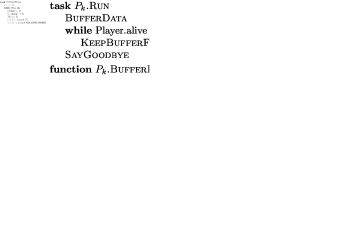
\includegraphics[width=0.75\textwidth]{chunk_generation_and_flooding}
  \fig{500}{5cm}{DBS_splitter_feed} \caption{Chunk
    generation at the splitter and their transmission to the
    team.\label{fig:chunk_generation}}
\end{figure*}
\end{comment}

A \gls{round} is defined as the process of transmitting $N$ different
chunks from the splitter to a team of $N\leq N^*$ peers (therefore,
all the peers of the team are origin of a different chunk, in each
round). For a team of size $N$, the average \gls{round-time} can be
estimated as
\begin{equation}
  t^{\mathrm{round}}=Nt^{\mathrm{chunk}},
\end{equation}
where $t^{\mathrm{chunk}}$ is the \gls{chunk-time}, defined as
\begin{equation}
  \label{eq:chunk_time}
  t^{\mathrm{chunk}}=\frac{l^{\mathrm{chunk}}}{R},
\end{equation}
where $l^{\mathrm{chunk}}$ is the length of the chunks (all the chunks are
split with the same length) and $R$ is the average transmission
bit-rate, that should match the average bit-rate of the stream in
order to achieve a seamsless playing.

\begin{comment}
The round-time is defined by:
\begin{equation}
  \cal{r} = \cal{c}N.
  \label{eq:round_time}
\end{equation}
For example, if we use only one team of $N=256$ peers, a chunk size
$C=1024$~bytes, and a video of $1$~Mb/s, the round time is
\begin{displaymath}
  \cal{r} = \frac{1024\frac{\text{bytes}}{\text{chunk}}\times
    8\frac{\text{bits}}{\text{byte}}}{10^6\frac{\text{bits}}{\text{second}}}\times
  256 \approx 2.1~\text{seconds}.
\end{displaymath}
\end{comment}


\subsection{Joining a team}
% Emacs, this is -*-latex-*-

% Joining the Team

\label{sec:joining}

After connecting with a splitter, incoming peers request (using a
reliable communication) to the splitter the current set of peers in
the team. To minimize the joining time, the peer sends a
$[\mathtt{hello}]$ message to each other peer of the team, in parallel
with the reception of the set. When a peer of the team receives a
$[\mathtt{hello}]$, it adds the sender of the message to a
\emph{table}\footnote{A structure which implements a random access
  efficiently.} of peers called $\mathtt{forward}[]$ \note{(see
  \href{https://github.com/P2PSP/simulator/blob/f0c73be1817e7d3b816cc61cd2c8e59b17f9a0e6/src/core/peer_dbs.py\#L491}{$\text{forward[]}$
    in \texttt{peer.py}})}. If a peer $P_i$ has an entry
$\mathtt{forward}[P_j]=P_k$, then each chunk received by $P_i$ and
originated at $P_j$ will be forwarded to $P_k$. When an incoming peer
$P_i$ has received the set of peers, its forwarding table has been
initialized to $\mathtt{forward}[P_i]=\{\text{team}\setminus
P_i\}$. Notice that, as long as the forwarding table contains this
information, all chunks received from the splitter will be forwarded
to the rest of the team, directly (in one protocol hop). So, in
absence of communication constraints, the team will be organized as a
full-connected overlay (see Fig.~\ref{fig:full_mesh}).

%), initializes
%the table $\mathrm{debt}[]$ (which stores the chunk debts between
%neighbor peers), and (3) sets the variable $\mathrm{neighbor}$ with an
%index to $\mathrm{forward}[]$ (see
%Sec.~\ref{sec:chunk_DBS_processing}).

The splitter, in an infinite loop: (1) listens to the incoming peers,
(2) sends to them the set of peers of the team, and (3) includes the
incoming peer to the set. Notice that only those peers that are in
the set of peers of the splitter are considered to be in the team
served by such splitter.

\begin{comment}
\begin{figure*}
  %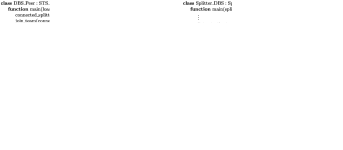
\includegraphics[width=\textwidth]{joining}
  \fig{1000}{10cm}{joining} \caption{Code related to team
    joining.\label{fig:joining}}
\end{figure*}

The new pseudo-code related to joining a team is describen in the
Fig.~\ref{fig:joining}.
\end{comment}

\begin{notex}
  See \href{https://github.com/P2PSP/simulator/blob/f0c73be1817e7d3b816cc61cd2c8e59b17f9a0e6/src/core/splitter_dbs.py#L296}{$\text{destination\_of\_chunk}[]$ in \texttt{peer\_dbs.py}}.
\end{notex}


\subsection{Buffering chunks}
%%% Local Variables:
%%% mode: latex
%%% TeX-master: "<none>"
%%% End:

\label{sec:buffering_chunks}

In order to hide the jitter generated by the physical network and the
protocol itself, peers need to store the received chunks in a buffer
during a period of time before playing them. A chunk with number $x$
is inserted in the position $(x \mathit{mod} 2B)$ of the buffer, where
$B$ is the maximum number of chunks that the buffer will store. In a
peer's life, $B$ is constant, but it is not compulsory that all peers
of the same team use the same $B$ value.

The buffer is implemented as a circular queue of $2B$ chunks, which is
filled up to only $B$ chunks in the buffering time (which is the main
part of the start-up time that the users experiment). Chunks with a
higher number (newer chunks) are inserted in the head of the
buffer. The chunk pointed by the tail of the buffer is sent to the
player (if there is a chunk in that cell of the buffer). This action
is carried out each time a new chunk is received.

Chunks can be lost.\footnote{Chunks are transmitted using a
  unrealiable communication, and therefore, network congestion can
  lose chunks.} A chunk is considered as lost when it is time to send
it to the player and the chunk has not been received.  In this
situation, for each lost chunk, the peer sends a $[\mathtt{request}
  \text{lost\_chunk\_number}]$ (that is the number of the next chunk
to be played) to the last neighbor served. When a peer $P_x$ receives
a $[\mathtt{request} \text{lost\_chunk\_number}]$ from $P_y$, $P_x$
adds $P_y$ to $\text{forward}[P_o]$, where $P_o$ is the origin peer of
the chunk stored in the position $lost\_chunk\_number$ of the buffer.

% As an alternative ...
\begin{comment}
origin peer of the next chunk stored in the
buffer. This peer has to characteristics: (1) it is not necessary a
neighbor peer, and (2) there is a high probability that this chunk has
been stored in the buffer ``for a long time'', so, if it is not a
neighbor, the link between it and the peer is working fairly well.
\end{comment}

\begin{notex}
  In the current implementation, the destination of the
  $[\mathtt{request} ...]$ message is the neighbor with the smaller
  chunk debt. This, a priori, has the drawback that this peer will
  always selected for relaying all the lost chunks because i will have
  a smaller debt as a consequence of the requests.
\end{notex}
  
In this situation, it is also possible that some peers can request
redundant paths between an origin peer and itself, and therefore, some
chunks could be received more than once. If this case, for each
duplicate chunk, a peer $P_i$ should send a $[\mathtt{prune}
  \text{duplicate\_chunk\_number}]$ message to those neighbors that
have sent to it the duplicate chunk. Neighbors receiving such message
from peer $P_i$ should remove the $P_i$ from $\text{forward}[P_o]$,
where $P_o$ is the origin peer of the duplicate chunk.

\begin{comment}
\begin{figure*}
  \fig{500}{5cm}{DBS_peer_buffering} \caption{Buffering of the
    chunks.\label{fig:DBS_peer_buffering}}
\end{figure*}
\end{comment}

The buffering time determines how much time the peers must wait before
start playing the chunks. Considering that chunks can be lost in
transit or delayed more than $B$ times of chunk, randomly, it is
difficult to determine, a priori the optimal buffering time. In the
current implementation, peers buffer a variable number of chunks that
depends on the order in which chunks are received. If $x_1$ is the
(number of the) first chunk received (the first chunk to be played),
the buffering time finishes when the chunk $x_1+B$ is
received.\footnote{Notice that all chunks with a number smaller than
  $x_1$ will be discarded, and that during the buffering time, it can
  happens that some chunks are not received on time. Therefore, it
  does not make sense to wait for $B$ chunks before stopping the
  buffering process.}

% Hablar de la relación entre B y el tamaño del team. Tal vez, cuando
% se presente la expresión de la latencia en función del grado de
% conectividad. En el caso extremo en que todos los peers se
% conectaran con todos, B >= N^*, el número máximo de peer en el team.

\begin{comment}
An heuristic that
works is the described in the Fig.~\ref{fig:DBS_peer_buffering}. As
can be seen, $\text{chunk\_to\_play}$ points to the first received
chunk, that not necessary is the received chunk with lower
index. After that, the
buffering finishes when a chunk with index $\text{chunk\_to\_play} +
\text{BUFFER\_SIZE}/2$ has been received.\footnote{This not means that
  $\text{BUFFER\_SIZE}/2$ chunks are available in the buffer.}
\end{comment}


\subsection{Chunk flooding}
\label{sec:chunk_flooding}
\begin{figure*}
  %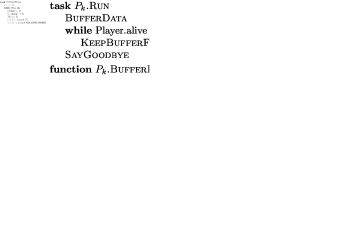
\includegraphics[width=0.75\textwidth]{chunk_generation_and_flooding}
  \fig{100}{3cm}{peer_chunk_flooding}
  \caption{Chunk flooding at peers.\label{fig:peer_chunk_flooding}}
\end{figure*}
When a peer $P_k$ receives a chunk from $P_i$, $P_k$ floods the
chunk to $T^k \setminus P_i$, using a prioritized round-robin
schema (see Fig.~\ref{fig:chunk_flooding}). Besides, if
it is a duplicate chunk, $P_k$ sends to $P_i$ a
$[\mathtt{NRFCF}~P_l]$ ($\mathtt{N}$ot $\mathtt{R}$elay
$\mathtt{F}$uture $\mathtt{C}$hunks $\mathtt{F}$rom) message, where
$P_l$ is the origin peer of the duplicate chunk. Thus, only
the first neighbor $P_i$ to send to $P_k$ a chunk
``originated'' at $P_l$ will do that in the future, at least
that $P_k$ revokes this routing information by sending a
$[\mathtt{RFCF}~P_l]$ ($\mathtt{R}$elay $\mathtt{F}$uture
$\mathtt{C}$hunks $\mathtt{F}$rom) to one or more (possibly the rest
of) peers of $T^k$.

As it has been said before, peers prioritize the flooding of the
chunks they relay by sending first the chunks to those neighbors that
are more supportive. To achieve that, every time $Pj_k$ sends a chunk
to $P_l$, $P_k$ runs $\mathtt{debt}[P_l] = \mathtt{debt}[P_l]+1$, and
$P_l$ runs $\mathtt{debt}[P_k] = \mathtt{debt}[P_k]-1$ (see
Fig.\ref{fig:}). Basically, these tables maintain a ``debt'' of chunks
between evey pair of neighbor peers. In ideal circunstances, debs
should be $0$. Debs are clipped to
$\pm\mathtt{debt}_{\text{max}}$. Obviously, a high supportivity means
a low debt, and viceversa.

\begin{comment}
In each round, peers check if a chunk have been received from the rest
of peers of the team (${\cal P}_k\in {\cal T}_j)$). If not, peers send
a $[\mathtt{propagate}~{\cal P}_i]$ to one or more (possibly
to the rest of) peers of the team, where ${\cal P}_i$ is the origin peer
of the missing chunk. At this point, the process continues as
described in Section~\ref{dbs:chunk_flooding}.
\end{comment}

\begin{comment}
For each ${\cal P}_k\in N({\cal P}_i)$, ${\cal P}_i$ checks if a chunk
has been received from ${\cal P}_k$. If ${\cal P}_i$ detects that
${\cal P}_k$ has not sent a chunk to it during $L$ consecutive rounds,
performs $N({\cal P}_i) = N({\cal P}_i)\setminus{\cal P}_k$, and stops
sending to ${\cal P}_k$ more chunks.
\end{comment}
\begin{comment}
computes a
``chunk-debt'', denoted by $d({\cal P}_k)$, that is incremented each
time a chunk is received from ${\cal P}_k$ and decremented each time a
chunk is sent to ${\cal P}_k$. If ${\cal P}_i$ verifies that $d({\cal
  P}_k)>D$ (the maximum debt), then ${\cal P}_i$ considers that ${\cal
  P}_k$ is unable to communicate with it, performs $N({\cal P}_i) =
N({\cal P}_i)\setminus{\cal P}_k$, and stops sending to ${\cal P}_k$
more chunks.
\end{comment}


%When peers receive chunks from their splitter, they must flood them to
%their neighbors until the chunks are broadcasted to the whole team
%(Fig.~\ref{fig:chunk_generation_and_flooding}). Lets suppose that
%${\cal P}_k$ receives a chunk. In the case the sender is its splitter,
%${\cal P}_k$ floods the chunk to $N({\cal P}_k)$. However, if the
%sender is a peer ${\cal P}_m\in N({\cal P}_k)$, ${\cal P}_k$ adds
%${\cal P}_m$ to $N({\cal P}_k)$ if ${\cal P}_m$ is a new neighbor, and
%forwards the chunk to the rest of its neighborhood ${\cal P}_n\in
%N({\cal P}_k)\setminus{\cal P}_m$ if ${\cal P}_k$ is in the shortest
%between ${\cal P}_n$ and the origin peer ${\cal P}_i$ of the relayed
%chunk. This will be true if ${\cal P}_k$ is the gateway of ${\cal
%  P}_n$ to go from ${\cal P}_n$ to ${\cal P}_i$. Therefore, a flooding
%with prunning based on shortest path routing is used.


\subsection{Routes discovery and topology optimization}
% Emacs, this is -*-latex-*-

% Routes Discovery and Topology Optimization

\label{sec:routes_discovery}

Chunks can be lost under bandwidth and buffering time constraints. A
chunk is lost when it is time to send it to the player, i.e. when it
is pointed by $p_p$, and the chunk has not been received. 
When a peer realizes that a chunk pointed by $p_p$ has been lost,
nothing can be done to recover it. Peers pre-fetch ``potentially
lost'' chunks at the buffer position $p_p+p_h$, where $p_h\geq 0$ is
the pre-feching horizon. Setting $p_h=0$, the pre-fetching is
disabled and only those chunks that really are lost will be
requested \leorem{no entiendo para que se piden}. 
On the contrary, the higher the $p_h$, the more aggressive
the pre-fetching is.  

For each (potentially) lost chunk with number
$\text{lost\_chunk\_number}$, peers send a
$[\mathtt{request}~\text{lost\_chunk\_number}]$ message to a random
peer of the team\leorem{solo uno? cuando se produce pruning?}. When a peer $P_i$ receives such message from 
$P_j$, $P_i$ adds $P_j$ to $\mathtt{forward}[P_k]$. $P_k$ is the
origin peer of the chunk stored in the position
$(\text{lost\_chunk\_number}~\mathit{mod}~2B)$ of $P_i$'s buffer in case this
chunks has been received. Otherwise, the request is ignored \leorem{y cómo se recupera?}. Notice
that, although request messages are very short, they are an overhead.

When request messages are used, redundant routes can be created and
therefore, some chunks could be received more than once. This is an overhead to be minimized. \leo{Upon the reception of the lost chunk, a peer send a pruning message to the other requested peers}. The receiver of the pruning message counts the number of times that a origin peer has been pruned, and when this counter is higher than a threshold $T$ (the maximum number of generated duplicates \leo{at requester's side}), the corresponding entry in the $\text{forward}[]$ table is deleted \leorem{Es por chunk o por origen?}.

Now, we can define more accurately the \gls{neighborhood-degree} (see
Sec.~\ref{sec:chunk_flooding}) as the number of different destination
peers for each possible origin that a peer forwards. For example, if a
peer $P_i$ forwards chunks from the origin $P_i$ to 10 neighbors, the
neighborhood degree of $P_i$ for the origin $P_i$ is 10, and if the
peer $P_i$ also forwards chunks from an origin $P_j$ to 5 neighbors,
the neighborhood degree of $P_i$ for the origin $P_j$ is 5\leorem{yo definiría dos tipos de grado de vecindad, el mio y el de reenvio}.

Considering the rules described before, the neighborhood degrees of
peers can decrease or increase to optimize the topology of the
overlay, by minimizing $\Delta t_b$. An increment in the degree for the origin of a requested
chunk $\text{lost\_chunk\_number}$ in $P_i$ is produced when $P_i$
recives a $[\mathtt{request}~\text{lost\_chunk\_number}]$ from a peer
that is not a neighbor, yet. On the contrary, a decrement in the
degree for the origin of a pruned chunk
$\text{duplicate\_chunk\_index}$ in $P_i$ is produced when $P_i$
receives a $[\mathtt{prune}~\text{duplicate\_chunk\_index}]$ from a
neighbor peer, for that origin. In fact, the continued use of the
requesting and pruning messages produce in a peer $P_i$ that the list
$\text{forward}[P_i]$ gets shorter (smaller \gls{neighborhood-degree})
and new entries in the table $\text{forward}[]$ are created.


%\subsection{Overlay topology optimization and the neighborhood degree}
%The neighborhood degree can also grow. When a chunk is lost, the peer
requests to receive the rest of chunks from the corresponding origin
peer to a random peer of the team. If duplicates are generated, prune
messages will remove the slower routes from that origin peer,
generating that the most reliable (and possiblely faster) route to
endure. When this happens, the requesting peer will be added to
$\mathtt{forward}[]$ (and therefore, sooner or later to
$\mathtt{pending}[]$) table of the requested peer, increasing its
neighborhood degree.


\subsection{Leaving a team}
\begin{figure*}
  %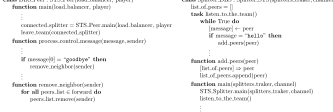
\includegraphics[width=0.55\textwidth]{leaving}
  \fig{300}{4cm}{leaving}
  \caption{Peer leaving.\label{fig:leaving}}
\end{figure*}
An outgoing peer $P^t_o$ (see Fig.~\ref{fig:leaving}) must to: (1) say
$[\mathtt{goodbye}]$ to $S^t$ and to $T^t_o$ (in this order), (2)
relay any pending (received but yet not sent) chunks, and (3) wait for
a $[\mathtt{goodbye}]$ from $S^t$, which performs $T^t = T^t \setminus
P^t_o$. In case of a timeout, $P^t_o$ resets the leaving procedure,
for a maximum number of times.

When a $P^t_k$ receives a $[\mathtt{goodbye}]$ from $P^t_o$, $P^t_k$
removes $P^t_o$ from its neighbors set, by running $T^t_k = T^t_k
\setminus P^t_o$.


\subsection{Free-riding control}
% Emacs, this is -*-latex-*-

% Free-riding Control at the Splitter

\label{sec:free_riding_control}

The splitter remembers which chunk, of a list of the last $B'$
transmitted chunks, was sent to each peer of the team. Notice that, in
order to remember the chunk that was sent to each peer in each round,
it must be hold that $B'\ge N$. \note{See
  \href{https://github.com/P2PSP/simulator/blob/f0c73be1817e7d3b816cc61cd2c8e59b17f9a0e6/src/core/splitter_dbs.py\#L296}{$\text{destination\_of\_chunk}[]$
    in \texttt{splitter\_dbs.py}}.}

Monitor peers (which are trusted peers) complain to their splitter
with a $[\mathtt{lost}~\text{lost\_chunk\_number}]$ for each lost
chunk. The splitter only considers these type of messages if they come
from a monitor.

%Notice that $L$ will
%tend to be proportional to the number $M$ of monitors, especially if
%those cases where $P_o$ is a gone peer that was unable to transmit the
%$[\mathtt{goodbye}]$ messages.

\begin{notex}
This last functionality has not been implemented, at least, as it has
been explained here. The forget() thread is controlled by a timer, not
by a counter of rounds.
\end{notex}

%Peers also control that at least one chunk is received from a neighbor
%in each round.\footnote{Peers recognize that a new round has started
%  when a new chunk is received from the splitter.} If happens that a
%peer $P_x$ does not receives a chunk from peer $P_y$ between $D^*$
%consecutive rounds, $P_x$ removes $P_y$ of its forwaring table.


%\subsection{Free-riding control at peers} % Neighborhood dynamics
%\label{dbs:frcp}
%Every time ${\cal P}^j_k$ sends a chunk to ${\cal P}^j_l$, ${\cal
P}^j_k$ runs $\mathtt{debt}[{\cal P}^j_l] = \mathtt{debt}[{\cal
P}^j_l]+1$, and ${\cal P}^j_l$ runs $\mathtt{debt}[{\cal P}^j_k]
= \mathtt{debt}[{\cal P}^j_k]-1$ (see Fig.\ref{fig}). Basically, these tables
maintain a ``debt'' of chunks between evey pair of neighbor
peers. If ${\cal P}^j_k$ realises that $\mathtt{debt}[{\cal
P}^j_l]>\mathtt{debt}_\text{max}$, then ${\cal P}^j_k$ removes ${\cal
P}^j_l$ from ${\cal T}^j_k$. Debts are clipped to $0$.

\begin{comment}
In each round, peers check if a chunk have been received from the rest
of peers of the team (${\cal P}_k\in {\cal T}_j)$). If not, peers send
a $[\mathtt{propagate}~{\cal P}_i]$ to one or more (possibly
to the rest of) peers of the team, where ${\cal P}_i$ is the origin peer
of the missing chunk. At this point, the process continues as
described in Section~\ref{dbs:chunk_flooding}.
\end{comment}

\begin{comment}
For each ${\cal P}_k\in N({\cal P}_i)$, ${\cal P}_i$ checks if a chunk
has been received from ${\cal P}_k$. If ${\cal P}_i$ detects that
${\cal P}_k$ has not sent a chunk to it during $L$ consecutive rounds,
performs $N({\cal P}_i) = N({\cal P}_i)\setminus{\cal P}_k$, and stops
sending to ${\cal P}_k$ more chunks.
\end{comment}
\begin{comment}
computes a
``chunk-debt'', denoted by $d({\cal P}_k)$, that is incremented each
time a chunk is received from ${\cal P}_k$ and decremented each time a
chunk is sent to ${\cal P}_k$. If ${\cal P}_i$ verifies that $d({\cal
  P}_k)>D$ (the maximum debt), then ${\cal P}_i$ considers that ${\cal
  P}_k$ is unable to communicate with it, performs $N({\cal P}_i) =
N({\cal P}_i)\setminus{\cal P}_k$, and stops sending to ${\cal P}_k$
more chunks.
\end{comment}


%\subsection{Congestion control}
%\label{dbs:congestion_control}
%P2PSP is a content-unaware push-based protocol. To avoid network
congestion while flooding, sending peers must perform some kind of
data flow-control. Moreover, to achieve aN ideal I/O ratio of $1$,
peers should send one chunk for every received one.

Congestion control in P2PSP is very simple: if a new chunk is
received, peers forward (using the flooding with prunning algorithm
described in Sec~\ref{dbs:chunk_generation_and_flooding}) each
received chunk to the next peer of their list of peers (following a
round-robin pattern).

%Peers do not understand the content, but it is
%known that in order to achieve a I/O ratio of 1, peers should send one
%chunk for every received one, on average. To acomplish this, a ${\cal
%  P}_i$ creates a FIFO queue of chunks for each $N({\cal P}_i)$, and,
%for each received chunk, ${\cal P}_i$ forwards a queued chunk from
%each of these queues.

\begin{comment}
A ${\cal P}_i$ forwards one or more chunks if and only if it has
received a chunk. For each received chunk $c_j$, ${\cal P}_i$: 1)
creates a list $l_{c_j}$ with the contents of $N'({\cal P}_i)$, and 2)
sends $c_j$ to $l_{c_j}[0]$ (the first element), and removes
$l_{c_j}[0]$. For each chunk reception, Step 2) is repeated for all
the previously created lists while they are not exhausted.

A solution is a forwarding algorithm based on the following
idea. Peers manage a list of chunks, where every item is a 2-tuple
($c_k$, $P_l$). The field $c_k$ represents the chunk that must be
flooded (if the node that has delivered the chunk is the splitter,
$c_k$ must be relayed towards all the neighbors, otherwise, $c_k$ must
be sent to all the neighbors except the peer that delivered $c_k$),
and the field $P_l$ the last neighbor to which $c_k$ was sent. For
every chunk received, a new tuple is appended to the list of chunks
and the rest of tuples are updated. The field $c_k$ remains constant
but $P_l$ is replaced by the next peer in the list of neighbors for
every received chunk.
\end{comment}


\begin{comment}
\subsubsection{Flooding order}
\label{dbs:flooding_order}
As an incentive mechanism~\cite{xu2006analysis}, peers relay received
chunks first to those peers that 
\end{comment}

%neighbors with lower chunk-debts.

\begin{comment}
\subsubsection{Team dynamics}
\label{dbs:team_dynamics}
${\cal P}_i$ adds to $N({\cal P}_i)$ those ${\cal P}_j$ that has sent
to ${\cal P}_i$ a chunk. If $N({\cal P}_i)>K$, periodically, ${\cal
  P}_i$ removes from $N({\cal P}_i)$ the peer with highest chunk-debt
and try to find in ${\cal T}_j\setminus N({\cal P}_i)$ a new peer using
$[\mathtt{hello}]$ messages.
\end{comment}

\begin{comment}
Peers use a buffer $b$ of chunks to hide the jitter generated by the
physical network and the broadcasting protocol. When a peer receives
$C_i$, it performs
\begin{equation}
  b[i~\text{mod}~B] = c_i,
\end{equation}
where ``mod'' represents the modulo operator and $B$ the buffer size
(in chunks). Basically, the buffer represents a sliding window that
moves over the stream synchronizely with the playing because the the
player consumes the chunks at the same chunk-rate the source produces
them.
\end{comment}

%%%%%%%%%%

\begin{comment}

\begin{itemize}

\item In the P2PSP, only monitor peers complains about lost
  chunks. This means that if a chunk that has been retransmitted by a
  peer is lost, it will be only retransmitted to all the peers of the
  team if the destination is a monitor peer and there is a unique
  monitor peer in the team. On the other hand, if the lost chunk was
  traveling from the splitter to a peer, all monitor peers will
  complain and this chunk will be retransmitted to the complete
  team. Therefore, only massively loss chunks will be retransmitted in
  the P2PSP. However, notice that a isolated missing chunk will
  produce negligible artifacts in the playback of one peer. In the
  Chain model, the lost of a chunk is handled between neighbour peers
  which means that all lost blocks should be, a priori, recovered.

\end{itemize}

\end{comment}



\begin{comment}
\subsubsection{Shortest path computation}
\label{dbs:chunk_routing}
\begin{figure}
  %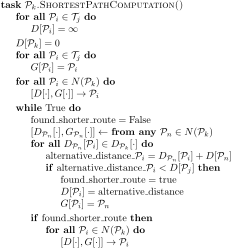
\includegraphics[width=0.35\textwidth]{shortest_path_computation}
  \fig{500}{4cm}{shortest_path_computation}
  \caption{Shortest path computation.\label{fig:shortest_path_computation}}
\end{figure}
The shortest path distances among peers are determined by a variation
of the Bellman-Ford Algorithm~\cite{Bertsekas1987data} (see
Fig.~\ref{fig:shortest_path_computation}), where the cost of the
``links'' between neighbor peers is $1$. Neighbor peers interchange
two vectors $D[\cdot]$ (distance-to-peer) and $G[\cdot]$
(gateway-to-peer) and compute the shortest distances and the (peer)
gateways to (reach) the rest of peers of its team ${\cal T}_j$.

This algorithm is free of routing loops and is not suceptible of the
well known count-to-infinity problem, and therefore always converges
for static teams. These problems do not appear because the routes are 

Each peer ${\cal P}_k$ sends
its vector of distances $D[\forall {\cal P}_i\in T^*({\cal P}_k)]$ and
gateways $G[\forall {\cal P}_i\in T^*({\cal P}_k)]$ to each
neighbor. When this information is received, peers check if shorter
routes can be found to the rest of peers of the reachable team, and if
so, send these vectors again.

The Bellman-Ford algorithm is susceptible of routing loops and the
count-to-infinite problem.


% Hace falta saber desde dónde viene el chunk original (origin peer) y que todos los peers dispongan de los vector-distances de los peers vecinos. Los vector-ditances deben tener tantas entradas como peers existen en el team. Por tanto, cada peer almacena un número de vector-distances igual a su grado de conectividad.


% Supposing that the weight of links between neighbors is 1.
% ¿Cómo sabe un peer que él es el último?
\end{comment}

\begin{comment}
\subsubsection{Generation of the routing tables}
Routing tables has as many entries as peers are in the team. The
routing table of a peer $P_i$ is a dictionary of pairs ($d(P_i, P_j)$,
$P_k$) indexed by the destination peer $P_j$ is a destination peer,
where $d(P_i, P_j)$ is the last measurement of the number of hops (in
peers) between $P_i$ and $P_j$, and $P_k\in N(P_i)$ is the 1-hop peer
that in the shortest-path between $P_i$ and $P_j$. Notice that if
$P_j==P_k$ then $d(P_i, P_j)==1$, which means that $P_i$ and $P_j$ are
directly ``connected''.

When a peer has updated its routing table, it is sent to their
neighbors pyggibacked on a \textsf{chunk} packet. When a peer receives
a routing table, it keeps a copy of it and updates its own routing
table with the new routing information using the Bellman-Ford
Algorithm~\cite{}. The peers have a copy of the routing table of its
neighbors to use it through the chunk routing process (see
Rule~\cite{the_routing_process}.
\end{comment}



\section{DBS (Data Broadcasting Set)}
\label{sec:DBS}
DBS provides ALM for unicast (TCP/UDP) environments. The media is
received by a collection of
\emph{splitters} ${\cal S}=\{{\cal S}^0, \cdots, {\cal
  S}^{G-1}\}$ from a streaming server ${\cal O}$,
called \emph{source}, at a (usually variable) bit-rate which matches
the bit-rate of the media. Each ${\cal S}^i$ splits the
stream into a sequence of \emph{chunks}, and relay them to
different \emph{team} of up to $N$ \emph{peers}. We define the set of
teams as ${\cal T}=\{{\cal T}^0,\cdots,{\cal T}^{G-1}\}$ and the set
of peers per team $T^j=\{{\cal P}^j_0,\cdots,{\cal P}^j_{N-1}\}$.


%${\cal T}=\{{\cal T}_0,\cdots,{\cal T}_{G-1}\}$ \emph{teams} (one per
%  splitter) of up to $N$
%\emph{peers} $\{{\cal P}_0,\cdots,{\cal P}_{N-1}\}$, per team.


\subsection{Team definition and types of peers}
%%% Local Variables:
%%% mode: latex
%%% TeX-master: "<none>"
%%% End:

\label{sec:team_def}

A team is a set of one or more peers that share the same stream. By
definition, in a team of size one (the corresponding splitter is
considered out of the team if feeds), the only peer is known as a
\emph{monitor} peer, and in a team with more than one peer, at least
one of them must be a monitor peer. Monitors are instantiated by the
team administrator to monitorize different aspects of the
broadcasting, such as, the expected quality of the rendered video at
the peers or the expected average end-user latency.


\subsection{Feeding the team}
% Emacs, this is -*-latex-*-

% Feeding the Team

\label{sec:feeding_the_team}

The splitter divides the stream into chunks of constant length $C$,
and sends exclusively each chunk to a different
\gls{origin}\footnote{In the route that a chunk traces from the
  splitter to all peers of the team, the origin peer is the first one
  in this route i.e., the peer selected by the splitter for that
  chunk.}  peer, using a round-robin schema. Chunks are enumerated to
distinguish them, and this information is transmitted as a part of a chunk
header.

\begin{comment}
More details about the implementation
are available in Fig.~\ref{fig:chunk_generation}.

%$x$, conforming a message
%$c_x=[x,\text{chunk}]$, where
%$x=i \text{mod} \text{Splitter\_DBS.list\_of\_peers}.\text{length}()$.

\begin{figure*}
  %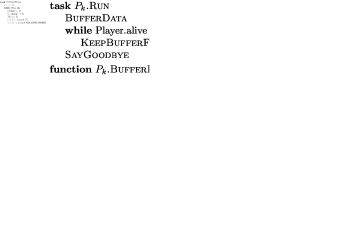
\includegraphics[width=0.75\textwidth]{chunk_generation_and_flooding}
  \fig{500}{5cm}{DBS_splitter_feed} \caption{Chunk
    generation at the splitter and their transmission to the
    team.\label{fig:chunk_generation}}
\end{figure*}
\end{comment}

A \gls{round} is defined as the process of transmitting $N$ different
chunks from the splitter to a team of $N\leq N^*$ peers (therefore,
all the peers of the team are origin of a different chunk, in each
round). For a team of size $N$, the average \gls{round-time} can be
estimated as
\begin{equation}
  t^{\mathrm{round}}=Nt^{\mathrm{chunk}},
\end{equation}
where $t^{\mathrm{chunk}}$ is the \gls{chunk-time}, defined as
\begin{equation}
  \label{eq:chunk_time}
  t^{\mathrm{chunk}}=\frac{l^{\mathrm{chunk}}}{R},
\end{equation}
where $l^{\mathrm{chunk}}$ is the length of the chunks (all the chunks are
split with the same length) and $R$ is the average transmission
bit-rate, that should match the average bit-rate of the stream in
order to achieve a seamsless playing.

\begin{comment}
The round-time is defined by:
\begin{equation}
  \cal{r} = \cal{c}N.
  \label{eq:round_time}
\end{equation}
For example, if we use only one team of $N=256$ peers, a chunk size
$C=1024$~bytes, and a video of $1$~Mb/s, the round time is
\begin{displaymath}
  \cal{r} = \frac{1024\frac{\text{bytes}}{\text{chunk}}\times
    8\frac{\text{bits}}{\text{byte}}}{10^6\frac{\text{bits}}{\text{second}}}\times
  256 \approx 2.1~\text{seconds}.
\end{displaymath}
\end{comment}


\subsection{Joining a team}
% Emacs, this is -*-latex-*-

% Joining the Team

\label{sec:joining}

After connecting with a splitter, incoming peers request (using a
reliable communication) to the splitter the current set of peers in
the team. To minimize the joining time, the peer sends a
$[\mathtt{hello}]$ message to each other peer of the team, in parallel
with the reception of the set. When a peer of the team receives a
$[\mathtt{hello}]$, it adds the sender of the message to a
\emph{table}\footnote{A structure which implements a random access
  efficiently.} of peers called $\mathtt{forward}[]$ \note{(see
  \href{https://github.com/P2PSP/simulator/blob/f0c73be1817e7d3b816cc61cd2c8e59b17f9a0e6/src/core/peer_dbs.py\#L491}{$\text{forward[]}$
    in \texttt{peer.py}})}. If a peer $P_i$ has an entry
$\mathtt{forward}[P_j]=P_k$, then each chunk received by $P_i$ and
originated at $P_j$ will be forwarded to $P_k$. When an incoming peer
$P_i$ has received the set of peers, its forwarding table has been
initialized to $\mathtt{forward}[P_i]=\{\text{team}\setminus
P_i\}$. Notice that, as long as the forwarding table contains this
information, all chunks received from the splitter will be forwarded
to the rest of the team, directly (in one protocol hop). So, in
absence of communication constraints, the team will be organized as a
full-connected overlay (see Fig.~\ref{fig:full_mesh}).

%), initializes
%the table $\mathrm{debt}[]$ (which stores the chunk debts between
%neighbor peers), and (3) sets the variable $\mathrm{neighbor}$ with an
%index to $\mathrm{forward}[]$ (see
%Sec.~\ref{sec:chunk_DBS_processing}).

The splitter, in an infinite loop: (1) listens to the incoming peers,
(2) sends to them the set of peers of the team, and (3) includes the
incoming peer to the set. Notice that only those peers that are in
the set of peers of the splitter are considered to be in the team
served by such splitter.

\begin{comment}
\begin{figure*}
  %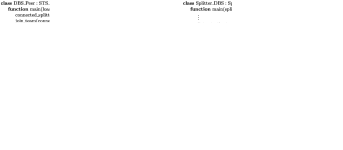
\includegraphics[width=\textwidth]{joining}
  \fig{1000}{10cm}{joining} \caption{Code related to team
    joining.\label{fig:joining}}
\end{figure*}

The new pseudo-code related to joining a team is describen in the
Fig.~\ref{fig:joining}.
\end{comment}

\begin{notex}
  See \href{https://github.com/P2PSP/simulator/blob/f0c73be1817e7d3b816cc61cd2c8e59b17f9a0e6/src/core/splitter_dbs.py#L296}{$\text{destination\_of\_chunk}[]$ in \texttt{peer\_dbs.py}}.
\end{notex}


\subsection{Buffering chunks}
%%% Local Variables:
%%% mode: latex
%%% TeX-master: "<none>"
%%% End:

\label{sec:buffering_chunks}

In order to hide the jitter generated by the physical network and the
protocol itself, peers need to store the received chunks in a buffer
during a period of time before playing them. A chunk with number $x$
is inserted in the position $(x \mathit{mod} 2B)$ of the buffer, where
$B$ is the maximum number of chunks that the buffer will store. In a
peer's life, $B$ is constant, but it is not compulsory that all peers
of the same team use the same $B$ value.

The buffer is implemented as a circular queue of $2B$ chunks, which is
filled up to only $B$ chunks in the buffering time (which is the main
part of the start-up time that the users experiment). Chunks with a
higher number (newer chunks) are inserted in the head of the
buffer. The chunk pointed by the tail of the buffer is sent to the
player (if there is a chunk in that cell of the buffer). This action
is carried out each time a new chunk is received.

Chunks can be lost.\footnote{Chunks are transmitted using a
  unrealiable communication, and therefore, network congestion can
  lose chunks.} A chunk is considered as lost when it is time to send
it to the player and the chunk has not been received.  In this
situation, for each lost chunk, the peer sends a $[\mathtt{request}
  \text{lost\_chunk\_number}]$ (that is the number of the next chunk
to be played) to the last neighbor served. When a peer $P_x$ receives
a $[\mathtt{request} \text{lost\_chunk\_number}]$ from $P_y$, $P_x$
adds $P_y$ to $\text{forward}[P_o]$, where $P_o$ is the origin peer of
the chunk stored in the position $lost\_chunk\_number$ of the buffer.

% As an alternative ...
\begin{comment}
origin peer of the next chunk stored in the
buffer. This peer has to characteristics: (1) it is not necessary a
neighbor peer, and (2) there is a high probability that this chunk has
been stored in the buffer ``for a long time'', so, if it is not a
neighbor, the link between it and the peer is working fairly well.
\end{comment}

\begin{notex}
  In the current implementation, the destination of the
  $[\mathtt{request} ...]$ message is the neighbor with the smaller
  chunk debt. This, a priori, has the drawback that this peer will
  always selected for relaying all the lost chunks because i will have
  a smaller debt as a consequence of the requests.
\end{notex}
  
In this situation, it is also possible that some peers can request
redundant paths between an origin peer and itself, and therefore, some
chunks could be received more than once. If this case, for each
duplicate chunk, a peer $P_i$ should send a $[\mathtt{prune}
  \text{duplicate\_chunk\_number}]$ message to those neighbors that
have sent to it the duplicate chunk. Neighbors receiving such message
from peer $P_i$ should remove the $P_i$ from $\text{forward}[P_o]$,
where $P_o$ is the origin peer of the duplicate chunk.

\begin{comment}
\begin{figure*}
  \fig{500}{5cm}{DBS_peer_buffering} \caption{Buffering of the
    chunks.\label{fig:DBS_peer_buffering}}
\end{figure*}
\end{comment}

The buffering time determines how much time the peers must wait before
start playing the chunks. Considering that chunks can be lost in
transit or delayed more than $B$ times of chunk, randomly, it is
difficult to determine, a priori the optimal buffering time. In the
current implementation, peers buffer a variable number of chunks that
depends on the order in which chunks are received. If $x_1$ is the
(number of the) first chunk received (the first chunk to be played),
the buffering time finishes when the chunk $x_1+B$ is
received.\footnote{Notice that all chunks with a number smaller than
  $x_1$ will be discarded, and that during the buffering time, it can
  happens that some chunks are not received on time. Therefore, it
  does not make sense to wait for $B$ chunks before stopping the
  buffering process.}

% Hablar de la relación entre B y el tamaño del team. Tal vez, cuando
% se presente la expresión de la latencia en función del grado de
% conectividad. En el caso extremo en que todos los peers se
% conectaran con todos, B >= N^*, el número máximo de peer en el team.

\begin{comment}
An heuristic that
works is the described in the Fig.~\ref{fig:DBS_peer_buffering}. As
can be seen, $\text{chunk\_to\_play}$ points to the first received
chunk, that not necessary is the received chunk with lower
index. After that, the
buffering finishes when a chunk with index $\text{chunk\_to\_play} +
\text{BUFFER\_SIZE}/2$ has been received.\footnote{This not means that
  $\text{BUFFER\_SIZE}/2$ chunks are available in the buffer.}
\end{comment}


\subsection{Chunk flooding}
\label{sec:chunk_flooding}
\begin{figure*}
  %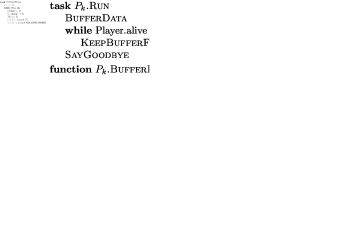
\includegraphics[width=0.75\textwidth]{chunk_generation_and_flooding}
  \fig{100}{3cm}{peer_chunk_flooding}
  \caption{Chunk flooding at peers.\label{fig:peer_chunk_flooding}}
\end{figure*}
When a peer $P_k$ receives a chunk from $P_i$, $P_k$ floods the
chunk to $T^k \setminus P_i$, using a prioritized round-robin
schema (see Fig.~\ref{fig:chunk_flooding}). Besides, if
it is a duplicate chunk, $P_k$ sends to $P_i$ a
$[\mathtt{NRFCF}~P_l]$ ($\mathtt{N}$ot $\mathtt{R}$elay
$\mathtt{F}$uture $\mathtt{C}$hunks $\mathtt{F}$rom) message, where
$P_l$ is the origin peer of the duplicate chunk. Thus, only
the first neighbor $P_i$ to send to $P_k$ a chunk
``originated'' at $P_l$ will do that in the future, at least
that $P_k$ revokes this routing information by sending a
$[\mathtt{RFCF}~P_l]$ ($\mathtt{R}$elay $\mathtt{F}$uture
$\mathtt{C}$hunks $\mathtt{F}$rom) to one or more (possibly the rest
of) peers of $T^k$.

As it has been said before, peers prioritize the flooding of the
chunks they relay by sending first the chunks to those neighbors that
are more supportive. To achieve that, every time $Pj_k$ sends a chunk
to $P_l$, $P_k$ runs $\mathtt{debt}[P_l] = \mathtt{debt}[P_l]+1$, and
$P_l$ runs $\mathtt{debt}[P_k] = \mathtt{debt}[P_k]-1$ (see
Fig.\ref{fig:}). Basically, these tables maintain a ``debt'' of chunks
between evey pair of neighbor peers. In ideal circunstances, debs
should be $0$. Debs are clipped to
$\pm\mathtt{debt}_{\text{max}}$. Obviously, a high supportivity means
a low debt, and viceversa.

\begin{comment}
In each round, peers check if a chunk have been received from the rest
of peers of the team (${\cal P}_k\in {\cal T}_j)$). If not, peers send
a $[\mathtt{propagate}~{\cal P}_i]$ to one or more (possibly
to the rest of) peers of the team, where ${\cal P}_i$ is the origin peer
of the missing chunk. At this point, the process continues as
described in Section~\ref{dbs:chunk_flooding}.
\end{comment}

\begin{comment}
For each ${\cal P}_k\in N({\cal P}_i)$, ${\cal P}_i$ checks if a chunk
has been received from ${\cal P}_k$. If ${\cal P}_i$ detects that
${\cal P}_k$ has not sent a chunk to it during $L$ consecutive rounds,
performs $N({\cal P}_i) = N({\cal P}_i)\setminus{\cal P}_k$, and stops
sending to ${\cal P}_k$ more chunks.
\end{comment}
\begin{comment}
computes a
``chunk-debt'', denoted by $d({\cal P}_k)$, that is incremented each
time a chunk is received from ${\cal P}_k$ and decremented each time a
chunk is sent to ${\cal P}_k$. If ${\cal P}_i$ verifies that $d({\cal
  P}_k)>D$ (the maximum debt), then ${\cal P}_i$ considers that ${\cal
  P}_k$ is unable to communicate with it, performs $N({\cal P}_i) =
N({\cal P}_i)\setminus{\cal P}_k$, and stops sending to ${\cal P}_k$
more chunks.
\end{comment}


%When peers receive chunks from their splitter, they must flood them to
%their neighbors until the chunks are broadcasted to the whole team
%(Fig.~\ref{fig:chunk_generation_and_flooding}). Lets suppose that
%${\cal P}_k$ receives a chunk. In the case the sender is its splitter,
%${\cal P}_k$ floods the chunk to $N({\cal P}_k)$. However, if the
%sender is a peer ${\cal P}_m\in N({\cal P}_k)$, ${\cal P}_k$ adds
%${\cal P}_m$ to $N({\cal P}_k)$ if ${\cal P}_m$ is a new neighbor, and
%forwards the chunk to the rest of its neighborhood ${\cal P}_n\in
%N({\cal P}_k)\setminus{\cal P}_m$ if ${\cal P}_k$ is in the shortest
%between ${\cal P}_n$ and the origin peer ${\cal P}_i$ of the relayed
%chunk. This will be true if ${\cal P}_k$ is the gateway of ${\cal
%  P}_n$ to go from ${\cal P}_n$ to ${\cal P}_i$. Therefore, a flooding
%with prunning based on shortest path routing is used.


\subsection{Routes discovery and topology optimization}
% Emacs, this is -*-latex-*-

% Routes Discovery and Topology Optimization

\label{sec:routes_discovery}

Chunks can be lost under bandwidth and buffering time constraints. A
chunk is lost when it is time to send it to the player, i.e. when it
is pointed by $p_p$, and the chunk has not been received. 
When a peer realizes that a chunk pointed by $p_p$ has been lost,
nothing can be done to recover it. Peers pre-fetch ``potentially
lost'' chunks at the buffer position $p_p+p_h$, where $p_h\geq 0$ is
the pre-feching horizon. Setting $p_h=0$, the pre-fetching is
disabled and only those chunks that really are lost will be
requested \leorem{no entiendo para que se piden}. 
On the contrary, the higher the $p_h$, the more aggressive
the pre-fetching is.  

For each (potentially) lost chunk with number
$\text{lost\_chunk\_number}$, peers send a
$[\mathtt{request}~\text{lost\_chunk\_number}]$ message to a random
peer of the team\leorem{solo uno? cuando se produce pruning?}. When a peer $P_i$ receives such message from 
$P_j$, $P_i$ adds $P_j$ to $\mathtt{forward}[P_k]$. $P_k$ is the
origin peer of the chunk stored in the position
$(\text{lost\_chunk\_number}~\mathit{mod}~2B)$ of $P_i$'s buffer in case this
chunks has been received. Otherwise, the request is ignored \leorem{y cómo se recupera?}. Notice
that, although request messages are very short, they are an overhead.

When request messages are used, redundant routes can be created and
therefore, some chunks could be received more than once. This is an overhead to be minimized. \leo{Upon the reception of the lost chunk, a peer send a pruning message to the other requested peers}. The receiver of the pruning message counts the number of times that a origin peer has been pruned, and when this counter is higher than a threshold $T$ (the maximum number of generated duplicates \leo{at requester's side}), the corresponding entry in the $\text{forward}[]$ table is deleted \leorem{Es por chunk o por origen?}.

Now, we can define more accurately the \gls{neighborhood-degree} (see
Sec.~\ref{sec:chunk_flooding}) as the number of different destination
peers for each possible origin that a peer forwards. For example, if a
peer $P_i$ forwards chunks from the origin $P_i$ to 10 neighbors, the
neighborhood degree of $P_i$ for the origin $P_i$ is 10, and if the
peer $P_i$ also forwards chunks from an origin $P_j$ to 5 neighbors,
the neighborhood degree of $P_i$ for the origin $P_j$ is 5\leorem{yo definiría dos tipos de grado de vecindad, el mio y el de reenvio}.

Considering the rules described before, the neighborhood degrees of
peers can decrease or increase to optimize the topology of the
overlay, by minimizing $\Delta t_b$. An increment in the degree for the origin of a requested
chunk $\text{lost\_chunk\_number}$ in $P_i$ is produced when $P_i$
recives a $[\mathtt{request}~\text{lost\_chunk\_number}]$ from a peer
that is not a neighbor, yet. On the contrary, a decrement in the
degree for the origin of a pruned chunk
$\text{duplicate\_chunk\_index}$ in $P_i$ is produced when $P_i$
receives a $[\mathtt{prune}~\text{duplicate\_chunk\_index}]$ from a
neighbor peer, for that origin. In fact, the continued use of the
requesting and pruning messages produce in a peer $P_i$ that the list
$\text{forward}[P_i]$ gets shorter (smaller \gls{neighborhood-degree})
and new entries in the table $\text{forward}[]$ are created.


%\subsection{Overlay topology optimization and the neighborhood degree}
%The neighborhood degree can also grow. When a chunk is lost, the peer
requests to receive the rest of chunks from the corresponding origin
peer to a random peer of the team. If duplicates are generated, prune
messages will remove the slower routes from that origin peer,
generating that the most reliable (and possiblely faster) route to
endure. When this happens, the requesting peer will be added to
$\mathtt{forward}[]$ (and therefore, sooner or later to
$\mathtt{pending}[]$) table of the requested peer, increasing its
neighborhood degree.


\subsection{Leaving a team}
\begin{figure*}
  %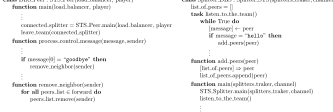
\includegraphics[width=0.55\textwidth]{leaving}
  \fig{300}{4cm}{leaving}
  \caption{Peer leaving.\label{fig:leaving}}
\end{figure*}
An outgoing peer $P^t_o$ (see Fig.~\ref{fig:leaving}) must to: (1) say
$[\mathtt{goodbye}]$ to $S^t$ and to $T^t_o$ (in this order), (2)
relay any pending (received but yet not sent) chunks, and (3) wait for
a $[\mathtt{goodbye}]$ from $S^t$, which performs $T^t = T^t \setminus
P^t_o$. In case of a timeout, $P^t_o$ resets the leaving procedure,
for a maximum number of times.

When a $P^t_k$ receives a $[\mathtt{goodbye}]$ from $P^t_o$, $P^t_k$
removes $P^t_o$ from its neighbors set, by running $T^t_k = T^t_k
\setminus P^t_o$.


\subsection{Free-riding control}
% Emacs, this is -*-latex-*-

% Free-riding Control at the Splitter

\label{sec:free_riding_control}

The splitter remembers which chunk, of a list of the last $B'$
transmitted chunks, was sent to each peer of the team. Notice that, in
order to remember the chunk that was sent to each peer in each round,
it must be hold that $B'\ge N$. \note{See
  \href{https://github.com/P2PSP/simulator/blob/f0c73be1817e7d3b816cc61cd2c8e59b17f9a0e6/src/core/splitter_dbs.py\#L296}{$\text{destination\_of\_chunk}[]$
    in \texttt{splitter\_dbs.py}}.}

Monitor peers (which are trusted peers) complain to their splitter
with a $[\mathtt{lost}~\text{lost\_chunk\_number}]$ for each lost
chunk. The splitter only considers these type of messages if they come
from a monitor.

%Notice that $L$ will
%tend to be proportional to the number $M$ of monitors, especially if
%those cases where $P_o$ is a gone peer that was unable to transmit the
%$[\mathtt{goodbye}]$ messages.

\begin{notex}
This last functionality has not been implemented, at least, as it has
been explained here. The forget() thread is controlled by a timer, not
by a counter of rounds.
\end{notex}

%Peers also control that at least one chunk is received from a neighbor
%in each round.\footnote{Peers recognize that a new round has started
%  when a new chunk is received from the splitter.} If happens that a
%peer $P_x$ does not receives a chunk from peer $P_y$ between $D^*$
%consecutive rounds, $P_x$ removes $P_y$ of its forwaring table.


%\subsection{Free-riding control at peers} % Neighborhood dynamics
%\label{dbs:frcp}
%Every time ${\cal P}^j_k$ sends a chunk to ${\cal P}^j_l$, ${\cal
P}^j_k$ runs $\mathtt{debt}[{\cal P}^j_l] = \mathtt{debt}[{\cal
P}^j_l]+1$, and ${\cal P}^j_l$ runs $\mathtt{debt}[{\cal P}^j_k]
= \mathtt{debt}[{\cal P}^j_k]-1$ (see Fig.\ref{fig}). Basically, these tables
maintain a ``debt'' of chunks between evey pair of neighbor
peers. If ${\cal P}^j_k$ realises that $\mathtt{debt}[{\cal
P}^j_l]>\mathtt{debt}_\text{max}$, then ${\cal P}^j_k$ removes ${\cal
P}^j_l$ from ${\cal T}^j_k$. Debts are clipped to $0$.

\begin{comment}
In each round, peers check if a chunk have been received from the rest
of peers of the team (${\cal P}_k\in {\cal T}_j)$). If not, peers send
a $[\mathtt{propagate}~{\cal P}_i]$ to one or more (possibly
to the rest of) peers of the team, where ${\cal P}_i$ is the origin peer
of the missing chunk. At this point, the process continues as
described in Section~\ref{dbs:chunk_flooding}.
\end{comment}

\begin{comment}
For each ${\cal P}_k\in N({\cal P}_i)$, ${\cal P}_i$ checks if a chunk
has been received from ${\cal P}_k$. If ${\cal P}_i$ detects that
${\cal P}_k$ has not sent a chunk to it during $L$ consecutive rounds,
performs $N({\cal P}_i) = N({\cal P}_i)\setminus{\cal P}_k$, and stops
sending to ${\cal P}_k$ more chunks.
\end{comment}
\begin{comment}
computes a
``chunk-debt'', denoted by $d({\cal P}_k)$, that is incremented each
time a chunk is received from ${\cal P}_k$ and decremented each time a
chunk is sent to ${\cal P}_k$. If ${\cal P}_i$ verifies that $d({\cal
  P}_k)>D$ (the maximum debt), then ${\cal P}_i$ considers that ${\cal
  P}_k$ is unable to communicate with it, performs $N({\cal P}_i) =
N({\cal P}_i)\setminus{\cal P}_k$, and stops sending to ${\cal P}_k$
more chunks.
\end{comment}


%\subsection{Congestion control}
%\label{dbs:congestion_control}
%P2PSP is a content-unaware push-based protocol. To avoid network
congestion while flooding, sending peers must perform some kind of
data flow-control. Moreover, to achieve aN ideal I/O ratio of $1$,
peers should send one chunk for every received one.

Congestion control in P2PSP is very simple: if a new chunk is
received, peers forward (using the flooding with prunning algorithm
described in Sec~\ref{dbs:chunk_generation_and_flooding}) each
received chunk to the next peer of their list of peers (following a
round-robin pattern).

%Peers do not understand the content, but it is
%known that in order to achieve a I/O ratio of 1, peers should send one
%chunk for every received one, on average. To acomplish this, a ${\cal
%  P}_i$ creates a FIFO queue of chunks for each $N({\cal P}_i)$, and,
%for each received chunk, ${\cal P}_i$ forwards a queued chunk from
%each of these queues.

\begin{comment}
A ${\cal P}_i$ forwards one or more chunks if and only if it has
received a chunk. For each received chunk $c_j$, ${\cal P}_i$: 1)
creates a list $l_{c_j}$ with the contents of $N'({\cal P}_i)$, and 2)
sends $c_j$ to $l_{c_j}[0]$ (the first element), and removes
$l_{c_j}[0]$. For each chunk reception, Step 2) is repeated for all
the previously created lists while they are not exhausted.

A solution is a forwarding algorithm based on the following
idea. Peers manage a list of chunks, where every item is a 2-tuple
($c_k$, $P_l$). The field $c_k$ represents the chunk that must be
flooded (if the node that has delivered the chunk is the splitter,
$c_k$ must be relayed towards all the neighbors, otherwise, $c_k$ must
be sent to all the neighbors except the peer that delivered $c_k$),
and the field $P_l$ the last neighbor to which $c_k$ was sent. For
every chunk received, a new tuple is appended to the list of chunks
and the rest of tuples are updated. The field $c_k$ remains constant
but $P_l$ is replaced by the next peer in the list of neighbors for
every received chunk.
\end{comment}


\begin{comment}
\subsubsection{Flooding order}
\label{dbs:flooding_order}
As an incentive mechanism~\cite{xu2006analysis}, peers relay received
chunks first to those peers that 
\end{comment}

%neighbors with lower chunk-debts.

\begin{comment}
\subsubsection{Team dynamics}
\label{dbs:team_dynamics}
${\cal P}_i$ adds to $N({\cal P}_i)$ those ${\cal P}_j$ that has sent
to ${\cal P}_i$ a chunk. If $N({\cal P}_i)>K$, periodically, ${\cal
  P}_i$ removes from $N({\cal P}_i)$ the peer with highest chunk-debt
and try to find in ${\cal T}_j\setminus N({\cal P}_i)$ a new peer using
$[\mathtt{hello}]$ messages.
\end{comment}

\begin{comment}
Peers use a buffer $b$ of chunks to hide the jitter generated by the
physical network and the broadcasting protocol. When a peer receives
$C_i$, it performs
\begin{equation}
  b[i~\text{mod}~B] = c_i,
\end{equation}
where ``mod'' represents the modulo operator and $B$ the buffer size
(in chunks). Basically, the buffer represents a sliding window that
moves over the stream synchronizely with the playing because the the
player consumes the chunks at the same chunk-rate the source produces
them.
\end{comment}

%%%%%%%%%%

\begin{comment}

\begin{itemize}

\item In the P2PSP, only monitor peers complains about lost
  chunks. This means that if a chunk that has been retransmitted by a
  peer is lost, it will be only retransmitted to all the peers of the
  team if the destination is a monitor peer and there is a unique
  monitor peer in the team. On the other hand, if the lost chunk was
  traveling from the splitter to a peer, all monitor peers will
  complain and this chunk will be retransmitted to the complete
  team. Therefore, only massively loss chunks will be retransmitted in
  the P2PSP. However, notice that a isolated missing chunk will
  produce negligible artifacts in the playback of one peer. In the
  Chain model, the lost of a chunk is handled between neighbour peers
  which means that all lost blocks should be, a priori, recovered.

\end{itemize}

\end{comment}



\begin{comment}
\subsubsection{Shortest path computation}
\label{dbs:chunk_routing}
\begin{figure}
  %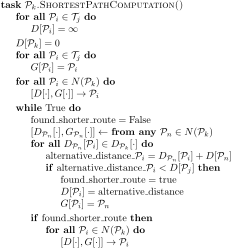
\includegraphics[width=0.35\textwidth]{shortest_path_computation}
  \fig{500}{4cm}{shortest_path_computation}
  \caption{Shortest path computation.\label{fig:shortest_path_computation}}
\end{figure}
The shortest path distances among peers are determined by a variation
of the Bellman-Ford Algorithm~\cite{Bertsekas1987data} (see
Fig.~\ref{fig:shortest_path_computation}), where the cost of the
``links'' between neighbor peers is $1$. Neighbor peers interchange
two vectors $D[\cdot]$ (distance-to-peer) and $G[\cdot]$
(gateway-to-peer) and compute the shortest distances and the (peer)
gateways to (reach) the rest of peers of its team ${\cal T}_j$.

This algorithm is free of routing loops and is not suceptible of the
well known count-to-infinity problem, and therefore always converges
for static teams. These problems do not appear because the routes are 

Each peer ${\cal P}_k$ sends
its vector of distances $D[\forall {\cal P}_i\in T^*({\cal P}_k)]$ and
gateways $G[\forall {\cal P}_i\in T^*({\cal P}_k)]$ to each
neighbor. When this information is received, peers check if shorter
routes can be found to the rest of peers of the reachable team, and if
so, send these vectors again.

The Bellman-Ford algorithm is susceptible of routing loops and the
count-to-infinite problem.


% Hace falta saber desde dónde viene el chunk original (origin peer) y que todos los peers dispongan de los vector-distances de los peers vecinos. Los vector-ditances deben tener tantas entradas como peers existen en el team. Por tanto, cada peer almacena un número de vector-distances igual a su grado de conectividad.


% Supposing that the weight of links between neighbors is 1.
% ¿Cómo sabe un peer que él es el último?
\end{comment}

\begin{comment}
\subsubsection{Generation of the routing tables}
Routing tables has as many entries as peers are in the team. The
routing table of a peer $P_i$ is a dictionary of pairs ($d(P_i, P_j)$,
$P_k$) indexed by the destination peer $P_j$ is a destination peer,
where $d(P_i, P_j)$ is the last measurement of the number of hops (in
peers) between $P_i$ and $P_j$, and $P_k\in N(P_i)$ is the 1-hop peer
that in the shortest-path between $P_i$ and $P_j$. Notice that if
$P_j==P_k$ then $d(P_i, P_j)==1$, which means that $P_i$ and $P_j$ are
directly ``connected''.

When a peer has updated its routing table, it is sent to their
neighbors pyggibacked on a \textsf{chunk} packet. When a peer receives
a routing table, it keeps a copy of it and updates its own routing
table with the new routing information using the Bellman-Ford
Algorithm~\cite{}. The peers have a copy of the routing table of its
neighbors to use it through the chunk routing process (see
Rule~\cite{the_routing_process}.
\end{comment}



\section{FCS (Free-riding Control Set)}
\label{sec:DBS}
DBS provides ALM for unicast (TCP/UDP) environments. The media is
received by a collection of
\emph{splitters} ${\cal S}=\{{\cal S}^0, \cdots, {\cal
  S}^{G-1}\}$ from a streaming server ${\cal O}$,
called \emph{source}, at a (usually variable) bit-rate which matches
the bit-rate of the media. Each ${\cal S}^i$ splits the
stream into a sequence of \emph{chunks}, and relay them to
different \emph{team} of up to $N$ \emph{peers}. We define the set of
teams as ${\cal T}=\{{\cal T}^0,\cdots,{\cal T}^{G-1}\}$ and the set
of peers per team $T^j=\{{\cal P}^j_0,\cdots,{\cal P}^j_{N-1}\}$.


%${\cal T}=\{{\cal T}_0,\cdots,{\cal T}_{G-1}\}$ \emph{teams} (one per
%  splitter) of up to $N$
%\emph{peers} $\{{\cal P}_0,\cdots,{\cal P}_{N-1}\}$, per team.


\subsection{Team definition and types of peers}
%%% Local Variables:
%%% mode: latex
%%% TeX-master: "<none>"
%%% End:

\label{sec:team_def}

A team is a set of one or more peers that share the same stream. By
definition, in a team of size one (the corresponding splitter is
considered out of the team if feeds), the only peer is known as a
\emph{monitor} peer, and in a team with more than one peer, at least
one of them must be a monitor peer. Monitors are instantiated by the
team administrator to monitorize different aspects of the
broadcasting, such as, the expected quality of the rendered video at
the peers or the expected average end-user latency.


\subsection{Feeding the team}
% Emacs, this is -*-latex-*-

% Feeding the Team

\label{sec:feeding_the_team}

The splitter divides the stream into chunks of constant length $C$,
and sends exclusively each chunk to a different
\gls{origin}\footnote{In the route that a chunk traces from the
  splitter to all peers of the team, the origin peer is the first one
  in this route i.e., the peer selected by the splitter for that
  chunk.}  peer, using a round-robin schema. Chunks are enumerated to
distinguish them, and this information is transmitted as a part of a chunk
header.

\begin{comment}
More details about the implementation
are available in Fig.~\ref{fig:chunk_generation}.

%$x$, conforming a message
%$c_x=[x,\text{chunk}]$, where
%$x=i \text{mod} \text{Splitter\_DBS.list\_of\_peers}.\text{length}()$.

\begin{figure*}
  %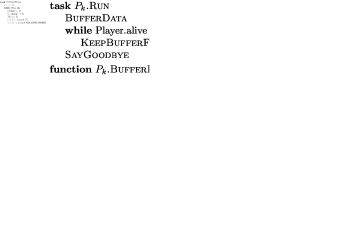
\includegraphics[width=0.75\textwidth]{chunk_generation_and_flooding}
  \fig{500}{5cm}{DBS_splitter_feed} \caption{Chunk
    generation at the splitter and their transmission to the
    team.\label{fig:chunk_generation}}
\end{figure*}
\end{comment}

A \gls{round} is defined as the process of transmitting $N$ different
chunks from the splitter to a team of $N\leq N^*$ peers (therefore,
all the peers of the team are origin of a different chunk, in each
round). For a team of size $N$, the average \gls{round-time} can be
estimated as
\begin{equation}
  t^{\mathrm{round}}=Nt^{\mathrm{chunk}},
\end{equation}
where $t^{\mathrm{chunk}}$ is the \gls{chunk-time}, defined as
\begin{equation}
  \label{eq:chunk_time}
  t^{\mathrm{chunk}}=\frac{l^{\mathrm{chunk}}}{R},
\end{equation}
where $l^{\mathrm{chunk}}$ is the length of the chunks (all the chunks are
split with the same length) and $R$ is the average transmission
bit-rate, that should match the average bit-rate of the stream in
order to achieve a seamsless playing.

\begin{comment}
The round-time is defined by:
\begin{equation}
  \cal{r} = \cal{c}N.
  \label{eq:round_time}
\end{equation}
For example, if we use only one team of $N=256$ peers, a chunk size
$C=1024$~bytes, and a video of $1$~Mb/s, the round time is
\begin{displaymath}
  \cal{r} = \frac{1024\frac{\text{bytes}}{\text{chunk}}\times
    8\frac{\text{bits}}{\text{byte}}}{10^6\frac{\text{bits}}{\text{second}}}\times
  256 \approx 2.1~\text{seconds}.
\end{displaymath}
\end{comment}


\subsection{Joining a team}
% Emacs, this is -*-latex-*-

% Joining the Team

\label{sec:joining}

After connecting with a splitter, incoming peers request (using a
reliable communication) to the splitter the current set of peers in
the team. To minimize the joining time, the peer sends a
$[\mathtt{hello}]$ message to each other peer of the team, in parallel
with the reception of the set. When a peer of the team receives a
$[\mathtt{hello}]$, it adds the sender of the message to a
\emph{table}\footnote{A structure which implements a random access
  efficiently.} of peers called $\mathtt{forward}[]$ \note{(see
  \href{https://github.com/P2PSP/simulator/blob/f0c73be1817e7d3b816cc61cd2c8e59b17f9a0e6/src/core/peer_dbs.py\#L491}{$\text{forward[]}$
    in \texttt{peer.py}})}. If a peer $P_i$ has an entry
$\mathtt{forward}[P_j]=P_k$, then each chunk received by $P_i$ and
originated at $P_j$ will be forwarded to $P_k$. When an incoming peer
$P_i$ has received the set of peers, its forwarding table has been
initialized to $\mathtt{forward}[P_i]=\{\text{team}\setminus
P_i\}$. Notice that, as long as the forwarding table contains this
information, all chunks received from the splitter will be forwarded
to the rest of the team, directly (in one protocol hop). So, in
absence of communication constraints, the team will be organized as a
full-connected overlay (see Fig.~\ref{fig:full_mesh}).

%), initializes
%the table $\mathrm{debt}[]$ (which stores the chunk debts between
%neighbor peers), and (3) sets the variable $\mathrm{neighbor}$ with an
%index to $\mathrm{forward}[]$ (see
%Sec.~\ref{sec:chunk_DBS_processing}).

The splitter, in an infinite loop: (1) listens to the incoming peers,
(2) sends to them the set of peers of the team, and (3) includes the
incoming peer to the set. Notice that only those peers that are in
the set of peers of the splitter are considered to be in the team
served by such splitter.

\begin{comment}
\begin{figure*}
  %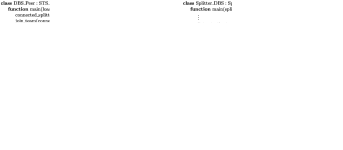
\includegraphics[width=\textwidth]{joining}
  \fig{1000}{10cm}{joining} \caption{Code related to team
    joining.\label{fig:joining}}
\end{figure*}

The new pseudo-code related to joining a team is describen in the
Fig.~\ref{fig:joining}.
\end{comment}

\begin{notex}
  See \href{https://github.com/P2PSP/simulator/blob/f0c73be1817e7d3b816cc61cd2c8e59b17f9a0e6/src/core/splitter_dbs.py#L296}{$\text{destination\_of\_chunk}[]$ in \texttt{peer\_dbs.py}}.
\end{notex}


\subsection{Buffering chunks}
%%% Local Variables:
%%% mode: latex
%%% TeX-master: "<none>"
%%% End:

\label{sec:buffering_chunks}

In order to hide the jitter generated by the physical network and the
protocol itself, peers need to store the received chunks in a buffer
during a period of time before playing them. A chunk with number $x$
is inserted in the position $(x \mathit{mod} 2B)$ of the buffer, where
$B$ is the maximum number of chunks that the buffer will store. In a
peer's life, $B$ is constant, but it is not compulsory that all peers
of the same team use the same $B$ value.

The buffer is implemented as a circular queue of $2B$ chunks, which is
filled up to only $B$ chunks in the buffering time (which is the main
part of the start-up time that the users experiment). Chunks with a
higher number (newer chunks) are inserted in the head of the
buffer. The chunk pointed by the tail of the buffer is sent to the
player (if there is a chunk in that cell of the buffer). This action
is carried out each time a new chunk is received.

Chunks can be lost.\footnote{Chunks are transmitted using a
  unrealiable communication, and therefore, network congestion can
  lose chunks.} A chunk is considered as lost when it is time to send
it to the player and the chunk has not been received.  In this
situation, for each lost chunk, the peer sends a $[\mathtt{request}
  \text{lost\_chunk\_number}]$ (that is the number of the next chunk
to be played) to the last neighbor served. When a peer $P_x$ receives
a $[\mathtt{request} \text{lost\_chunk\_number}]$ from $P_y$, $P_x$
adds $P_y$ to $\text{forward}[P_o]$, where $P_o$ is the origin peer of
the chunk stored in the position $lost\_chunk\_number$ of the buffer.

% As an alternative ...
\begin{comment}
origin peer of the next chunk stored in the
buffer. This peer has to characteristics: (1) it is not necessary a
neighbor peer, and (2) there is a high probability that this chunk has
been stored in the buffer ``for a long time'', so, if it is not a
neighbor, the link between it and the peer is working fairly well.
\end{comment}

\begin{notex}
  In the current implementation, the destination of the
  $[\mathtt{request} ...]$ message is the neighbor with the smaller
  chunk debt. This, a priori, has the drawback that this peer will
  always selected for relaying all the lost chunks because i will have
  a smaller debt as a consequence of the requests.
\end{notex}
  
In this situation, it is also possible that some peers can request
redundant paths between an origin peer and itself, and therefore, some
chunks could be received more than once. If this case, for each
duplicate chunk, a peer $P_i$ should send a $[\mathtt{prune}
  \text{duplicate\_chunk\_number}]$ message to those neighbors that
have sent to it the duplicate chunk. Neighbors receiving such message
from peer $P_i$ should remove the $P_i$ from $\text{forward}[P_o]$,
where $P_o$ is the origin peer of the duplicate chunk.

\begin{comment}
\begin{figure*}
  \fig{500}{5cm}{DBS_peer_buffering} \caption{Buffering of the
    chunks.\label{fig:DBS_peer_buffering}}
\end{figure*}
\end{comment}

The buffering time determines how much time the peers must wait before
start playing the chunks. Considering that chunks can be lost in
transit or delayed more than $B$ times of chunk, randomly, it is
difficult to determine, a priori the optimal buffering time. In the
current implementation, peers buffer a variable number of chunks that
depends on the order in which chunks are received. If $x_1$ is the
(number of the) first chunk received (the first chunk to be played),
the buffering time finishes when the chunk $x_1+B$ is
received.\footnote{Notice that all chunks with a number smaller than
  $x_1$ will be discarded, and that during the buffering time, it can
  happens that some chunks are not received on time. Therefore, it
  does not make sense to wait for $B$ chunks before stopping the
  buffering process.}

% Hablar de la relación entre B y el tamaño del team. Tal vez, cuando
% se presente la expresión de la latencia en función del grado de
% conectividad. En el caso extremo en que todos los peers se
% conectaran con todos, B >= N^*, el número máximo de peer en el team.

\begin{comment}
An heuristic that
works is the described in the Fig.~\ref{fig:DBS_peer_buffering}. As
can be seen, $\text{chunk\_to\_play}$ points to the first received
chunk, that not necessary is the received chunk with lower
index. After that, the
buffering finishes when a chunk with index $\text{chunk\_to\_play} +
\text{BUFFER\_SIZE}/2$ has been received.\footnote{This not means that
  $\text{BUFFER\_SIZE}/2$ chunks are available in the buffer.}
\end{comment}


\subsection{Chunk flooding}
\label{sec:chunk_flooding}
\begin{figure*}
  %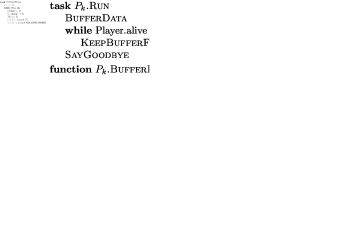
\includegraphics[width=0.75\textwidth]{chunk_generation_and_flooding}
  \fig{100}{3cm}{peer_chunk_flooding}
  \caption{Chunk flooding at peers.\label{fig:peer_chunk_flooding}}
\end{figure*}
When a peer $P_k$ receives a chunk from $P_i$, $P_k$ floods the
chunk to $T^k \setminus P_i$, using a prioritized round-robin
schema (see Fig.~\ref{fig:chunk_flooding}). Besides, if
it is a duplicate chunk, $P_k$ sends to $P_i$ a
$[\mathtt{NRFCF}~P_l]$ ($\mathtt{N}$ot $\mathtt{R}$elay
$\mathtt{F}$uture $\mathtt{C}$hunks $\mathtt{F}$rom) message, where
$P_l$ is the origin peer of the duplicate chunk. Thus, only
the first neighbor $P_i$ to send to $P_k$ a chunk
``originated'' at $P_l$ will do that in the future, at least
that $P_k$ revokes this routing information by sending a
$[\mathtt{RFCF}~P_l]$ ($\mathtt{R}$elay $\mathtt{F}$uture
$\mathtt{C}$hunks $\mathtt{F}$rom) to one or more (possibly the rest
of) peers of $T^k$.

As it has been said before, peers prioritize the flooding of the
chunks they relay by sending first the chunks to those neighbors that
are more supportive. To achieve that, every time $Pj_k$ sends a chunk
to $P_l$, $P_k$ runs $\mathtt{debt}[P_l] = \mathtt{debt}[P_l]+1$, and
$P_l$ runs $\mathtt{debt}[P_k] = \mathtt{debt}[P_k]-1$ (see
Fig.\ref{fig:}). Basically, these tables maintain a ``debt'' of chunks
between evey pair of neighbor peers. In ideal circunstances, debs
should be $0$. Debs are clipped to
$\pm\mathtt{debt}_{\text{max}}$. Obviously, a high supportivity means
a low debt, and viceversa.

\begin{comment}
In each round, peers check if a chunk have been received from the rest
of peers of the team (${\cal P}_k\in {\cal T}_j)$). If not, peers send
a $[\mathtt{propagate}~{\cal P}_i]$ to one or more (possibly
to the rest of) peers of the team, where ${\cal P}_i$ is the origin peer
of the missing chunk. At this point, the process continues as
described in Section~\ref{dbs:chunk_flooding}.
\end{comment}

\begin{comment}
For each ${\cal P}_k\in N({\cal P}_i)$, ${\cal P}_i$ checks if a chunk
has been received from ${\cal P}_k$. If ${\cal P}_i$ detects that
${\cal P}_k$ has not sent a chunk to it during $L$ consecutive rounds,
performs $N({\cal P}_i) = N({\cal P}_i)\setminus{\cal P}_k$, and stops
sending to ${\cal P}_k$ more chunks.
\end{comment}
\begin{comment}
computes a
``chunk-debt'', denoted by $d({\cal P}_k)$, that is incremented each
time a chunk is received from ${\cal P}_k$ and decremented each time a
chunk is sent to ${\cal P}_k$. If ${\cal P}_i$ verifies that $d({\cal
  P}_k)>D$ (the maximum debt), then ${\cal P}_i$ considers that ${\cal
  P}_k$ is unable to communicate with it, performs $N({\cal P}_i) =
N({\cal P}_i)\setminus{\cal P}_k$, and stops sending to ${\cal P}_k$
more chunks.
\end{comment}


%When peers receive chunks from their splitter, they must flood them to
%their neighbors until the chunks are broadcasted to the whole team
%(Fig.~\ref{fig:chunk_generation_and_flooding}). Lets suppose that
%${\cal P}_k$ receives a chunk. In the case the sender is its splitter,
%${\cal P}_k$ floods the chunk to $N({\cal P}_k)$. However, if the
%sender is a peer ${\cal P}_m\in N({\cal P}_k)$, ${\cal P}_k$ adds
%${\cal P}_m$ to $N({\cal P}_k)$ if ${\cal P}_m$ is a new neighbor, and
%forwards the chunk to the rest of its neighborhood ${\cal P}_n\in
%N({\cal P}_k)\setminus{\cal P}_m$ if ${\cal P}_k$ is in the shortest
%between ${\cal P}_n$ and the origin peer ${\cal P}_i$ of the relayed
%chunk. This will be true if ${\cal P}_k$ is the gateway of ${\cal
%  P}_n$ to go from ${\cal P}_n$ to ${\cal P}_i$. Therefore, a flooding
%with prunning based on shortest path routing is used.


\subsection{Routes discovery and topology optimization}
% Emacs, this is -*-latex-*-

% Routes Discovery and Topology Optimization

\label{sec:routes_discovery}

Chunks can be lost under bandwidth and buffering time constraints. A
chunk is lost when it is time to send it to the player, i.e. when it
is pointed by $p_p$, and the chunk has not been received. 
When a peer realizes that a chunk pointed by $p_p$ has been lost,
nothing can be done to recover it. Peers pre-fetch ``potentially
lost'' chunks at the buffer position $p_p+p_h$, where $p_h\geq 0$ is
the pre-feching horizon. Setting $p_h=0$, the pre-fetching is
disabled and only those chunks that really are lost will be
requested \leorem{no entiendo para que se piden}. 
On the contrary, the higher the $p_h$, the more aggressive
the pre-fetching is.  

For each (potentially) lost chunk with number
$\text{lost\_chunk\_number}$, peers send a
$[\mathtt{request}~\text{lost\_chunk\_number}]$ message to a random
peer of the team\leorem{solo uno? cuando se produce pruning?}. When a peer $P_i$ receives such message from 
$P_j$, $P_i$ adds $P_j$ to $\mathtt{forward}[P_k]$. $P_k$ is the
origin peer of the chunk stored in the position
$(\text{lost\_chunk\_number}~\mathit{mod}~2B)$ of $P_i$'s buffer in case this
chunks has been received. Otherwise, the request is ignored \leorem{y cómo se recupera?}. Notice
that, although request messages are very short, they are an overhead.

When request messages are used, redundant routes can be created and
therefore, some chunks could be received more than once. This is an overhead to be minimized. \leo{Upon the reception of the lost chunk, a peer send a pruning message to the other requested peers}. The receiver of the pruning message counts the number of times that a origin peer has been pruned, and when this counter is higher than a threshold $T$ (the maximum number of generated duplicates \leo{at requester's side}), the corresponding entry in the $\text{forward}[]$ table is deleted \leorem{Es por chunk o por origen?}.

Now, we can define more accurately the \gls{neighborhood-degree} (see
Sec.~\ref{sec:chunk_flooding}) as the number of different destination
peers for each possible origin that a peer forwards. For example, if a
peer $P_i$ forwards chunks from the origin $P_i$ to 10 neighbors, the
neighborhood degree of $P_i$ for the origin $P_i$ is 10, and if the
peer $P_i$ also forwards chunks from an origin $P_j$ to 5 neighbors,
the neighborhood degree of $P_i$ for the origin $P_j$ is 5\leorem{yo definiría dos tipos de grado de vecindad, el mio y el de reenvio}.

Considering the rules described before, the neighborhood degrees of
peers can decrease or increase to optimize the topology of the
overlay, by minimizing $\Delta t_b$. An increment in the degree for the origin of a requested
chunk $\text{lost\_chunk\_number}$ in $P_i$ is produced when $P_i$
recives a $[\mathtt{request}~\text{lost\_chunk\_number}]$ from a peer
that is not a neighbor, yet. On the contrary, a decrement in the
degree for the origin of a pruned chunk
$\text{duplicate\_chunk\_index}$ in $P_i$ is produced when $P_i$
receives a $[\mathtt{prune}~\text{duplicate\_chunk\_index}]$ from a
neighbor peer, for that origin. In fact, the continued use of the
requesting and pruning messages produce in a peer $P_i$ that the list
$\text{forward}[P_i]$ gets shorter (smaller \gls{neighborhood-degree})
and new entries in the table $\text{forward}[]$ are created.


%\subsection{Overlay topology optimization and the neighborhood degree}
%The neighborhood degree can also grow. When a chunk is lost, the peer
requests to receive the rest of chunks from the corresponding origin
peer to a random peer of the team. If duplicates are generated, prune
messages will remove the slower routes from that origin peer,
generating that the most reliable (and possiblely faster) route to
endure. When this happens, the requesting peer will be added to
$\mathtt{forward}[]$ (and therefore, sooner or later to
$\mathtt{pending}[]$) table of the requested peer, increasing its
neighborhood degree.


\subsection{Leaving a team}
\begin{figure*}
  %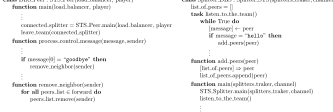
\includegraphics[width=0.55\textwidth]{leaving}
  \fig{300}{4cm}{leaving}
  \caption{Peer leaving.\label{fig:leaving}}
\end{figure*}
An outgoing peer $P^t_o$ (see Fig.~\ref{fig:leaving}) must to: (1) say
$[\mathtt{goodbye}]$ to $S^t$ and to $T^t_o$ (in this order), (2)
relay any pending (received but yet not sent) chunks, and (3) wait for
a $[\mathtt{goodbye}]$ from $S^t$, which performs $T^t = T^t \setminus
P^t_o$. In case of a timeout, $P^t_o$ resets the leaving procedure,
for a maximum number of times.

When a $P^t_k$ receives a $[\mathtt{goodbye}]$ from $P^t_o$, $P^t_k$
removes $P^t_o$ from its neighbors set, by running $T^t_k = T^t_k
\setminus P^t_o$.


\subsection{Free-riding control}
% Emacs, this is -*-latex-*-

% Free-riding Control at the Splitter

\label{sec:free_riding_control}

The splitter remembers which chunk, of a list of the last $B'$
transmitted chunks, was sent to each peer of the team. Notice that, in
order to remember the chunk that was sent to each peer in each round,
it must be hold that $B'\ge N$. \note{See
  \href{https://github.com/P2PSP/simulator/blob/f0c73be1817e7d3b816cc61cd2c8e59b17f9a0e6/src/core/splitter_dbs.py\#L296}{$\text{destination\_of\_chunk}[]$
    in \texttt{splitter\_dbs.py}}.}

Monitor peers (which are trusted peers) complain to their splitter
with a $[\mathtt{lost}~\text{lost\_chunk\_number}]$ for each lost
chunk. The splitter only considers these type of messages if they come
from a monitor.

%Notice that $L$ will
%tend to be proportional to the number $M$ of monitors, especially if
%those cases where $P_o$ is a gone peer that was unable to transmit the
%$[\mathtt{goodbye}]$ messages.

\begin{notex}
This last functionality has not been implemented, at least, as it has
been explained here. The forget() thread is controlled by a timer, not
by a counter of rounds.
\end{notex}

%Peers also control that at least one chunk is received from a neighbor
%in each round.\footnote{Peers recognize that a new round has started
%  when a new chunk is received from the splitter.} If happens that a
%peer $P_x$ does not receives a chunk from peer $P_y$ between $D^*$
%consecutive rounds, $P_x$ removes $P_y$ of its forwaring table.


%\subsection{Free-riding control at peers} % Neighborhood dynamics
%\label{dbs:frcp}
%Every time ${\cal P}^j_k$ sends a chunk to ${\cal P}^j_l$, ${\cal
P}^j_k$ runs $\mathtt{debt}[{\cal P}^j_l] = \mathtt{debt}[{\cal
P}^j_l]+1$, and ${\cal P}^j_l$ runs $\mathtt{debt}[{\cal P}^j_k]
= \mathtt{debt}[{\cal P}^j_k]-1$ (see Fig.\ref{fig}). Basically, these tables
maintain a ``debt'' of chunks between evey pair of neighbor
peers. If ${\cal P}^j_k$ realises that $\mathtt{debt}[{\cal
P}^j_l]>\mathtt{debt}_\text{max}$, then ${\cal P}^j_k$ removes ${\cal
P}^j_l$ from ${\cal T}^j_k$. Debts are clipped to $0$.

\begin{comment}
In each round, peers check if a chunk have been received from the rest
of peers of the team (${\cal P}_k\in {\cal T}_j)$). If not, peers send
a $[\mathtt{propagate}~{\cal P}_i]$ to one or more (possibly
to the rest of) peers of the team, where ${\cal P}_i$ is the origin peer
of the missing chunk. At this point, the process continues as
described in Section~\ref{dbs:chunk_flooding}.
\end{comment}

\begin{comment}
For each ${\cal P}_k\in N({\cal P}_i)$, ${\cal P}_i$ checks if a chunk
has been received from ${\cal P}_k$. If ${\cal P}_i$ detects that
${\cal P}_k$ has not sent a chunk to it during $L$ consecutive rounds,
performs $N({\cal P}_i) = N({\cal P}_i)\setminus{\cal P}_k$, and stops
sending to ${\cal P}_k$ more chunks.
\end{comment}
\begin{comment}
computes a
``chunk-debt'', denoted by $d({\cal P}_k)$, that is incremented each
time a chunk is received from ${\cal P}_k$ and decremented each time a
chunk is sent to ${\cal P}_k$. If ${\cal P}_i$ verifies that $d({\cal
  P}_k)>D$ (the maximum debt), then ${\cal P}_i$ considers that ${\cal
  P}_k$ is unable to communicate with it, performs $N({\cal P}_i) =
N({\cal P}_i)\setminus{\cal P}_k$, and stops sending to ${\cal P}_k$
more chunks.
\end{comment}


%\subsection{Congestion control}
%\label{dbs:congestion_control}
%P2PSP is a content-unaware push-based protocol. To avoid network
congestion while flooding, sending peers must perform some kind of
data flow-control. Moreover, to achieve aN ideal I/O ratio of $1$,
peers should send one chunk for every received one.

Congestion control in P2PSP is very simple: if a new chunk is
received, peers forward (using the flooding with prunning algorithm
described in Sec~\ref{dbs:chunk_generation_and_flooding}) each
received chunk to the next peer of their list of peers (following a
round-robin pattern).

%Peers do not understand the content, but it is
%known that in order to achieve a I/O ratio of 1, peers should send one
%chunk for every received one, on average. To acomplish this, a ${\cal
%  P}_i$ creates a FIFO queue of chunks for each $N({\cal P}_i)$, and,
%for each received chunk, ${\cal P}_i$ forwards a queued chunk from
%each of these queues.

\begin{comment}
A ${\cal P}_i$ forwards one or more chunks if and only if it has
received a chunk. For each received chunk $c_j$, ${\cal P}_i$: 1)
creates a list $l_{c_j}$ with the contents of $N'({\cal P}_i)$, and 2)
sends $c_j$ to $l_{c_j}[0]$ (the first element), and removes
$l_{c_j}[0]$. For each chunk reception, Step 2) is repeated for all
the previously created lists while they are not exhausted.

A solution is a forwarding algorithm based on the following
idea. Peers manage a list of chunks, where every item is a 2-tuple
($c_k$, $P_l$). The field $c_k$ represents the chunk that must be
flooded (if the node that has delivered the chunk is the splitter,
$c_k$ must be relayed towards all the neighbors, otherwise, $c_k$ must
be sent to all the neighbors except the peer that delivered $c_k$),
and the field $P_l$ the last neighbor to which $c_k$ was sent. For
every chunk received, a new tuple is appended to the list of chunks
and the rest of tuples are updated. The field $c_k$ remains constant
but $P_l$ is replaced by the next peer in the list of neighbors for
every received chunk.
\end{comment}


\begin{comment}
\subsubsection{Flooding order}
\label{dbs:flooding_order}
As an incentive mechanism~\cite{xu2006analysis}, peers relay received
chunks first to those peers that 
\end{comment}

%neighbors with lower chunk-debts.

\begin{comment}
\subsubsection{Team dynamics}
\label{dbs:team_dynamics}
${\cal P}_i$ adds to $N({\cal P}_i)$ those ${\cal P}_j$ that has sent
to ${\cal P}_i$ a chunk. If $N({\cal P}_i)>K$, periodically, ${\cal
  P}_i$ removes from $N({\cal P}_i)$ the peer with highest chunk-debt
and try to find in ${\cal T}_j\setminus N({\cal P}_i)$ a new peer using
$[\mathtt{hello}]$ messages.
\end{comment}

\begin{comment}
Peers use a buffer $b$ of chunks to hide the jitter generated by the
physical network and the broadcasting protocol. When a peer receives
$C_i$, it performs
\begin{equation}
  b[i~\text{mod}~B] = c_i,
\end{equation}
where ``mod'' represents the modulo operator and $B$ the buffer size
(in chunks). Basically, the buffer represents a sliding window that
moves over the stream synchronizely with the playing because the the
player consumes the chunks at the same chunk-rate the source produces
them.
\end{comment}

%%%%%%%%%%

\begin{comment}

\begin{itemize}

\item In the P2PSP, only monitor peers complains about lost
  chunks. This means that if a chunk that has been retransmitted by a
  peer is lost, it will be only retransmitted to all the peers of the
  team if the destination is a monitor peer and there is a unique
  monitor peer in the team. On the other hand, if the lost chunk was
  traveling from the splitter to a peer, all monitor peers will
  complain and this chunk will be retransmitted to the complete
  team. Therefore, only massively loss chunks will be retransmitted in
  the P2PSP. However, notice that a isolated missing chunk will
  produce negligible artifacts in the playback of one peer. In the
  Chain model, the lost of a chunk is handled between neighbour peers
  which means that all lost blocks should be, a priori, recovered.

\end{itemize}

\end{comment}



\begin{comment}
\subsubsection{Shortest path computation}
\label{dbs:chunk_routing}
\begin{figure}
  %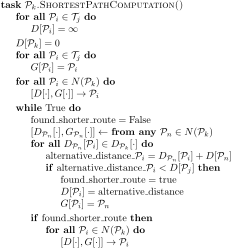
\includegraphics[width=0.35\textwidth]{shortest_path_computation}
  \fig{500}{4cm}{shortest_path_computation}
  \caption{Shortest path computation.\label{fig:shortest_path_computation}}
\end{figure}
The shortest path distances among peers are determined by a variation
of the Bellman-Ford Algorithm~\cite{Bertsekas1987data} (see
Fig.~\ref{fig:shortest_path_computation}), where the cost of the
``links'' between neighbor peers is $1$. Neighbor peers interchange
two vectors $D[\cdot]$ (distance-to-peer) and $G[\cdot]$
(gateway-to-peer) and compute the shortest distances and the (peer)
gateways to (reach) the rest of peers of its team ${\cal T}_j$.

This algorithm is free of routing loops and is not suceptible of the
well known count-to-infinity problem, and therefore always converges
for static teams. These problems do not appear because the routes are 

Each peer ${\cal P}_k$ sends
its vector of distances $D[\forall {\cal P}_i\in T^*({\cal P}_k)]$ and
gateways $G[\forall {\cal P}_i\in T^*({\cal P}_k)]$ to each
neighbor. When this information is received, peers check if shorter
routes can be found to the rest of peers of the reachable team, and if
so, send these vectors again.

The Bellman-Ford algorithm is susceptible of routing loops and the
count-to-infinite problem.


% Hace falta saber desde dónde viene el chunk original (origin peer) y que todos los peers dispongan de los vector-distances de los peers vecinos. Los vector-ditances deben tener tantas entradas como peers existen en el team. Por tanto, cada peer almacena un número de vector-distances igual a su grado de conectividad.


% Supposing that the weight of links between neighbors is 1.
% ¿Cómo sabe un peer que él es el último?
\end{comment}

\begin{comment}
\subsubsection{Generation of the routing tables}
Routing tables has as many entries as peers are in the team. The
routing table of a peer $P_i$ is a dictionary of pairs ($d(P_i, P_j)$,
$P_k$) indexed by the destination peer $P_j$ is a destination peer,
where $d(P_i, P_j)$ is the last measurement of the number of hops (in
peers) between $P_i$ and $P_j$, and $P_k\in N(P_i)$ is the 1-hop peer
that in the shortest-path between $P_i$ and $P_j$. Notice that if
$P_j==P_k$ then $d(P_i, P_j)==1$, which means that $P_i$ and $P_j$ are
directly ``connected''.

When a peer has updated its routing table, it is sent to their
neighbors pyggibacked on a \textsf{chunk} packet. When a peer receives
a routing table, it keeps a copy of it and updates its own routing
table with the new routing information using the Bellman-Ford
Algorithm~\cite{}. The peers have a copy of the routing table of its
neighbors to use it through the chunk routing process (see
Rule~\cite{the_routing_process}.
\end{comment}



\section{IMS (Ip Multicast Set)}
\label{sec:DBS}
DBS provides ALM for unicast (TCP/UDP) environments. The media is
received by a collection of
\emph{splitters} ${\cal S}=\{{\cal S}^0, \cdots, {\cal
  S}^{G-1}\}$ from a streaming server ${\cal O}$,
called \emph{source}, at a (usually variable) bit-rate which matches
the bit-rate of the media. Each ${\cal S}^i$ splits the
stream into a sequence of \emph{chunks}, and relay them to
different \emph{team} of up to $N$ \emph{peers}. We define the set of
teams as ${\cal T}=\{{\cal T}^0,\cdots,{\cal T}^{G-1}\}$ and the set
of peers per team $T^j=\{{\cal P}^j_0,\cdots,{\cal P}^j_{N-1}\}$.


%${\cal T}=\{{\cal T}_0,\cdots,{\cal T}_{G-1}\}$ \emph{teams} (one per
%  splitter) of up to $N$
%\emph{peers} $\{{\cal P}_0,\cdots,{\cal P}_{N-1}\}$, per team.


\subsection{Team definition and types of peers}
%%% Local Variables:
%%% mode: latex
%%% TeX-master: "<none>"
%%% End:

\label{sec:team_def}

A team is a set of one or more peers that share the same stream. By
definition, in a team of size one (the corresponding splitter is
considered out of the team if feeds), the only peer is known as a
\emph{monitor} peer, and in a team with more than one peer, at least
one of them must be a monitor peer. Monitors are instantiated by the
team administrator to monitorize different aspects of the
broadcasting, such as, the expected quality of the rendered video at
the peers or the expected average end-user latency.


\subsection{Feeding the team}
% Emacs, this is -*-latex-*-

% Feeding the Team

\label{sec:feeding_the_team}

The splitter divides the stream into chunks of constant length $C$,
and sends exclusively each chunk to a different
\gls{origin}\footnote{In the route that a chunk traces from the
  splitter to all peers of the team, the origin peer is the first one
  in this route i.e., the peer selected by the splitter for that
  chunk.}  peer, using a round-robin schema. Chunks are enumerated to
distinguish them, and this information is transmitted as a part of a chunk
header.

\begin{comment}
More details about the implementation
are available in Fig.~\ref{fig:chunk_generation}.

%$x$, conforming a message
%$c_x=[x,\text{chunk}]$, where
%$x=i \text{mod} \text{Splitter\_DBS.list\_of\_peers}.\text{length}()$.

\begin{figure*}
  %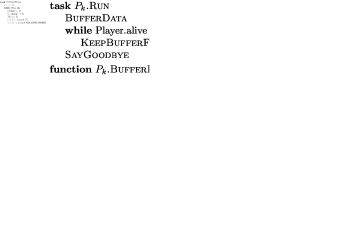
\includegraphics[width=0.75\textwidth]{chunk_generation_and_flooding}
  \fig{500}{5cm}{DBS_splitter_feed} \caption{Chunk
    generation at the splitter and their transmission to the
    team.\label{fig:chunk_generation}}
\end{figure*}
\end{comment}

A \gls{round} is defined as the process of transmitting $N$ different
chunks from the splitter to a team of $N\leq N^*$ peers (therefore,
all the peers of the team are origin of a different chunk, in each
round). For a team of size $N$, the average \gls{round-time} can be
estimated as
\begin{equation}
  t^{\mathrm{round}}=Nt^{\mathrm{chunk}},
\end{equation}
where $t^{\mathrm{chunk}}$ is the \gls{chunk-time}, defined as
\begin{equation}
  \label{eq:chunk_time}
  t^{\mathrm{chunk}}=\frac{l^{\mathrm{chunk}}}{R},
\end{equation}
where $l^{\mathrm{chunk}}$ is the length of the chunks (all the chunks are
split with the same length) and $R$ is the average transmission
bit-rate, that should match the average bit-rate of the stream in
order to achieve a seamsless playing.

\begin{comment}
The round-time is defined by:
\begin{equation}
  \cal{r} = \cal{c}N.
  \label{eq:round_time}
\end{equation}
For example, if we use only one team of $N=256$ peers, a chunk size
$C=1024$~bytes, and a video of $1$~Mb/s, the round time is
\begin{displaymath}
  \cal{r} = \frac{1024\frac{\text{bytes}}{\text{chunk}}\times
    8\frac{\text{bits}}{\text{byte}}}{10^6\frac{\text{bits}}{\text{second}}}\times
  256 \approx 2.1~\text{seconds}.
\end{displaymath}
\end{comment}


\subsection{Joining a team}
% Emacs, this is -*-latex-*-

% Joining the Team

\label{sec:joining}

After connecting with a splitter, incoming peers request (using a
reliable communication) to the splitter the current set of peers in
the team. To minimize the joining time, the peer sends a
$[\mathtt{hello}]$ message to each other peer of the team, in parallel
with the reception of the set. When a peer of the team receives a
$[\mathtt{hello}]$, it adds the sender of the message to a
\emph{table}\footnote{A structure which implements a random access
  efficiently.} of peers called $\mathtt{forward}[]$ \note{(see
  \href{https://github.com/P2PSP/simulator/blob/f0c73be1817e7d3b816cc61cd2c8e59b17f9a0e6/src/core/peer_dbs.py\#L491}{$\text{forward[]}$
    in \texttt{peer.py}})}. If a peer $P_i$ has an entry
$\mathtt{forward}[P_j]=P_k$, then each chunk received by $P_i$ and
originated at $P_j$ will be forwarded to $P_k$. When an incoming peer
$P_i$ has received the set of peers, its forwarding table has been
initialized to $\mathtt{forward}[P_i]=\{\text{team}\setminus
P_i\}$. Notice that, as long as the forwarding table contains this
information, all chunks received from the splitter will be forwarded
to the rest of the team, directly (in one protocol hop). So, in
absence of communication constraints, the team will be organized as a
full-connected overlay (see Fig.~\ref{fig:full_mesh}).

%), initializes
%the table $\mathrm{debt}[]$ (which stores the chunk debts between
%neighbor peers), and (3) sets the variable $\mathrm{neighbor}$ with an
%index to $\mathrm{forward}[]$ (see
%Sec.~\ref{sec:chunk_DBS_processing}).

The splitter, in an infinite loop: (1) listens to the incoming peers,
(2) sends to them the set of peers of the team, and (3) includes the
incoming peer to the set. Notice that only those peers that are in
the set of peers of the splitter are considered to be in the team
served by such splitter.

\begin{comment}
\begin{figure*}
  %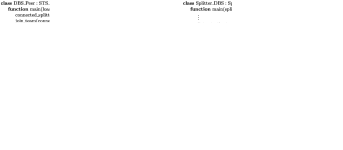
\includegraphics[width=\textwidth]{joining}
  \fig{1000}{10cm}{joining} \caption{Code related to team
    joining.\label{fig:joining}}
\end{figure*}

The new pseudo-code related to joining a team is describen in the
Fig.~\ref{fig:joining}.
\end{comment}

\begin{notex}
  See \href{https://github.com/P2PSP/simulator/blob/f0c73be1817e7d3b816cc61cd2c8e59b17f9a0e6/src/core/splitter_dbs.py#L296}{$\text{destination\_of\_chunk}[]$ in \texttt{peer\_dbs.py}}.
\end{notex}


\subsection{Buffering chunks}
%%% Local Variables:
%%% mode: latex
%%% TeX-master: "<none>"
%%% End:

\label{sec:buffering_chunks}

In order to hide the jitter generated by the physical network and the
protocol itself, peers need to store the received chunks in a buffer
during a period of time before playing them. A chunk with number $x$
is inserted in the position $(x \mathit{mod} 2B)$ of the buffer, where
$B$ is the maximum number of chunks that the buffer will store. In a
peer's life, $B$ is constant, but it is not compulsory that all peers
of the same team use the same $B$ value.

The buffer is implemented as a circular queue of $2B$ chunks, which is
filled up to only $B$ chunks in the buffering time (which is the main
part of the start-up time that the users experiment). Chunks with a
higher number (newer chunks) are inserted in the head of the
buffer. The chunk pointed by the tail of the buffer is sent to the
player (if there is a chunk in that cell of the buffer). This action
is carried out each time a new chunk is received.

Chunks can be lost.\footnote{Chunks are transmitted using a
  unrealiable communication, and therefore, network congestion can
  lose chunks.} A chunk is considered as lost when it is time to send
it to the player and the chunk has not been received.  In this
situation, for each lost chunk, the peer sends a $[\mathtt{request}
  \text{lost\_chunk\_number}]$ (that is the number of the next chunk
to be played) to the last neighbor served. When a peer $P_x$ receives
a $[\mathtt{request} \text{lost\_chunk\_number}]$ from $P_y$, $P_x$
adds $P_y$ to $\text{forward}[P_o]$, where $P_o$ is the origin peer of
the chunk stored in the position $lost\_chunk\_number$ of the buffer.

% As an alternative ...
\begin{comment}
origin peer of the next chunk stored in the
buffer. This peer has to characteristics: (1) it is not necessary a
neighbor peer, and (2) there is a high probability that this chunk has
been stored in the buffer ``for a long time'', so, if it is not a
neighbor, the link between it and the peer is working fairly well.
\end{comment}

\begin{notex}
  In the current implementation, the destination of the
  $[\mathtt{request} ...]$ message is the neighbor with the smaller
  chunk debt. This, a priori, has the drawback that this peer will
  always selected for relaying all the lost chunks because i will have
  a smaller debt as a consequence of the requests.
\end{notex}
  
In this situation, it is also possible that some peers can request
redundant paths between an origin peer and itself, and therefore, some
chunks could be received more than once. If this case, for each
duplicate chunk, a peer $P_i$ should send a $[\mathtt{prune}
  \text{duplicate\_chunk\_number}]$ message to those neighbors that
have sent to it the duplicate chunk. Neighbors receiving such message
from peer $P_i$ should remove the $P_i$ from $\text{forward}[P_o]$,
where $P_o$ is the origin peer of the duplicate chunk.

\begin{comment}
\begin{figure*}
  \fig{500}{5cm}{DBS_peer_buffering} \caption{Buffering of the
    chunks.\label{fig:DBS_peer_buffering}}
\end{figure*}
\end{comment}

The buffering time determines how much time the peers must wait before
start playing the chunks. Considering that chunks can be lost in
transit or delayed more than $B$ times of chunk, randomly, it is
difficult to determine, a priori the optimal buffering time. In the
current implementation, peers buffer a variable number of chunks that
depends on the order in which chunks are received. If $x_1$ is the
(number of the) first chunk received (the first chunk to be played),
the buffering time finishes when the chunk $x_1+B$ is
received.\footnote{Notice that all chunks with a number smaller than
  $x_1$ will be discarded, and that during the buffering time, it can
  happens that some chunks are not received on time. Therefore, it
  does not make sense to wait for $B$ chunks before stopping the
  buffering process.}

% Hablar de la relación entre B y el tamaño del team. Tal vez, cuando
% se presente la expresión de la latencia en función del grado de
% conectividad. En el caso extremo en que todos los peers se
% conectaran con todos, B >= N^*, el número máximo de peer en el team.

\begin{comment}
An heuristic that
works is the described in the Fig.~\ref{fig:DBS_peer_buffering}. As
can be seen, $\text{chunk\_to\_play}$ points to the first received
chunk, that not necessary is the received chunk with lower
index. After that, the
buffering finishes when a chunk with index $\text{chunk\_to\_play} +
\text{BUFFER\_SIZE}/2$ has been received.\footnote{This not means that
  $\text{BUFFER\_SIZE}/2$ chunks are available in the buffer.}
\end{comment}


\subsection{Chunk flooding}
\label{sec:chunk_flooding}
\begin{figure*}
  %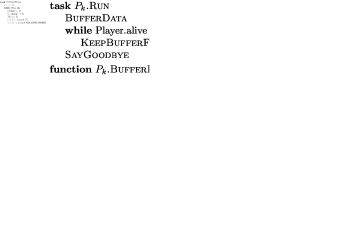
\includegraphics[width=0.75\textwidth]{chunk_generation_and_flooding}
  \fig{100}{3cm}{peer_chunk_flooding}
  \caption{Chunk flooding at peers.\label{fig:peer_chunk_flooding}}
\end{figure*}
When a peer $P_k$ receives a chunk from $P_i$, $P_k$ floods the
chunk to $T^k \setminus P_i$, using a prioritized round-robin
schema (see Fig.~\ref{fig:chunk_flooding}). Besides, if
it is a duplicate chunk, $P_k$ sends to $P_i$ a
$[\mathtt{NRFCF}~P_l]$ ($\mathtt{N}$ot $\mathtt{R}$elay
$\mathtt{F}$uture $\mathtt{C}$hunks $\mathtt{F}$rom) message, where
$P_l$ is the origin peer of the duplicate chunk. Thus, only
the first neighbor $P_i$ to send to $P_k$ a chunk
``originated'' at $P_l$ will do that in the future, at least
that $P_k$ revokes this routing information by sending a
$[\mathtt{RFCF}~P_l]$ ($\mathtt{R}$elay $\mathtt{F}$uture
$\mathtt{C}$hunks $\mathtt{F}$rom) to one or more (possibly the rest
of) peers of $T^k$.

As it has been said before, peers prioritize the flooding of the
chunks they relay by sending first the chunks to those neighbors that
are more supportive. To achieve that, every time $Pj_k$ sends a chunk
to $P_l$, $P_k$ runs $\mathtt{debt}[P_l] = \mathtt{debt}[P_l]+1$, and
$P_l$ runs $\mathtt{debt}[P_k] = \mathtt{debt}[P_k]-1$ (see
Fig.\ref{fig:}). Basically, these tables maintain a ``debt'' of chunks
between evey pair of neighbor peers. In ideal circunstances, debs
should be $0$. Debs are clipped to
$\pm\mathtt{debt}_{\text{max}}$. Obviously, a high supportivity means
a low debt, and viceversa.

\begin{comment}
In each round, peers check if a chunk have been received from the rest
of peers of the team (${\cal P}_k\in {\cal T}_j)$). If not, peers send
a $[\mathtt{propagate}~{\cal P}_i]$ to one or more (possibly
to the rest of) peers of the team, where ${\cal P}_i$ is the origin peer
of the missing chunk. At this point, the process continues as
described in Section~\ref{dbs:chunk_flooding}.
\end{comment}

\begin{comment}
For each ${\cal P}_k\in N({\cal P}_i)$, ${\cal P}_i$ checks if a chunk
has been received from ${\cal P}_k$. If ${\cal P}_i$ detects that
${\cal P}_k$ has not sent a chunk to it during $L$ consecutive rounds,
performs $N({\cal P}_i) = N({\cal P}_i)\setminus{\cal P}_k$, and stops
sending to ${\cal P}_k$ more chunks.
\end{comment}
\begin{comment}
computes a
``chunk-debt'', denoted by $d({\cal P}_k)$, that is incremented each
time a chunk is received from ${\cal P}_k$ and decremented each time a
chunk is sent to ${\cal P}_k$. If ${\cal P}_i$ verifies that $d({\cal
  P}_k)>D$ (the maximum debt), then ${\cal P}_i$ considers that ${\cal
  P}_k$ is unable to communicate with it, performs $N({\cal P}_i) =
N({\cal P}_i)\setminus{\cal P}_k$, and stops sending to ${\cal P}_k$
more chunks.
\end{comment}


%When peers receive chunks from their splitter, they must flood them to
%their neighbors until the chunks are broadcasted to the whole team
%(Fig.~\ref{fig:chunk_generation_and_flooding}). Lets suppose that
%${\cal P}_k$ receives a chunk. In the case the sender is its splitter,
%${\cal P}_k$ floods the chunk to $N({\cal P}_k)$. However, if the
%sender is a peer ${\cal P}_m\in N({\cal P}_k)$, ${\cal P}_k$ adds
%${\cal P}_m$ to $N({\cal P}_k)$ if ${\cal P}_m$ is a new neighbor, and
%forwards the chunk to the rest of its neighborhood ${\cal P}_n\in
%N({\cal P}_k)\setminus{\cal P}_m$ if ${\cal P}_k$ is in the shortest
%between ${\cal P}_n$ and the origin peer ${\cal P}_i$ of the relayed
%chunk. This will be true if ${\cal P}_k$ is the gateway of ${\cal
%  P}_n$ to go from ${\cal P}_n$ to ${\cal P}_i$. Therefore, a flooding
%with prunning based on shortest path routing is used.


\subsection{Routes discovery and topology optimization}
% Emacs, this is -*-latex-*-

% Routes Discovery and Topology Optimization

\label{sec:routes_discovery}

Chunks can be lost under bandwidth and buffering time constraints. A
chunk is lost when it is time to send it to the player, i.e. when it
is pointed by $p_p$, and the chunk has not been received. 
When a peer realizes that a chunk pointed by $p_p$ has been lost,
nothing can be done to recover it. Peers pre-fetch ``potentially
lost'' chunks at the buffer position $p_p+p_h$, where $p_h\geq 0$ is
the pre-feching horizon. Setting $p_h=0$, the pre-fetching is
disabled and only those chunks that really are lost will be
requested \leorem{no entiendo para que se piden}. 
On the contrary, the higher the $p_h$, the more aggressive
the pre-fetching is.  

For each (potentially) lost chunk with number
$\text{lost\_chunk\_number}$, peers send a
$[\mathtt{request}~\text{lost\_chunk\_number}]$ message to a random
peer of the team\leorem{solo uno? cuando se produce pruning?}. When a peer $P_i$ receives such message from 
$P_j$, $P_i$ adds $P_j$ to $\mathtt{forward}[P_k]$. $P_k$ is the
origin peer of the chunk stored in the position
$(\text{lost\_chunk\_number}~\mathit{mod}~2B)$ of $P_i$'s buffer in case this
chunks has been received. Otherwise, the request is ignored \leorem{y cómo se recupera?}. Notice
that, although request messages are very short, they are an overhead.

When request messages are used, redundant routes can be created and
therefore, some chunks could be received more than once. This is an overhead to be minimized. \leo{Upon the reception of the lost chunk, a peer send a pruning message to the other requested peers}. The receiver of the pruning message counts the number of times that a origin peer has been pruned, and when this counter is higher than a threshold $T$ (the maximum number of generated duplicates \leo{at requester's side}), the corresponding entry in the $\text{forward}[]$ table is deleted \leorem{Es por chunk o por origen?}.

Now, we can define more accurately the \gls{neighborhood-degree} (see
Sec.~\ref{sec:chunk_flooding}) as the number of different destination
peers for each possible origin that a peer forwards. For example, if a
peer $P_i$ forwards chunks from the origin $P_i$ to 10 neighbors, the
neighborhood degree of $P_i$ for the origin $P_i$ is 10, and if the
peer $P_i$ also forwards chunks from an origin $P_j$ to 5 neighbors,
the neighborhood degree of $P_i$ for the origin $P_j$ is 5\leorem{yo definiría dos tipos de grado de vecindad, el mio y el de reenvio}.

Considering the rules described before, the neighborhood degrees of
peers can decrease or increase to optimize the topology of the
overlay, by minimizing $\Delta t_b$. An increment in the degree for the origin of a requested
chunk $\text{lost\_chunk\_number}$ in $P_i$ is produced when $P_i$
recives a $[\mathtt{request}~\text{lost\_chunk\_number}]$ from a peer
that is not a neighbor, yet. On the contrary, a decrement in the
degree for the origin of a pruned chunk
$\text{duplicate\_chunk\_index}$ in $P_i$ is produced when $P_i$
receives a $[\mathtt{prune}~\text{duplicate\_chunk\_index}]$ from a
neighbor peer, for that origin. In fact, the continued use of the
requesting and pruning messages produce in a peer $P_i$ that the list
$\text{forward}[P_i]$ gets shorter (smaller \gls{neighborhood-degree})
and new entries in the table $\text{forward}[]$ are created.


%\subsection{Overlay topology optimization and the neighborhood degree}
%The neighborhood degree can also grow. When a chunk is lost, the peer
requests to receive the rest of chunks from the corresponding origin
peer to a random peer of the team. If duplicates are generated, prune
messages will remove the slower routes from that origin peer,
generating that the most reliable (and possiblely faster) route to
endure. When this happens, the requesting peer will be added to
$\mathtt{forward}[]$ (and therefore, sooner or later to
$\mathtt{pending}[]$) table of the requested peer, increasing its
neighborhood degree.


\subsection{Leaving a team}
\begin{figure*}
  %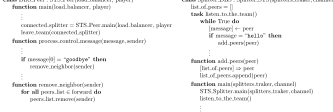
\includegraphics[width=0.55\textwidth]{leaving}
  \fig{300}{4cm}{leaving}
  \caption{Peer leaving.\label{fig:leaving}}
\end{figure*}
An outgoing peer $P^t_o$ (see Fig.~\ref{fig:leaving}) must to: (1) say
$[\mathtt{goodbye}]$ to $S^t$ and to $T^t_o$ (in this order), (2)
relay any pending (received but yet not sent) chunks, and (3) wait for
a $[\mathtt{goodbye}]$ from $S^t$, which performs $T^t = T^t \setminus
P^t_o$. In case of a timeout, $P^t_o$ resets the leaving procedure,
for a maximum number of times.

When a $P^t_k$ receives a $[\mathtt{goodbye}]$ from $P^t_o$, $P^t_k$
removes $P^t_o$ from its neighbors set, by running $T^t_k = T^t_k
\setminus P^t_o$.


\subsection{Free-riding control}
% Emacs, this is -*-latex-*-

% Free-riding Control at the Splitter

\label{sec:free_riding_control}

The splitter remembers which chunk, of a list of the last $B'$
transmitted chunks, was sent to each peer of the team. Notice that, in
order to remember the chunk that was sent to each peer in each round,
it must be hold that $B'\ge N$. \note{See
  \href{https://github.com/P2PSP/simulator/blob/f0c73be1817e7d3b816cc61cd2c8e59b17f9a0e6/src/core/splitter_dbs.py\#L296}{$\text{destination\_of\_chunk}[]$
    in \texttt{splitter\_dbs.py}}.}

Monitor peers (which are trusted peers) complain to their splitter
with a $[\mathtt{lost}~\text{lost\_chunk\_number}]$ for each lost
chunk. The splitter only considers these type of messages if they come
from a monitor.

%Notice that $L$ will
%tend to be proportional to the number $M$ of monitors, especially if
%those cases where $P_o$ is a gone peer that was unable to transmit the
%$[\mathtt{goodbye}]$ messages.

\begin{notex}
This last functionality has not been implemented, at least, as it has
been explained here. The forget() thread is controlled by a timer, not
by a counter of rounds.
\end{notex}

%Peers also control that at least one chunk is received from a neighbor
%in each round.\footnote{Peers recognize that a new round has started
%  when a new chunk is received from the splitter.} If happens that a
%peer $P_x$ does not receives a chunk from peer $P_y$ between $D^*$
%consecutive rounds, $P_x$ removes $P_y$ of its forwaring table.


%\subsection{Free-riding control at peers} % Neighborhood dynamics
%\label{dbs:frcp}
%Every time ${\cal P}^j_k$ sends a chunk to ${\cal P}^j_l$, ${\cal
P}^j_k$ runs $\mathtt{debt}[{\cal P}^j_l] = \mathtt{debt}[{\cal
P}^j_l]+1$, and ${\cal P}^j_l$ runs $\mathtt{debt}[{\cal P}^j_k]
= \mathtt{debt}[{\cal P}^j_k]-1$ (see Fig.\ref{fig}). Basically, these tables
maintain a ``debt'' of chunks between evey pair of neighbor
peers. If ${\cal P}^j_k$ realises that $\mathtt{debt}[{\cal
P}^j_l]>\mathtt{debt}_\text{max}$, then ${\cal P}^j_k$ removes ${\cal
P}^j_l$ from ${\cal T}^j_k$. Debts are clipped to $0$.

\begin{comment}
In each round, peers check if a chunk have been received from the rest
of peers of the team (${\cal P}_k\in {\cal T}_j)$). If not, peers send
a $[\mathtt{propagate}~{\cal P}_i]$ to one or more (possibly
to the rest of) peers of the team, where ${\cal P}_i$ is the origin peer
of the missing chunk. At this point, the process continues as
described in Section~\ref{dbs:chunk_flooding}.
\end{comment}

\begin{comment}
For each ${\cal P}_k\in N({\cal P}_i)$, ${\cal P}_i$ checks if a chunk
has been received from ${\cal P}_k$. If ${\cal P}_i$ detects that
${\cal P}_k$ has not sent a chunk to it during $L$ consecutive rounds,
performs $N({\cal P}_i) = N({\cal P}_i)\setminus{\cal P}_k$, and stops
sending to ${\cal P}_k$ more chunks.
\end{comment}
\begin{comment}
computes a
``chunk-debt'', denoted by $d({\cal P}_k)$, that is incremented each
time a chunk is received from ${\cal P}_k$ and decremented each time a
chunk is sent to ${\cal P}_k$. If ${\cal P}_i$ verifies that $d({\cal
  P}_k)>D$ (the maximum debt), then ${\cal P}_i$ considers that ${\cal
  P}_k$ is unable to communicate with it, performs $N({\cal P}_i) =
N({\cal P}_i)\setminus{\cal P}_k$, and stops sending to ${\cal P}_k$
more chunks.
\end{comment}


%\subsection{Congestion control}
%\label{dbs:congestion_control}
%P2PSP is a content-unaware push-based protocol. To avoid network
congestion while flooding, sending peers must perform some kind of
data flow-control. Moreover, to achieve aN ideal I/O ratio of $1$,
peers should send one chunk for every received one.

Congestion control in P2PSP is very simple: if a new chunk is
received, peers forward (using the flooding with prunning algorithm
described in Sec~\ref{dbs:chunk_generation_and_flooding}) each
received chunk to the next peer of their list of peers (following a
round-robin pattern).

%Peers do not understand the content, but it is
%known that in order to achieve a I/O ratio of 1, peers should send one
%chunk for every received one, on average. To acomplish this, a ${\cal
%  P}_i$ creates a FIFO queue of chunks for each $N({\cal P}_i)$, and,
%for each received chunk, ${\cal P}_i$ forwards a queued chunk from
%each of these queues.

\begin{comment}
A ${\cal P}_i$ forwards one or more chunks if and only if it has
received a chunk. For each received chunk $c_j$, ${\cal P}_i$: 1)
creates a list $l_{c_j}$ with the contents of $N'({\cal P}_i)$, and 2)
sends $c_j$ to $l_{c_j}[0]$ (the first element), and removes
$l_{c_j}[0]$. For each chunk reception, Step 2) is repeated for all
the previously created lists while they are not exhausted.

A solution is a forwarding algorithm based on the following
idea. Peers manage a list of chunks, where every item is a 2-tuple
($c_k$, $P_l$). The field $c_k$ represents the chunk that must be
flooded (if the node that has delivered the chunk is the splitter,
$c_k$ must be relayed towards all the neighbors, otherwise, $c_k$ must
be sent to all the neighbors except the peer that delivered $c_k$),
and the field $P_l$ the last neighbor to which $c_k$ was sent. For
every chunk received, a new tuple is appended to the list of chunks
and the rest of tuples are updated. The field $c_k$ remains constant
but $P_l$ is replaced by the next peer in the list of neighbors for
every received chunk.
\end{comment}


\begin{comment}
\subsubsection{Flooding order}
\label{dbs:flooding_order}
As an incentive mechanism~\cite{xu2006analysis}, peers relay received
chunks first to those peers that 
\end{comment}

%neighbors with lower chunk-debts.

\begin{comment}
\subsubsection{Team dynamics}
\label{dbs:team_dynamics}
${\cal P}_i$ adds to $N({\cal P}_i)$ those ${\cal P}_j$ that has sent
to ${\cal P}_i$ a chunk. If $N({\cal P}_i)>K$, periodically, ${\cal
  P}_i$ removes from $N({\cal P}_i)$ the peer with highest chunk-debt
and try to find in ${\cal T}_j\setminus N({\cal P}_i)$ a new peer using
$[\mathtt{hello}]$ messages.
\end{comment}

\begin{comment}
Peers use a buffer $b$ of chunks to hide the jitter generated by the
physical network and the broadcasting protocol. When a peer receives
$C_i$, it performs
\begin{equation}
  b[i~\text{mod}~B] = c_i,
\end{equation}
where ``mod'' represents the modulo operator and $B$ the buffer size
(in chunks). Basically, the buffer represents a sliding window that
moves over the stream synchronizely with the playing because the the
player consumes the chunks at the same chunk-rate the source produces
them.
\end{comment}

%%%%%%%%%%

\begin{comment}

\begin{itemize}

\item In the P2PSP, only monitor peers complains about lost
  chunks. This means that if a chunk that has been retransmitted by a
  peer is lost, it will be only retransmitted to all the peers of the
  team if the destination is a monitor peer and there is a unique
  monitor peer in the team. On the other hand, if the lost chunk was
  traveling from the splitter to a peer, all monitor peers will
  complain and this chunk will be retransmitted to the complete
  team. Therefore, only massively loss chunks will be retransmitted in
  the P2PSP. However, notice that a isolated missing chunk will
  produce negligible artifacts in the playback of one peer. In the
  Chain model, the lost of a chunk is handled between neighbour peers
  which means that all lost blocks should be, a priori, recovered.

\end{itemize}

\end{comment}



\begin{comment}
\subsubsection{Shortest path computation}
\label{dbs:chunk_routing}
\begin{figure}
  %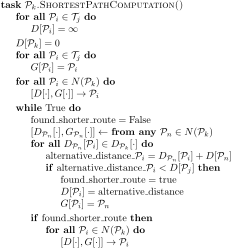
\includegraphics[width=0.35\textwidth]{shortest_path_computation}
  \fig{500}{4cm}{shortest_path_computation}
  \caption{Shortest path computation.\label{fig:shortest_path_computation}}
\end{figure}
The shortest path distances among peers are determined by a variation
of the Bellman-Ford Algorithm~\cite{Bertsekas1987data} (see
Fig.~\ref{fig:shortest_path_computation}), where the cost of the
``links'' between neighbor peers is $1$. Neighbor peers interchange
two vectors $D[\cdot]$ (distance-to-peer) and $G[\cdot]$
(gateway-to-peer) and compute the shortest distances and the (peer)
gateways to (reach) the rest of peers of its team ${\cal T}_j$.

This algorithm is free of routing loops and is not suceptible of the
well known count-to-infinity problem, and therefore always converges
for static teams. These problems do not appear because the routes are 

Each peer ${\cal P}_k$ sends
its vector of distances $D[\forall {\cal P}_i\in T^*({\cal P}_k)]$ and
gateways $G[\forall {\cal P}_i\in T^*({\cal P}_k)]$ to each
neighbor. When this information is received, peers check if shorter
routes can be found to the rest of peers of the reachable team, and if
so, send these vectors again.

The Bellman-Ford algorithm is susceptible of routing loops and the
count-to-infinite problem.


% Hace falta saber desde dónde viene el chunk original (origin peer) y que todos los peers dispongan de los vector-distances de los peers vecinos. Los vector-ditances deben tener tantas entradas como peers existen en el team. Por tanto, cada peer almacena un número de vector-distances igual a su grado de conectividad.


% Supposing that the weight of links between neighbors is 1.
% ¿Cómo sabe un peer que él es el último?
\end{comment}

\begin{comment}
\subsubsection{Generation of the routing tables}
Routing tables has as many entries as peers are in the team. The
routing table of a peer $P_i$ is a dictionary of pairs ($d(P_i, P_j)$,
$P_k$) indexed by the destination peer $P_j$ is a destination peer,
where $d(P_i, P_j)$ is the last measurement of the number of hops (in
peers) between $P_i$ and $P_j$, and $P_k\in N(P_i)$ is the 1-hop peer
that in the shortest-path between $P_i$ and $P_j$. Notice that if
$P_j==P_k$ then $d(P_i, P_j)==1$, which means that $P_i$ and $P_j$ are
directly ``connected''.

When a peer has updated its routing table, it is sent to their
neighbors pyggibacked on a \textsf{chunk} packet. When a peer receives
a routing table, it keeps a copy of it and updates its own routing
table with the new routing information using the Bellman-Ford
Algorithm~\cite{}. The peers have a copy of the routing table of its
neighbors to use it through the chunk routing process (see
Rule~\cite{the_routing_process}.
\end{comment}



\begin{comment}

\section{MRS (Massively-lost chunk Recovery Set)}
\label{sec:DBS}
DBS provides ALM for unicast (TCP/UDP) environments. The media is
received by a collection of
\emph{splitters} ${\cal S}=\{{\cal S}^0, \cdots, {\cal
  S}^{G-1}\}$ from a streaming server ${\cal O}$,
called \emph{source}, at a (usually variable) bit-rate which matches
the bit-rate of the media. Each ${\cal S}^i$ splits the
stream into a sequence of \emph{chunks}, and relay them to
different \emph{team} of up to $N$ \emph{peers}. We define the set of
teams as ${\cal T}=\{{\cal T}^0,\cdots,{\cal T}^{G-1}\}$ and the set
of peers per team $T^j=\{{\cal P}^j_0,\cdots,{\cal P}^j_{N-1}\}$.


%${\cal T}=\{{\cal T}_0,\cdots,{\cal T}_{G-1}\}$ \emph{teams} (one per
%  splitter) of up to $N$
%\emph{peers} $\{{\cal P}_0,\cdots,{\cal P}_{N-1}\}$, per team.


\subsection{Team definition and types of peers}
%%% Local Variables:
%%% mode: latex
%%% TeX-master: "<none>"
%%% End:

\label{sec:team_def}

A team is a set of one or more peers that share the same stream. By
definition, in a team of size one (the corresponding splitter is
considered out of the team if feeds), the only peer is known as a
\emph{monitor} peer, and in a team with more than one peer, at least
one of them must be a monitor peer. Monitors are instantiated by the
team administrator to monitorize different aspects of the
broadcasting, such as, the expected quality of the rendered video at
the peers or the expected average end-user latency.


\subsection{Feeding the team}
% Emacs, this is -*-latex-*-

% Feeding the Team

\label{sec:feeding_the_team}

The splitter divides the stream into chunks of constant length $C$,
and sends exclusively each chunk to a different
\gls{origin}\footnote{In the route that a chunk traces from the
  splitter to all peers of the team, the origin peer is the first one
  in this route i.e., the peer selected by the splitter for that
  chunk.}  peer, using a round-robin schema. Chunks are enumerated to
distinguish them, and this information is transmitted as a part of a chunk
header.

\begin{comment}
More details about the implementation
are available in Fig.~\ref{fig:chunk_generation}.

%$x$, conforming a message
%$c_x=[x,\text{chunk}]$, where
%$x=i \text{mod} \text{Splitter\_DBS.list\_of\_peers}.\text{length}()$.

\begin{figure*}
  %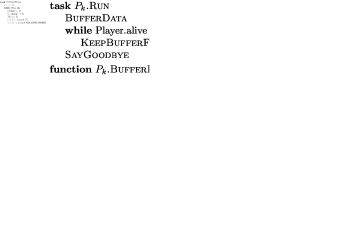
\includegraphics[width=0.75\textwidth]{chunk_generation_and_flooding}
  \fig{500}{5cm}{DBS_splitter_feed} \caption{Chunk
    generation at the splitter and their transmission to the
    team.\label{fig:chunk_generation}}
\end{figure*}
\end{comment}

A \gls{round} is defined as the process of transmitting $N$ different
chunks from the splitter to a team of $N\leq N^*$ peers (therefore,
all the peers of the team are origin of a different chunk, in each
round). For a team of size $N$, the average \gls{round-time} can be
estimated as
\begin{equation}
  t^{\mathrm{round}}=Nt^{\mathrm{chunk}},
\end{equation}
where $t^{\mathrm{chunk}}$ is the \gls{chunk-time}, defined as
\begin{equation}
  \label{eq:chunk_time}
  t^{\mathrm{chunk}}=\frac{l^{\mathrm{chunk}}}{R},
\end{equation}
where $l^{\mathrm{chunk}}$ is the length of the chunks (all the chunks are
split with the same length) and $R$ is the average transmission
bit-rate, that should match the average bit-rate of the stream in
order to achieve a seamsless playing.

\begin{comment}
The round-time is defined by:
\begin{equation}
  \cal{r} = \cal{c}N.
  \label{eq:round_time}
\end{equation}
For example, if we use only one team of $N=256$ peers, a chunk size
$C=1024$~bytes, and a video of $1$~Mb/s, the round time is
\begin{displaymath}
  \cal{r} = \frac{1024\frac{\text{bytes}}{\text{chunk}}\times
    8\frac{\text{bits}}{\text{byte}}}{10^6\frac{\text{bits}}{\text{second}}}\times
  256 \approx 2.1~\text{seconds}.
\end{displaymath}
\end{comment}


\subsection{Joining a team}
% Emacs, this is -*-latex-*-

% Joining the Team

\label{sec:joining}

After connecting with a splitter, incoming peers request (using a
reliable communication) to the splitter the current set of peers in
the team. To minimize the joining time, the peer sends a
$[\mathtt{hello}]$ message to each other peer of the team, in parallel
with the reception of the set. When a peer of the team receives a
$[\mathtt{hello}]$, it adds the sender of the message to a
\emph{table}\footnote{A structure which implements a random access
  efficiently.} of peers called $\mathtt{forward}[]$ \note{(see
  \href{https://github.com/P2PSP/simulator/blob/f0c73be1817e7d3b816cc61cd2c8e59b17f9a0e6/src/core/peer_dbs.py\#L491}{$\text{forward[]}$
    in \texttt{peer.py}})}. If a peer $P_i$ has an entry
$\mathtt{forward}[P_j]=P_k$, then each chunk received by $P_i$ and
originated at $P_j$ will be forwarded to $P_k$. When an incoming peer
$P_i$ has received the set of peers, its forwarding table has been
initialized to $\mathtt{forward}[P_i]=\{\text{team}\setminus
P_i\}$. Notice that, as long as the forwarding table contains this
information, all chunks received from the splitter will be forwarded
to the rest of the team, directly (in one protocol hop). So, in
absence of communication constraints, the team will be organized as a
full-connected overlay (see Fig.~\ref{fig:full_mesh}).

%), initializes
%the table $\mathrm{debt}[]$ (which stores the chunk debts between
%neighbor peers), and (3) sets the variable $\mathrm{neighbor}$ with an
%index to $\mathrm{forward}[]$ (see
%Sec.~\ref{sec:chunk_DBS_processing}).

The splitter, in an infinite loop: (1) listens to the incoming peers,
(2) sends to them the set of peers of the team, and (3) includes the
incoming peer to the set. Notice that only those peers that are in
the set of peers of the splitter are considered to be in the team
served by such splitter.

\begin{comment}
\begin{figure*}
  %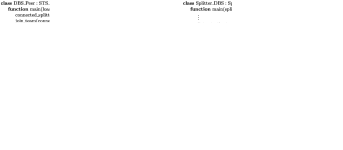
\includegraphics[width=\textwidth]{joining}
  \fig{1000}{10cm}{joining} \caption{Code related to team
    joining.\label{fig:joining}}
\end{figure*}

The new pseudo-code related to joining a team is describen in the
Fig.~\ref{fig:joining}.
\end{comment}

\begin{notex}
  See \href{https://github.com/P2PSP/simulator/blob/f0c73be1817e7d3b816cc61cd2c8e59b17f9a0e6/src/core/splitter_dbs.py#L296}{$\text{destination\_of\_chunk}[]$ in \texttt{peer\_dbs.py}}.
\end{notex}


\subsection{Buffering chunks}
%%% Local Variables:
%%% mode: latex
%%% TeX-master: "<none>"
%%% End:

\label{sec:buffering_chunks}

In order to hide the jitter generated by the physical network and the
protocol itself, peers need to store the received chunks in a buffer
during a period of time before playing them. A chunk with number $x$
is inserted in the position $(x \mathit{mod} 2B)$ of the buffer, where
$B$ is the maximum number of chunks that the buffer will store. In a
peer's life, $B$ is constant, but it is not compulsory that all peers
of the same team use the same $B$ value.

The buffer is implemented as a circular queue of $2B$ chunks, which is
filled up to only $B$ chunks in the buffering time (which is the main
part of the start-up time that the users experiment). Chunks with a
higher number (newer chunks) are inserted in the head of the
buffer. The chunk pointed by the tail of the buffer is sent to the
player (if there is a chunk in that cell of the buffer). This action
is carried out each time a new chunk is received.

Chunks can be lost.\footnote{Chunks are transmitted using a
  unrealiable communication, and therefore, network congestion can
  lose chunks.} A chunk is considered as lost when it is time to send
it to the player and the chunk has not been received.  In this
situation, for each lost chunk, the peer sends a $[\mathtt{request}
  \text{lost\_chunk\_number}]$ (that is the number of the next chunk
to be played) to the last neighbor served. When a peer $P_x$ receives
a $[\mathtt{request} \text{lost\_chunk\_number}]$ from $P_y$, $P_x$
adds $P_y$ to $\text{forward}[P_o]$, where $P_o$ is the origin peer of
the chunk stored in the position $lost\_chunk\_number$ of the buffer.

% As an alternative ...
\begin{comment}
origin peer of the next chunk stored in the
buffer. This peer has to characteristics: (1) it is not necessary a
neighbor peer, and (2) there is a high probability that this chunk has
been stored in the buffer ``for a long time'', so, if it is not a
neighbor, the link between it and the peer is working fairly well.
\end{comment}

\begin{notex}
  In the current implementation, the destination of the
  $[\mathtt{request} ...]$ message is the neighbor with the smaller
  chunk debt. This, a priori, has the drawback that this peer will
  always selected for relaying all the lost chunks because i will have
  a smaller debt as a consequence of the requests.
\end{notex}
  
In this situation, it is also possible that some peers can request
redundant paths between an origin peer and itself, and therefore, some
chunks could be received more than once. If this case, for each
duplicate chunk, a peer $P_i$ should send a $[\mathtt{prune}
  \text{duplicate\_chunk\_number}]$ message to those neighbors that
have sent to it the duplicate chunk. Neighbors receiving such message
from peer $P_i$ should remove the $P_i$ from $\text{forward}[P_o]$,
where $P_o$ is the origin peer of the duplicate chunk.

\begin{comment}
\begin{figure*}
  \fig{500}{5cm}{DBS_peer_buffering} \caption{Buffering of the
    chunks.\label{fig:DBS_peer_buffering}}
\end{figure*}
\end{comment}

The buffering time determines how much time the peers must wait before
start playing the chunks. Considering that chunks can be lost in
transit or delayed more than $B$ times of chunk, randomly, it is
difficult to determine, a priori the optimal buffering time. In the
current implementation, peers buffer a variable number of chunks that
depends on the order in which chunks are received. If $x_1$ is the
(number of the) first chunk received (the first chunk to be played),
the buffering time finishes when the chunk $x_1+B$ is
received.\footnote{Notice that all chunks with a number smaller than
  $x_1$ will be discarded, and that during the buffering time, it can
  happens that some chunks are not received on time. Therefore, it
  does not make sense to wait for $B$ chunks before stopping the
  buffering process.}

% Hablar de la relación entre B y el tamaño del team. Tal vez, cuando
% se presente la expresión de la latencia en función del grado de
% conectividad. En el caso extremo en que todos los peers se
% conectaran con todos, B >= N^*, el número máximo de peer en el team.

\begin{comment}
An heuristic that
works is the described in the Fig.~\ref{fig:DBS_peer_buffering}. As
can be seen, $\text{chunk\_to\_play}$ points to the first received
chunk, that not necessary is the received chunk with lower
index. After that, the
buffering finishes when a chunk with index $\text{chunk\_to\_play} +
\text{BUFFER\_SIZE}/2$ has been received.\footnote{This not means that
  $\text{BUFFER\_SIZE}/2$ chunks are available in the buffer.}
\end{comment}


\subsection{Chunk flooding}
\label{sec:chunk_flooding}
\begin{figure*}
  %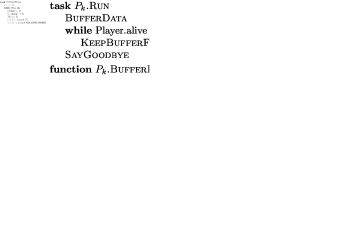
\includegraphics[width=0.75\textwidth]{chunk_generation_and_flooding}
  \fig{100}{3cm}{peer_chunk_flooding}
  \caption{Chunk flooding at peers.\label{fig:peer_chunk_flooding}}
\end{figure*}
When a peer $P_k$ receives a chunk from $P_i$, $P_k$ floods the
chunk to $T^k \setminus P_i$, using a prioritized round-robin
schema (see Fig.~\ref{fig:chunk_flooding}). Besides, if
it is a duplicate chunk, $P_k$ sends to $P_i$ a
$[\mathtt{NRFCF}~P_l]$ ($\mathtt{N}$ot $\mathtt{R}$elay
$\mathtt{F}$uture $\mathtt{C}$hunks $\mathtt{F}$rom) message, where
$P_l$ is the origin peer of the duplicate chunk. Thus, only
the first neighbor $P_i$ to send to $P_k$ a chunk
``originated'' at $P_l$ will do that in the future, at least
that $P_k$ revokes this routing information by sending a
$[\mathtt{RFCF}~P_l]$ ($\mathtt{R}$elay $\mathtt{F}$uture
$\mathtt{C}$hunks $\mathtt{F}$rom) to one or more (possibly the rest
of) peers of $T^k$.

As it has been said before, peers prioritize the flooding of the
chunks they relay by sending first the chunks to those neighbors that
are more supportive. To achieve that, every time $Pj_k$ sends a chunk
to $P_l$, $P_k$ runs $\mathtt{debt}[P_l] = \mathtt{debt}[P_l]+1$, and
$P_l$ runs $\mathtt{debt}[P_k] = \mathtt{debt}[P_k]-1$ (see
Fig.\ref{fig:}). Basically, these tables maintain a ``debt'' of chunks
between evey pair of neighbor peers. In ideal circunstances, debs
should be $0$. Debs are clipped to
$\pm\mathtt{debt}_{\text{max}}$. Obviously, a high supportivity means
a low debt, and viceversa.

\begin{comment}
In each round, peers check if a chunk have been received from the rest
of peers of the team (${\cal P}_k\in {\cal T}_j)$). If not, peers send
a $[\mathtt{propagate}~{\cal P}_i]$ to one or more (possibly
to the rest of) peers of the team, where ${\cal P}_i$ is the origin peer
of the missing chunk. At this point, the process continues as
described in Section~\ref{dbs:chunk_flooding}.
\end{comment}

\begin{comment}
For each ${\cal P}_k\in N({\cal P}_i)$, ${\cal P}_i$ checks if a chunk
has been received from ${\cal P}_k$. If ${\cal P}_i$ detects that
${\cal P}_k$ has not sent a chunk to it during $L$ consecutive rounds,
performs $N({\cal P}_i) = N({\cal P}_i)\setminus{\cal P}_k$, and stops
sending to ${\cal P}_k$ more chunks.
\end{comment}
\begin{comment}
computes a
``chunk-debt'', denoted by $d({\cal P}_k)$, that is incremented each
time a chunk is received from ${\cal P}_k$ and decremented each time a
chunk is sent to ${\cal P}_k$. If ${\cal P}_i$ verifies that $d({\cal
  P}_k)>D$ (the maximum debt), then ${\cal P}_i$ considers that ${\cal
  P}_k$ is unable to communicate with it, performs $N({\cal P}_i) =
N({\cal P}_i)\setminus{\cal P}_k$, and stops sending to ${\cal P}_k$
more chunks.
\end{comment}


%When peers receive chunks from their splitter, they must flood them to
%their neighbors until the chunks are broadcasted to the whole team
%(Fig.~\ref{fig:chunk_generation_and_flooding}). Lets suppose that
%${\cal P}_k$ receives a chunk. In the case the sender is its splitter,
%${\cal P}_k$ floods the chunk to $N({\cal P}_k)$. However, if the
%sender is a peer ${\cal P}_m\in N({\cal P}_k)$, ${\cal P}_k$ adds
%${\cal P}_m$ to $N({\cal P}_k)$ if ${\cal P}_m$ is a new neighbor, and
%forwards the chunk to the rest of its neighborhood ${\cal P}_n\in
%N({\cal P}_k)\setminus{\cal P}_m$ if ${\cal P}_k$ is in the shortest
%between ${\cal P}_n$ and the origin peer ${\cal P}_i$ of the relayed
%chunk. This will be true if ${\cal P}_k$ is the gateway of ${\cal
%  P}_n$ to go from ${\cal P}_n$ to ${\cal P}_i$. Therefore, a flooding
%with prunning based on shortest path routing is used.


\subsection{Routes discovery and topology optimization}
% Emacs, this is -*-latex-*-

% Routes Discovery and Topology Optimization

\label{sec:routes_discovery}

Chunks can be lost under bandwidth and buffering time constraints. A
chunk is lost when it is time to send it to the player, i.e. when it
is pointed by $p_p$, and the chunk has not been received. 
When a peer realizes that a chunk pointed by $p_p$ has been lost,
nothing can be done to recover it. Peers pre-fetch ``potentially
lost'' chunks at the buffer position $p_p+p_h$, where $p_h\geq 0$ is
the pre-feching horizon. Setting $p_h=0$, the pre-fetching is
disabled and only those chunks that really are lost will be
requested \leorem{no entiendo para que se piden}. 
On the contrary, the higher the $p_h$, the more aggressive
the pre-fetching is.  

For each (potentially) lost chunk with number
$\text{lost\_chunk\_number}$, peers send a
$[\mathtt{request}~\text{lost\_chunk\_number}]$ message to a random
peer of the team\leorem{solo uno? cuando se produce pruning?}. When a peer $P_i$ receives such message from 
$P_j$, $P_i$ adds $P_j$ to $\mathtt{forward}[P_k]$. $P_k$ is the
origin peer of the chunk stored in the position
$(\text{lost\_chunk\_number}~\mathit{mod}~2B)$ of $P_i$'s buffer in case this
chunks has been received. Otherwise, the request is ignored \leorem{y cómo se recupera?}. Notice
that, although request messages are very short, they are an overhead.

When request messages are used, redundant routes can be created and
therefore, some chunks could be received more than once. This is an overhead to be minimized. \leo{Upon the reception of the lost chunk, a peer send a pruning message to the other requested peers}. The receiver of the pruning message counts the number of times that a origin peer has been pruned, and when this counter is higher than a threshold $T$ (the maximum number of generated duplicates \leo{at requester's side}), the corresponding entry in the $\text{forward}[]$ table is deleted \leorem{Es por chunk o por origen?}.

Now, we can define more accurately the \gls{neighborhood-degree} (see
Sec.~\ref{sec:chunk_flooding}) as the number of different destination
peers for each possible origin that a peer forwards. For example, if a
peer $P_i$ forwards chunks from the origin $P_i$ to 10 neighbors, the
neighborhood degree of $P_i$ for the origin $P_i$ is 10, and if the
peer $P_i$ also forwards chunks from an origin $P_j$ to 5 neighbors,
the neighborhood degree of $P_i$ for the origin $P_j$ is 5\leorem{yo definiría dos tipos de grado de vecindad, el mio y el de reenvio}.

Considering the rules described before, the neighborhood degrees of
peers can decrease or increase to optimize the topology of the
overlay, by minimizing $\Delta t_b$. An increment in the degree for the origin of a requested
chunk $\text{lost\_chunk\_number}$ in $P_i$ is produced when $P_i$
recives a $[\mathtt{request}~\text{lost\_chunk\_number}]$ from a peer
that is not a neighbor, yet. On the contrary, a decrement in the
degree for the origin of a pruned chunk
$\text{duplicate\_chunk\_index}$ in $P_i$ is produced when $P_i$
receives a $[\mathtt{prune}~\text{duplicate\_chunk\_index}]$ from a
neighbor peer, for that origin. In fact, the continued use of the
requesting and pruning messages produce in a peer $P_i$ that the list
$\text{forward}[P_i]$ gets shorter (smaller \gls{neighborhood-degree})
and new entries in the table $\text{forward}[]$ are created.


%\subsection{Overlay topology optimization and the neighborhood degree}
%The neighborhood degree can also grow. When a chunk is lost, the peer
requests to receive the rest of chunks from the corresponding origin
peer to a random peer of the team. If duplicates are generated, prune
messages will remove the slower routes from that origin peer,
generating that the most reliable (and possiblely faster) route to
endure. When this happens, the requesting peer will be added to
$\mathtt{forward}[]$ (and therefore, sooner or later to
$\mathtt{pending}[]$) table of the requested peer, increasing its
neighborhood degree.


\subsection{Leaving a team}
\begin{figure*}
  %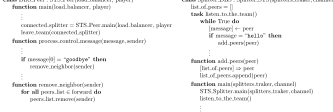
\includegraphics[width=0.55\textwidth]{leaving}
  \fig{300}{4cm}{leaving}
  \caption{Peer leaving.\label{fig:leaving}}
\end{figure*}
An outgoing peer $P^t_o$ (see Fig.~\ref{fig:leaving}) must to: (1) say
$[\mathtt{goodbye}]$ to $S^t$ and to $T^t_o$ (in this order), (2)
relay any pending (received but yet not sent) chunks, and (3) wait for
a $[\mathtt{goodbye}]$ from $S^t$, which performs $T^t = T^t \setminus
P^t_o$. In case of a timeout, $P^t_o$ resets the leaving procedure,
for a maximum number of times.

When a $P^t_k$ receives a $[\mathtt{goodbye}]$ from $P^t_o$, $P^t_k$
removes $P^t_o$ from its neighbors set, by running $T^t_k = T^t_k
\setminus P^t_o$.


\subsection{Free-riding control}
% Emacs, this is -*-latex-*-

% Free-riding Control at the Splitter

\label{sec:free_riding_control}

The splitter remembers which chunk, of a list of the last $B'$
transmitted chunks, was sent to each peer of the team. Notice that, in
order to remember the chunk that was sent to each peer in each round,
it must be hold that $B'\ge N$. \note{See
  \href{https://github.com/P2PSP/simulator/blob/f0c73be1817e7d3b816cc61cd2c8e59b17f9a0e6/src/core/splitter_dbs.py\#L296}{$\text{destination\_of\_chunk}[]$
    in \texttt{splitter\_dbs.py}}.}

Monitor peers (which are trusted peers) complain to their splitter
with a $[\mathtt{lost}~\text{lost\_chunk\_number}]$ for each lost
chunk. The splitter only considers these type of messages if they come
from a monitor.

%Notice that $L$ will
%tend to be proportional to the number $M$ of monitors, especially if
%those cases where $P_o$ is a gone peer that was unable to transmit the
%$[\mathtt{goodbye}]$ messages.

\begin{notex}
This last functionality has not been implemented, at least, as it has
been explained here. The forget() thread is controlled by a timer, not
by a counter of rounds.
\end{notex}

%Peers also control that at least one chunk is received from a neighbor
%in each round.\footnote{Peers recognize that a new round has started
%  when a new chunk is received from the splitter.} If happens that a
%peer $P_x$ does not receives a chunk from peer $P_y$ between $D^*$
%consecutive rounds, $P_x$ removes $P_y$ of its forwaring table.


%\subsection{Free-riding control at peers} % Neighborhood dynamics
%\label{dbs:frcp}
%Every time ${\cal P}^j_k$ sends a chunk to ${\cal P}^j_l$, ${\cal
P}^j_k$ runs $\mathtt{debt}[{\cal P}^j_l] = \mathtt{debt}[{\cal
P}^j_l]+1$, and ${\cal P}^j_l$ runs $\mathtt{debt}[{\cal P}^j_k]
= \mathtt{debt}[{\cal P}^j_k]-1$ (see Fig.\ref{fig}). Basically, these tables
maintain a ``debt'' of chunks between evey pair of neighbor
peers. If ${\cal P}^j_k$ realises that $\mathtt{debt}[{\cal
P}^j_l]>\mathtt{debt}_\text{max}$, then ${\cal P}^j_k$ removes ${\cal
P}^j_l$ from ${\cal T}^j_k$. Debts are clipped to $0$.

\begin{comment}
In each round, peers check if a chunk have been received from the rest
of peers of the team (${\cal P}_k\in {\cal T}_j)$). If not, peers send
a $[\mathtt{propagate}~{\cal P}_i]$ to one or more (possibly
to the rest of) peers of the team, where ${\cal P}_i$ is the origin peer
of the missing chunk. At this point, the process continues as
described in Section~\ref{dbs:chunk_flooding}.
\end{comment}

\begin{comment}
For each ${\cal P}_k\in N({\cal P}_i)$, ${\cal P}_i$ checks if a chunk
has been received from ${\cal P}_k$. If ${\cal P}_i$ detects that
${\cal P}_k$ has not sent a chunk to it during $L$ consecutive rounds,
performs $N({\cal P}_i) = N({\cal P}_i)\setminus{\cal P}_k$, and stops
sending to ${\cal P}_k$ more chunks.
\end{comment}
\begin{comment}
computes a
``chunk-debt'', denoted by $d({\cal P}_k)$, that is incremented each
time a chunk is received from ${\cal P}_k$ and decremented each time a
chunk is sent to ${\cal P}_k$. If ${\cal P}_i$ verifies that $d({\cal
  P}_k)>D$ (the maximum debt), then ${\cal P}_i$ considers that ${\cal
  P}_k$ is unable to communicate with it, performs $N({\cal P}_i) =
N({\cal P}_i)\setminus{\cal P}_k$, and stops sending to ${\cal P}_k$
more chunks.
\end{comment}


%\subsection{Congestion control}
%\label{dbs:congestion_control}
%P2PSP is a content-unaware push-based protocol. To avoid network
congestion while flooding, sending peers must perform some kind of
data flow-control. Moreover, to achieve aN ideal I/O ratio of $1$,
peers should send one chunk for every received one.

Congestion control in P2PSP is very simple: if a new chunk is
received, peers forward (using the flooding with prunning algorithm
described in Sec~\ref{dbs:chunk_generation_and_flooding}) each
received chunk to the next peer of their list of peers (following a
round-robin pattern).

%Peers do not understand the content, but it is
%known that in order to achieve a I/O ratio of 1, peers should send one
%chunk for every received one, on average. To acomplish this, a ${\cal
%  P}_i$ creates a FIFO queue of chunks for each $N({\cal P}_i)$, and,
%for each received chunk, ${\cal P}_i$ forwards a queued chunk from
%each of these queues.

\begin{comment}
A ${\cal P}_i$ forwards one or more chunks if and only if it has
received a chunk. For each received chunk $c_j$, ${\cal P}_i$: 1)
creates a list $l_{c_j}$ with the contents of $N'({\cal P}_i)$, and 2)
sends $c_j$ to $l_{c_j}[0]$ (the first element), and removes
$l_{c_j}[0]$. For each chunk reception, Step 2) is repeated for all
the previously created lists while they are not exhausted.

A solution is a forwarding algorithm based on the following
idea. Peers manage a list of chunks, where every item is a 2-tuple
($c_k$, $P_l$). The field $c_k$ represents the chunk that must be
flooded (if the node that has delivered the chunk is the splitter,
$c_k$ must be relayed towards all the neighbors, otherwise, $c_k$ must
be sent to all the neighbors except the peer that delivered $c_k$),
and the field $P_l$ the last neighbor to which $c_k$ was sent. For
every chunk received, a new tuple is appended to the list of chunks
and the rest of tuples are updated. The field $c_k$ remains constant
but $P_l$ is replaced by the next peer in the list of neighbors for
every received chunk.
\end{comment}


\begin{comment}
\subsubsection{Flooding order}
\label{dbs:flooding_order}
As an incentive mechanism~\cite{xu2006analysis}, peers relay received
chunks first to those peers that 
\end{comment}

%neighbors with lower chunk-debts.

\begin{comment}
\subsubsection{Team dynamics}
\label{dbs:team_dynamics}
${\cal P}_i$ adds to $N({\cal P}_i)$ those ${\cal P}_j$ that has sent
to ${\cal P}_i$ a chunk. If $N({\cal P}_i)>K$, periodically, ${\cal
  P}_i$ removes from $N({\cal P}_i)$ the peer with highest chunk-debt
and try to find in ${\cal T}_j\setminus N({\cal P}_i)$ a new peer using
$[\mathtt{hello}]$ messages.
\end{comment}

\begin{comment}
Peers use a buffer $b$ of chunks to hide the jitter generated by the
physical network and the broadcasting protocol. When a peer receives
$C_i$, it performs
\begin{equation}
  b[i~\text{mod}~B] = c_i,
\end{equation}
where ``mod'' represents the modulo operator and $B$ the buffer size
(in chunks). Basically, the buffer represents a sliding window that
moves over the stream synchronizely with the playing because the the
player consumes the chunks at the same chunk-rate the source produces
them.
\end{comment}

%%%%%%%%%%

\begin{comment}

\begin{itemize}

\item In the P2PSP, only monitor peers complains about lost
  chunks. This means that if a chunk that has been retransmitted by a
  peer is lost, it will be only retransmitted to all the peers of the
  team if the destination is a monitor peer and there is a unique
  monitor peer in the team. On the other hand, if the lost chunk was
  traveling from the splitter to a peer, all monitor peers will
  complain and this chunk will be retransmitted to the complete
  team. Therefore, only massively loss chunks will be retransmitted in
  the P2PSP. However, notice that a isolated missing chunk will
  produce negligible artifacts in the playback of one peer. In the
  Chain model, the lost of a chunk is handled between neighbour peers
  which means that all lost blocks should be, a priori, recovered.

\end{itemize}

\end{comment}



\begin{comment}
\subsubsection{Shortest path computation}
\label{dbs:chunk_routing}
\begin{figure}
  %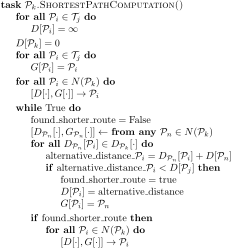
\includegraphics[width=0.35\textwidth]{shortest_path_computation}
  \fig{500}{4cm}{shortest_path_computation}
  \caption{Shortest path computation.\label{fig:shortest_path_computation}}
\end{figure}
The shortest path distances among peers are determined by a variation
of the Bellman-Ford Algorithm~\cite{Bertsekas1987data} (see
Fig.~\ref{fig:shortest_path_computation}), where the cost of the
``links'' between neighbor peers is $1$. Neighbor peers interchange
two vectors $D[\cdot]$ (distance-to-peer) and $G[\cdot]$
(gateway-to-peer) and compute the shortest distances and the (peer)
gateways to (reach) the rest of peers of its team ${\cal T}_j$.

This algorithm is free of routing loops and is not suceptible of the
well known count-to-infinity problem, and therefore always converges
for static teams. These problems do not appear because the routes are 

Each peer ${\cal P}_k$ sends
its vector of distances $D[\forall {\cal P}_i\in T^*({\cal P}_k)]$ and
gateways $G[\forall {\cal P}_i\in T^*({\cal P}_k)]$ to each
neighbor. When this information is received, peers check if shorter
routes can be found to the rest of peers of the reachable team, and if
so, send these vectors again.

The Bellman-Ford algorithm is susceptible of routing loops and the
count-to-infinite problem.


% Hace falta saber desde dónde viene el chunk original (origin peer) y que todos los peers dispongan de los vector-distances de los peers vecinos. Los vector-ditances deben tener tantas entradas como peers existen en el team. Por tanto, cada peer almacena un número de vector-distances igual a su grado de conectividad.


% Supposing that the weight of links between neighbors is 1.
% ¿Cómo sabe un peer que él es el último?
\end{comment}

\begin{comment}
\subsubsection{Generation of the routing tables}
Routing tables has as many entries as peers are in the team. The
routing table of a peer $P_i$ is a dictionary of pairs ($d(P_i, P_j)$,
$P_k$) indexed by the destination peer $P_j$ is a destination peer,
where $d(P_i, P_j)$ is the last measurement of the number of hops (in
peers) between $P_i$ and $P_j$, and $P_k\in N(P_i)$ is the 1-hop peer
that in the shortest-path between $P_i$ and $P_j$. Notice that if
$P_j==P_k$ then $d(P_i, P_j)==1$, which means that $P_i$ and $P_j$ are
directly ``connected''.

When a peer has updated its routing table, it is sent to their
neighbors pyggibacked on a \textsf{chunk} packet. When a peer receives
a routing table, it keeps a copy of it and updates its own routing
table with the new routing information using the Bellman-Ford
Algorithm~\cite{}. The peers have a copy of the routing table of its
neighbors to use it through the chunk routing process (see
Rule~\cite{the_routing_process}.
\end{comment}



\section{TAS (Topology Adaptation Set)}
\label{sec:DBS}
DBS provides ALM for unicast (TCP/UDP) environments. The media is
received by a collection of
\emph{splitters} ${\cal S}=\{{\cal S}^0, \cdots, {\cal
  S}^{G-1}\}$ from a streaming server ${\cal O}$,
called \emph{source}, at a (usually variable) bit-rate which matches
the bit-rate of the media. Each ${\cal S}^i$ splits the
stream into a sequence of \emph{chunks}, and relay them to
different \emph{team} of up to $N$ \emph{peers}. We define the set of
teams as ${\cal T}=\{{\cal T}^0,\cdots,{\cal T}^{G-1}\}$ and the set
of peers per team $T^j=\{{\cal P}^j_0,\cdots,{\cal P}^j_{N-1}\}$.


%${\cal T}=\{{\cal T}_0,\cdots,{\cal T}_{G-1}\}$ \emph{teams} (one per
%  splitter) of up to $N$
%\emph{peers} $\{{\cal P}_0,\cdots,{\cal P}_{N-1}\}$, per team.


\subsection{Team definition and types of peers}
%%% Local Variables:
%%% mode: latex
%%% TeX-master: "<none>"
%%% End:

\label{sec:team_def}

A team is a set of one or more peers that share the same stream. By
definition, in a team of size one (the corresponding splitter is
considered out of the team if feeds), the only peer is known as a
\emph{monitor} peer, and in a team with more than one peer, at least
one of them must be a monitor peer. Monitors are instantiated by the
team administrator to monitorize different aspects of the
broadcasting, such as, the expected quality of the rendered video at
the peers or the expected average end-user latency.


\subsection{Feeding the team}
% Emacs, this is -*-latex-*-

% Feeding the Team

\label{sec:feeding_the_team}

The splitter divides the stream into chunks of constant length $C$,
and sends exclusively each chunk to a different
\gls{origin}\footnote{In the route that a chunk traces from the
  splitter to all peers of the team, the origin peer is the first one
  in this route i.e., the peer selected by the splitter for that
  chunk.}  peer, using a round-robin schema. Chunks are enumerated to
distinguish them, and this information is transmitted as a part of a chunk
header.

\begin{comment}
More details about the implementation
are available in Fig.~\ref{fig:chunk_generation}.

%$x$, conforming a message
%$c_x=[x,\text{chunk}]$, where
%$x=i \text{mod} \text{Splitter\_DBS.list\_of\_peers}.\text{length}()$.

\begin{figure*}
  %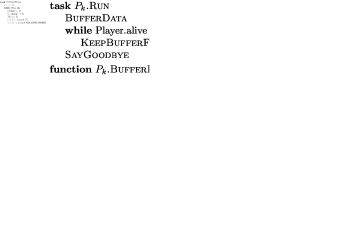
\includegraphics[width=0.75\textwidth]{chunk_generation_and_flooding}
  \fig{500}{5cm}{DBS_splitter_feed} \caption{Chunk
    generation at the splitter and their transmission to the
    team.\label{fig:chunk_generation}}
\end{figure*}
\end{comment}

A \gls{round} is defined as the process of transmitting $N$ different
chunks from the splitter to a team of $N\leq N^*$ peers (therefore,
all the peers of the team are origin of a different chunk, in each
round). For a team of size $N$, the average \gls{round-time} can be
estimated as
\begin{equation}
  t^{\mathrm{round}}=Nt^{\mathrm{chunk}},
\end{equation}
where $t^{\mathrm{chunk}}$ is the \gls{chunk-time}, defined as
\begin{equation}
  \label{eq:chunk_time}
  t^{\mathrm{chunk}}=\frac{l^{\mathrm{chunk}}}{R},
\end{equation}
where $l^{\mathrm{chunk}}$ is the length of the chunks (all the chunks are
split with the same length) and $R$ is the average transmission
bit-rate, that should match the average bit-rate of the stream in
order to achieve a seamsless playing.

\begin{comment}
The round-time is defined by:
\begin{equation}
  \cal{r} = \cal{c}N.
  \label{eq:round_time}
\end{equation}
For example, if we use only one team of $N=256$ peers, a chunk size
$C=1024$~bytes, and a video of $1$~Mb/s, the round time is
\begin{displaymath}
  \cal{r} = \frac{1024\frac{\text{bytes}}{\text{chunk}}\times
    8\frac{\text{bits}}{\text{byte}}}{10^6\frac{\text{bits}}{\text{second}}}\times
  256 \approx 2.1~\text{seconds}.
\end{displaymath}
\end{comment}


\subsection{Joining a team}
% Emacs, this is -*-latex-*-

% Joining the Team

\label{sec:joining}

After connecting with a splitter, incoming peers request (using a
reliable communication) to the splitter the current set of peers in
the team. To minimize the joining time, the peer sends a
$[\mathtt{hello}]$ message to each other peer of the team, in parallel
with the reception of the set. When a peer of the team receives a
$[\mathtt{hello}]$, it adds the sender of the message to a
\emph{table}\footnote{A structure which implements a random access
  efficiently.} of peers called $\mathtt{forward}[]$ \note{(see
  \href{https://github.com/P2PSP/simulator/blob/f0c73be1817e7d3b816cc61cd2c8e59b17f9a0e6/src/core/peer_dbs.py\#L491}{$\text{forward[]}$
    in \texttt{peer.py}})}. If a peer $P_i$ has an entry
$\mathtt{forward}[P_j]=P_k$, then each chunk received by $P_i$ and
originated at $P_j$ will be forwarded to $P_k$. When an incoming peer
$P_i$ has received the set of peers, its forwarding table has been
initialized to $\mathtt{forward}[P_i]=\{\text{team}\setminus
P_i\}$. Notice that, as long as the forwarding table contains this
information, all chunks received from the splitter will be forwarded
to the rest of the team, directly (in one protocol hop). So, in
absence of communication constraints, the team will be organized as a
full-connected overlay (see Fig.~\ref{fig:full_mesh}).

%), initializes
%the table $\mathrm{debt}[]$ (which stores the chunk debts between
%neighbor peers), and (3) sets the variable $\mathrm{neighbor}$ with an
%index to $\mathrm{forward}[]$ (see
%Sec.~\ref{sec:chunk_DBS_processing}).

The splitter, in an infinite loop: (1) listens to the incoming peers,
(2) sends to them the set of peers of the team, and (3) includes the
incoming peer to the set. Notice that only those peers that are in
the set of peers of the splitter are considered to be in the team
served by such splitter.

\begin{comment}
\begin{figure*}
  %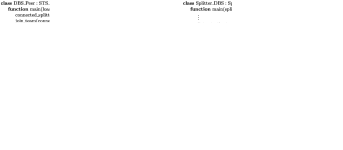
\includegraphics[width=\textwidth]{joining}
  \fig{1000}{10cm}{joining} \caption{Code related to team
    joining.\label{fig:joining}}
\end{figure*}

The new pseudo-code related to joining a team is describen in the
Fig.~\ref{fig:joining}.
\end{comment}

\begin{notex}
  See \href{https://github.com/P2PSP/simulator/blob/f0c73be1817e7d3b816cc61cd2c8e59b17f9a0e6/src/core/splitter_dbs.py#L296}{$\text{destination\_of\_chunk}[]$ in \texttt{peer\_dbs.py}}.
\end{notex}


\subsection{Buffering chunks}
%%% Local Variables:
%%% mode: latex
%%% TeX-master: "<none>"
%%% End:

\label{sec:buffering_chunks}

In order to hide the jitter generated by the physical network and the
protocol itself, peers need to store the received chunks in a buffer
during a period of time before playing them. A chunk with number $x$
is inserted in the position $(x \mathit{mod} 2B)$ of the buffer, where
$B$ is the maximum number of chunks that the buffer will store. In a
peer's life, $B$ is constant, but it is not compulsory that all peers
of the same team use the same $B$ value.

The buffer is implemented as a circular queue of $2B$ chunks, which is
filled up to only $B$ chunks in the buffering time (which is the main
part of the start-up time that the users experiment). Chunks with a
higher number (newer chunks) are inserted in the head of the
buffer. The chunk pointed by the tail of the buffer is sent to the
player (if there is a chunk in that cell of the buffer). This action
is carried out each time a new chunk is received.

Chunks can be lost.\footnote{Chunks are transmitted using a
  unrealiable communication, and therefore, network congestion can
  lose chunks.} A chunk is considered as lost when it is time to send
it to the player and the chunk has not been received.  In this
situation, for each lost chunk, the peer sends a $[\mathtt{request}
  \text{lost\_chunk\_number}]$ (that is the number of the next chunk
to be played) to the last neighbor served. When a peer $P_x$ receives
a $[\mathtt{request} \text{lost\_chunk\_number}]$ from $P_y$, $P_x$
adds $P_y$ to $\text{forward}[P_o]$, where $P_o$ is the origin peer of
the chunk stored in the position $lost\_chunk\_number$ of the buffer.

% As an alternative ...
\begin{comment}
origin peer of the next chunk stored in the
buffer. This peer has to characteristics: (1) it is not necessary a
neighbor peer, and (2) there is a high probability that this chunk has
been stored in the buffer ``for a long time'', so, if it is not a
neighbor, the link between it and the peer is working fairly well.
\end{comment}

\begin{notex}
  In the current implementation, the destination of the
  $[\mathtt{request} ...]$ message is the neighbor with the smaller
  chunk debt. This, a priori, has the drawback that this peer will
  always selected for relaying all the lost chunks because i will have
  a smaller debt as a consequence of the requests.
\end{notex}
  
In this situation, it is also possible that some peers can request
redundant paths between an origin peer and itself, and therefore, some
chunks could be received more than once. If this case, for each
duplicate chunk, a peer $P_i$ should send a $[\mathtt{prune}
  \text{duplicate\_chunk\_number}]$ message to those neighbors that
have sent to it the duplicate chunk. Neighbors receiving such message
from peer $P_i$ should remove the $P_i$ from $\text{forward}[P_o]$,
where $P_o$ is the origin peer of the duplicate chunk.

\begin{comment}
\begin{figure*}
  \fig{500}{5cm}{DBS_peer_buffering} \caption{Buffering of the
    chunks.\label{fig:DBS_peer_buffering}}
\end{figure*}
\end{comment}

The buffering time determines how much time the peers must wait before
start playing the chunks. Considering that chunks can be lost in
transit or delayed more than $B$ times of chunk, randomly, it is
difficult to determine, a priori the optimal buffering time. In the
current implementation, peers buffer a variable number of chunks that
depends on the order in which chunks are received. If $x_1$ is the
(number of the) first chunk received (the first chunk to be played),
the buffering time finishes when the chunk $x_1+B$ is
received.\footnote{Notice that all chunks with a number smaller than
  $x_1$ will be discarded, and that during the buffering time, it can
  happens that some chunks are not received on time. Therefore, it
  does not make sense to wait for $B$ chunks before stopping the
  buffering process.}

% Hablar de la relación entre B y el tamaño del team. Tal vez, cuando
% se presente la expresión de la latencia en función del grado de
% conectividad. En el caso extremo en que todos los peers se
% conectaran con todos, B >= N^*, el número máximo de peer en el team.

\begin{comment}
An heuristic that
works is the described in the Fig.~\ref{fig:DBS_peer_buffering}. As
can be seen, $\text{chunk\_to\_play}$ points to the first received
chunk, that not necessary is the received chunk with lower
index. After that, the
buffering finishes when a chunk with index $\text{chunk\_to\_play} +
\text{BUFFER\_SIZE}/2$ has been received.\footnote{This not means that
  $\text{BUFFER\_SIZE}/2$ chunks are available in the buffer.}
\end{comment}


\subsection{Chunk flooding}
\label{sec:chunk_flooding}
\begin{figure*}
  %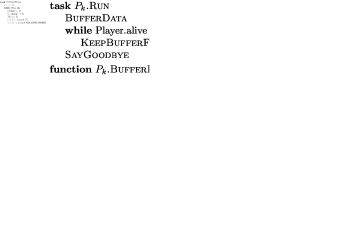
\includegraphics[width=0.75\textwidth]{chunk_generation_and_flooding}
  \fig{100}{3cm}{peer_chunk_flooding}
  \caption{Chunk flooding at peers.\label{fig:peer_chunk_flooding}}
\end{figure*}
When a peer $P_k$ receives a chunk from $P_i$, $P_k$ floods the
chunk to $T^k \setminus P_i$, using a prioritized round-robin
schema (see Fig.~\ref{fig:chunk_flooding}). Besides, if
it is a duplicate chunk, $P_k$ sends to $P_i$ a
$[\mathtt{NRFCF}~P_l]$ ($\mathtt{N}$ot $\mathtt{R}$elay
$\mathtt{F}$uture $\mathtt{C}$hunks $\mathtt{F}$rom) message, where
$P_l$ is the origin peer of the duplicate chunk. Thus, only
the first neighbor $P_i$ to send to $P_k$ a chunk
``originated'' at $P_l$ will do that in the future, at least
that $P_k$ revokes this routing information by sending a
$[\mathtt{RFCF}~P_l]$ ($\mathtt{R}$elay $\mathtt{F}$uture
$\mathtt{C}$hunks $\mathtt{F}$rom) to one or more (possibly the rest
of) peers of $T^k$.

As it has been said before, peers prioritize the flooding of the
chunks they relay by sending first the chunks to those neighbors that
are more supportive. To achieve that, every time $Pj_k$ sends a chunk
to $P_l$, $P_k$ runs $\mathtt{debt}[P_l] = \mathtt{debt}[P_l]+1$, and
$P_l$ runs $\mathtt{debt}[P_k] = \mathtt{debt}[P_k]-1$ (see
Fig.\ref{fig:}). Basically, these tables maintain a ``debt'' of chunks
between evey pair of neighbor peers. In ideal circunstances, debs
should be $0$. Debs are clipped to
$\pm\mathtt{debt}_{\text{max}}$. Obviously, a high supportivity means
a low debt, and viceversa.

\begin{comment}
In each round, peers check if a chunk have been received from the rest
of peers of the team (${\cal P}_k\in {\cal T}_j)$). If not, peers send
a $[\mathtt{propagate}~{\cal P}_i]$ to one or more (possibly
to the rest of) peers of the team, where ${\cal P}_i$ is the origin peer
of the missing chunk. At this point, the process continues as
described in Section~\ref{dbs:chunk_flooding}.
\end{comment}

\begin{comment}
For each ${\cal P}_k\in N({\cal P}_i)$, ${\cal P}_i$ checks if a chunk
has been received from ${\cal P}_k$. If ${\cal P}_i$ detects that
${\cal P}_k$ has not sent a chunk to it during $L$ consecutive rounds,
performs $N({\cal P}_i) = N({\cal P}_i)\setminus{\cal P}_k$, and stops
sending to ${\cal P}_k$ more chunks.
\end{comment}
\begin{comment}
computes a
``chunk-debt'', denoted by $d({\cal P}_k)$, that is incremented each
time a chunk is received from ${\cal P}_k$ and decremented each time a
chunk is sent to ${\cal P}_k$. If ${\cal P}_i$ verifies that $d({\cal
  P}_k)>D$ (the maximum debt), then ${\cal P}_i$ considers that ${\cal
  P}_k$ is unable to communicate with it, performs $N({\cal P}_i) =
N({\cal P}_i)\setminus{\cal P}_k$, and stops sending to ${\cal P}_k$
more chunks.
\end{comment}


%When peers receive chunks from their splitter, they must flood them to
%their neighbors until the chunks are broadcasted to the whole team
%(Fig.~\ref{fig:chunk_generation_and_flooding}). Lets suppose that
%${\cal P}_k$ receives a chunk. In the case the sender is its splitter,
%${\cal P}_k$ floods the chunk to $N({\cal P}_k)$. However, if the
%sender is a peer ${\cal P}_m\in N({\cal P}_k)$, ${\cal P}_k$ adds
%${\cal P}_m$ to $N({\cal P}_k)$ if ${\cal P}_m$ is a new neighbor, and
%forwards the chunk to the rest of its neighborhood ${\cal P}_n\in
%N({\cal P}_k)\setminus{\cal P}_m$ if ${\cal P}_k$ is in the shortest
%between ${\cal P}_n$ and the origin peer ${\cal P}_i$ of the relayed
%chunk. This will be true if ${\cal P}_k$ is the gateway of ${\cal
%  P}_n$ to go from ${\cal P}_n$ to ${\cal P}_i$. Therefore, a flooding
%with prunning based on shortest path routing is used.


\subsection{Routes discovery and topology optimization}
% Emacs, this is -*-latex-*-

% Routes Discovery and Topology Optimization

\label{sec:routes_discovery}

Chunks can be lost under bandwidth and buffering time constraints. A
chunk is lost when it is time to send it to the player, i.e. when it
is pointed by $p_p$, and the chunk has not been received. 
When a peer realizes that a chunk pointed by $p_p$ has been lost,
nothing can be done to recover it. Peers pre-fetch ``potentially
lost'' chunks at the buffer position $p_p+p_h$, where $p_h\geq 0$ is
the pre-feching horizon. Setting $p_h=0$, the pre-fetching is
disabled and only those chunks that really are lost will be
requested \leorem{no entiendo para que se piden}. 
On the contrary, the higher the $p_h$, the more aggressive
the pre-fetching is.  

For each (potentially) lost chunk with number
$\text{lost\_chunk\_number}$, peers send a
$[\mathtt{request}~\text{lost\_chunk\_number}]$ message to a random
peer of the team\leorem{solo uno? cuando se produce pruning?}. When a peer $P_i$ receives such message from 
$P_j$, $P_i$ adds $P_j$ to $\mathtt{forward}[P_k]$. $P_k$ is the
origin peer of the chunk stored in the position
$(\text{lost\_chunk\_number}~\mathit{mod}~2B)$ of $P_i$'s buffer in case this
chunks has been received. Otherwise, the request is ignored \leorem{y cómo se recupera?}. Notice
that, although request messages are very short, they are an overhead.

When request messages are used, redundant routes can be created and
therefore, some chunks could be received more than once. This is an overhead to be minimized. \leo{Upon the reception of the lost chunk, a peer send a pruning message to the other requested peers}. The receiver of the pruning message counts the number of times that a origin peer has been pruned, and when this counter is higher than a threshold $T$ (the maximum number of generated duplicates \leo{at requester's side}), the corresponding entry in the $\text{forward}[]$ table is deleted \leorem{Es por chunk o por origen?}.

Now, we can define more accurately the \gls{neighborhood-degree} (see
Sec.~\ref{sec:chunk_flooding}) as the number of different destination
peers for each possible origin that a peer forwards. For example, if a
peer $P_i$ forwards chunks from the origin $P_i$ to 10 neighbors, the
neighborhood degree of $P_i$ for the origin $P_i$ is 10, and if the
peer $P_i$ also forwards chunks from an origin $P_j$ to 5 neighbors,
the neighborhood degree of $P_i$ for the origin $P_j$ is 5\leorem{yo definiría dos tipos de grado de vecindad, el mio y el de reenvio}.

Considering the rules described before, the neighborhood degrees of
peers can decrease or increase to optimize the topology of the
overlay, by minimizing $\Delta t_b$. An increment in the degree for the origin of a requested
chunk $\text{lost\_chunk\_number}$ in $P_i$ is produced when $P_i$
recives a $[\mathtt{request}~\text{lost\_chunk\_number}]$ from a peer
that is not a neighbor, yet. On the contrary, a decrement in the
degree for the origin of a pruned chunk
$\text{duplicate\_chunk\_index}$ in $P_i$ is produced when $P_i$
receives a $[\mathtt{prune}~\text{duplicate\_chunk\_index}]$ from a
neighbor peer, for that origin. In fact, the continued use of the
requesting and pruning messages produce in a peer $P_i$ that the list
$\text{forward}[P_i]$ gets shorter (smaller \gls{neighborhood-degree})
and new entries in the table $\text{forward}[]$ are created.


%\subsection{Overlay topology optimization and the neighborhood degree}
%The neighborhood degree can also grow. When a chunk is lost, the peer
requests to receive the rest of chunks from the corresponding origin
peer to a random peer of the team. If duplicates are generated, prune
messages will remove the slower routes from that origin peer,
generating that the most reliable (and possiblely faster) route to
endure. When this happens, the requesting peer will be added to
$\mathtt{forward}[]$ (and therefore, sooner or later to
$\mathtt{pending}[]$) table of the requested peer, increasing its
neighborhood degree.


\subsection{Leaving a team}
\begin{figure*}
  %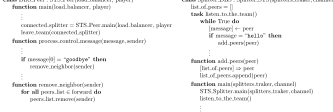
\includegraphics[width=0.55\textwidth]{leaving}
  \fig{300}{4cm}{leaving}
  \caption{Peer leaving.\label{fig:leaving}}
\end{figure*}
An outgoing peer $P^t_o$ (see Fig.~\ref{fig:leaving}) must to: (1) say
$[\mathtt{goodbye}]$ to $S^t$ and to $T^t_o$ (in this order), (2)
relay any pending (received but yet not sent) chunks, and (3) wait for
a $[\mathtt{goodbye}]$ from $S^t$, which performs $T^t = T^t \setminus
P^t_o$. In case of a timeout, $P^t_o$ resets the leaving procedure,
for a maximum number of times.

When a $P^t_k$ receives a $[\mathtt{goodbye}]$ from $P^t_o$, $P^t_k$
removes $P^t_o$ from its neighbors set, by running $T^t_k = T^t_k
\setminus P^t_o$.


\subsection{Free-riding control}
% Emacs, this is -*-latex-*-

% Free-riding Control at the Splitter

\label{sec:free_riding_control}

The splitter remembers which chunk, of a list of the last $B'$
transmitted chunks, was sent to each peer of the team. Notice that, in
order to remember the chunk that was sent to each peer in each round,
it must be hold that $B'\ge N$. \note{See
  \href{https://github.com/P2PSP/simulator/blob/f0c73be1817e7d3b816cc61cd2c8e59b17f9a0e6/src/core/splitter_dbs.py\#L296}{$\text{destination\_of\_chunk}[]$
    in \texttt{splitter\_dbs.py}}.}

Monitor peers (which are trusted peers) complain to their splitter
with a $[\mathtt{lost}~\text{lost\_chunk\_number}]$ for each lost
chunk. The splitter only considers these type of messages if they come
from a monitor.

%Notice that $L$ will
%tend to be proportional to the number $M$ of monitors, especially if
%those cases where $P_o$ is a gone peer that was unable to transmit the
%$[\mathtt{goodbye}]$ messages.

\begin{notex}
This last functionality has not been implemented, at least, as it has
been explained here. The forget() thread is controlled by a timer, not
by a counter of rounds.
\end{notex}

%Peers also control that at least one chunk is received from a neighbor
%in each round.\footnote{Peers recognize that a new round has started
%  when a new chunk is received from the splitter.} If happens that a
%peer $P_x$ does not receives a chunk from peer $P_y$ between $D^*$
%consecutive rounds, $P_x$ removes $P_y$ of its forwaring table.


%\subsection{Free-riding control at peers} % Neighborhood dynamics
%\label{dbs:frcp}
%Every time ${\cal P}^j_k$ sends a chunk to ${\cal P}^j_l$, ${\cal
P}^j_k$ runs $\mathtt{debt}[{\cal P}^j_l] = \mathtt{debt}[{\cal
P}^j_l]+1$, and ${\cal P}^j_l$ runs $\mathtt{debt}[{\cal P}^j_k]
= \mathtt{debt}[{\cal P}^j_k]-1$ (see Fig.\ref{fig}). Basically, these tables
maintain a ``debt'' of chunks between evey pair of neighbor
peers. If ${\cal P}^j_k$ realises that $\mathtt{debt}[{\cal
P}^j_l]>\mathtt{debt}_\text{max}$, then ${\cal P}^j_k$ removes ${\cal
P}^j_l$ from ${\cal T}^j_k$. Debts are clipped to $0$.

\begin{comment}
In each round, peers check if a chunk have been received from the rest
of peers of the team (${\cal P}_k\in {\cal T}_j)$). If not, peers send
a $[\mathtt{propagate}~{\cal P}_i]$ to one or more (possibly
to the rest of) peers of the team, where ${\cal P}_i$ is the origin peer
of the missing chunk. At this point, the process continues as
described in Section~\ref{dbs:chunk_flooding}.
\end{comment}

\begin{comment}
For each ${\cal P}_k\in N({\cal P}_i)$, ${\cal P}_i$ checks if a chunk
has been received from ${\cal P}_k$. If ${\cal P}_i$ detects that
${\cal P}_k$ has not sent a chunk to it during $L$ consecutive rounds,
performs $N({\cal P}_i) = N({\cal P}_i)\setminus{\cal P}_k$, and stops
sending to ${\cal P}_k$ more chunks.
\end{comment}
\begin{comment}
computes a
``chunk-debt'', denoted by $d({\cal P}_k)$, that is incremented each
time a chunk is received from ${\cal P}_k$ and decremented each time a
chunk is sent to ${\cal P}_k$. If ${\cal P}_i$ verifies that $d({\cal
  P}_k)>D$ (the maximum debt), then ${\cal P}_i$ considers that ${\cal
  P}_k$ is unable to communicate with it, performs $N({\cal P}_i) =
N({\cal P}_i)\setminus{\cal P}_k$, and stops sending to ${\cal P}_k$
more chunks.
\end{comment}


%\subsection{Congestion control}
%\label{dbs:congestion_control}
%P2PSP is a content-unaware push-based protocol. To avoid network
congestion while flooding, sending peers must perform some kind of
data flow-control. Moreover, to achieve aN ideal I/O ratio of $1$,
peers should send one chunk for every received one.

Congestion control in P2PSP is very simple: if a new chunk is
received, peers forward (using the flooding with prunning algorithm
described in Sec~\ref{dbs:chunk_generation_and_flooding}) each
received chunk to the next peer of their list of peers (following a
round-robin pattern).

%Peers do not understand the content, but it is
%known that in order to achieve a I/O ratio of 1, peers should send one
%chunk for every received one, on average. To acomplish this, a ${\cal
%  P}_i$ creates a FIFO queue of chunks for each $N({\cal P}_i)$, and,
%for each received chunk, ${\cal P}_i$ forwards a queued chunk from
%each of these queues.

\begin{comment}
A ${\cal P}_i$ forwards one or more chunks if and only if it has
received a chunk. For each received chunk $c_j$, ${\cal P}_i$: 1)
creates a list $l_{c_j}$ with the contents of $N'({\cal P}_i)$, and 2)
sends $c_j$ to $l_{c_j}[0]$ (the first element), and removes
$l_{c_j}[0]$. For each chunk reception, Step 2) is repeated for all
the previously created lists while they are not exhausted.

A solution is a forwarding algorithm based on the following
idea. Peers manage a list of chunks, where every item is a 2-tuple
($c_k$, $P_l$). The field $c_k$ represents the chunk that must be
flooded (if the node that has delivered the chunk is the splitter,
$c_k$ must be relayed towards all the neighbors, otherwise, $c_k$ must
be sent to all the neighbors except the peer that delivered $c_k$),
and the field $P_l$ the last neighbor to which $c_k$ was sent. For
every chunk received, a new tuple is appended to the list of chunks
and the rest of tuples are updated. The field $c_k$ remains constant
but $P_l$ is replaced by the next peer in the list of neighbors for
every received chunk.
\end{comment}


\begin{comment}
\subsubsection{Flooding order}
\label{dbs:flooding_order}
As an incentive mechanism~\cite{xu2006analysis}, peers relay received
chunks first to those peers that 
\end{comment}

%neighbors with lower chunk-debts.

\begin{comment}
\subsubsection{Team dynamics}
\label{dbs:team_dynamics}
${\cal P}_i$ adds to $N({\cal P}_i)$ those ${\cal P}_j$ that has sent
to ${\cal P}_i$ a chunk. If $N({\cal P}_i)>K$, periodically, ${\cal
  P}_i$ removes from $N({\cal P}_i)$ the peer with highest chunk-debt
and try to find in ${\cal T}_j\setminus N({\cal P}_i)$ a new peer using
$[\mathtt{hello}]$ messages.
\end{comment}

\begin{comment}
Peers use a buffer $b$ of chunks to hide the jitter generated by the
physical network and the broadcasting protocol. When a peer receives
$C_i$, it performs
\begin{equation}
  b[i~\text{mod}~B] = c_i,
\end{equation}
where ``mod'' represents the modulo operator and $B$ the buffer size
(in chunks). Basically, the buffer represents a sliding window that
moves over the stream synchronizely with the playing because the the
player consumes the chunks at the same chunk-rate the source produces
them.
\end{comment}

%%%%%%%%%%

\begin{comment}

\begin{itemize}

\item In the P2PSP, only monitor peers complains about lost
  chunks. This means that if a chunk that has been retransmitted by a
  peer is lost, it will be only retransmitted to all the peers of the
  team if the destination is a monitor peer and there is a unique
  monitor peer in the team. On the other hand, if the lost chunk was
  traveling from the splitter to a peer, all monitor peers will
  complain and this chunk will be retransmitted to the complete
  team. Therefore, only massively loss chunks will be retransmitted in
  the P2PSP. However, notice that a isolated missing chunk will
  produce negligible artifacts in the playback of one peer. In the
  Chain model, the lost of a chunk is handled between neighbour peers
  which means that all lost blocks should be, a priori, recovered.

\end{itemize}

\end{comment}



\begin{comment}
\subsubsection{Shortest path computation}
\label{dbs:chunk_routing}
\begin{figure}
  %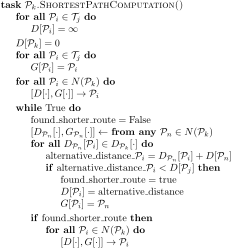
\includegraphics[width=0.35\textwidth]{shortest_path_computation}
  \fig{500}{4cm}{shortest_path_computation}
  \caption{Shortest path computation.\label{fig:shortest_path_computation}}
\end{figure}
The shortest path distances among peers are determined by a variation
of the Bellman-Ford Algorithm~\cite{Bertsekas1987data} (see
Fig.~\ref{fig:shortest_path_computation}), where the cost of the
``links'' between neighbor peers is $1$. Neighbor peers interchange
two vectors $D[\cdot]$ (distance-to-peer) and $G[\cdot]$
(gateway-to-peer) and compute the shortest distances and the (peer)
gateways to (reach) the rest of peers of its team ${\cal T}_j$.

This algorithm is free of routing loops and is not suceptible of the
well known count-to-infinity problem, and therefore always converges
for static teams. These problems do not appear because the routes are 

Each peer ${\cal P}_k$ sends
its vector of distances $D[\forall {\cal P}_i\in T^*({\cal P}_k)]$ and
gateways $G[\forall {\cal P}_i\in T^*({\cal P}_k)]$ to each
neighbor. When this information is received, peers check if shorter
routes can be found to the rest of peers of the reachable team, and if
so, send these vectors again.

The Bellman-Ford algorithm is susceptible of routing loops and the
count-to-infinite problem.


% Hace falta saber desde dónde viene el chunk original (origin peer) y que todos los peers dispongan de los vector-distances de los peers vecinos. Los vector-ditances deben tener tantas entradas como peers existen en el team. Por tanto, cada peer almacena un número de vector-distances igual a su grado de conectividad.


% Supposing that the weight of links between neighbors is 1.
% ¿Cómo sabe un peer que él es el último?
\end{comment}

\begin{comment}
\subsubsection{Generation of the routing tables}
Routing tables has as many entries as peers are in the team. The
routing table of a peer $P_i$ is a dictionary of pairs ($d(P_i, P_j)$,
$P_k$) indexed by the destination peer $P_j$ is a destination peer,
where $d(P_i, P_j)$ is the last measurement of the number of hops (in
peers) between $P_i$ and $P_j$, and $P_k\in N(P_i)$ is the 1-hop peer
that in the shortest-path between $P_i$ and $P_j$. Notice that if
$P_j==P_k$ then $d(P_i, P_j)==1$, which means that $P_i$ and $P_j$ are
directly ``connected''.

When a peer has updated its routing table, it is sent to their
neighbors pyggibacked on a \textsf{chunk} packet. When a peer receives
a routing table, it keeps a copy of it and updates its own routing
table with the new routing information using the Bellman-Ford
Algorithm~\cite{}. The peers have a copy of the routing table of its
neighbors to use it through the chunk routing process (see
Rule~\cite{the_routing_process}.
\end{comment}



\section{ACS (Adaptive Capacity Set)}
\label{sec:DBS}
DBS provides ALM for unicast (TCP/UDP) environments. The media is
received by a collection of
\emph{splitters} ${\cal S}=\{{\cal S}^0, \cdots, {\cal
  S}^{G-1}\}$ from a streaming server ${\cal O}$,
called \emph{source}, at a (usually variable) bit-rate which matches
the bit-rate of the media. Each ${\cal S}^i$ splits the
stream into a sequence of \emph{chunks}, and relay them to
different \emph{team} of up to $N$ \emph{peers}. We define the set of
teams as ${\cal T}=\{{\cal T}^0,\cdots,{\cal T}^{G-1}\}$ and the set
of peers per team $T^j=\{{\cal P}^j_0,\cdots,{\cal P}^j_{N-1}\}$.


%${\cal T}=\{{\cal T}_0,\cdots,{\cal T}_{G-1}\}$ \emph{teams} (one per
%  splitter) of up to $N$
%\emph{peers} $\{{\cal P}_0,\cdots,{\cal P}_{N-1}\}$, per team.


\subsection{Team definition and types of peers}
%%% Local Variables:
%%% mode: latex
%%% TeX-master: "<none>"
%%% End:

\label{sec:team_def}

A team is a set of one or more peers that share the same stream. By
definition, in a team of size one (the corresponding splitter is
considered out of the team if feeds), the only peer is known as a
\emph{monitor} peer, and in a team with more than one peer, at least
one of them must be a monitor peer. Monitors are instantiated by the
team administrator to monitorize different aspects of the
broadcasting, such as, the expected quality of the rendered video at
the peers or the expected average end-user latency.


\subsection{Feeding the team}
% Emacs, this is -*-latex-*-

% Feeding the Team

\label{sec:feeding_the_team}

The splitter divides the stream into chunks of constant length $C$,
and sends exclusively each chunk to a different
\gls{origin}\footnote{In the route that a chunk traces from the
  splitter to all peers of the team, the origin peer is the first one
  in this route i.e., the peer selected by the splitter for that
  chunk.}  peer, using a round-robin schema. Chunks are enumerated to
distinguish them, and this information is transmitted as a part of a chunk
header.

\begin{comment}
More details about the implementation
are available in Fig.~\ref{fig:chunk_generation}.

%$x$, conforming a message
%$c_x=[x,\text{chunk}]$, where
%$x=i \text{mod} \text{Splitter\_DBS.list\_of\_peers}.\text{length}()$.

\begin{figure*}
  %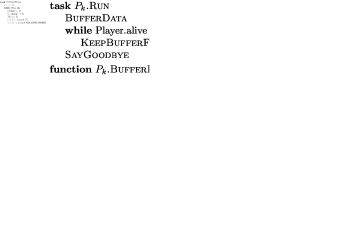
\includegraphics[width=0.75\textwidth]{chunk_generation_and_flooding}
  \fig{500}{5cm}{DBS_splitter_feed} \caption{Chunk
    generation at the splitter and their transmission to the
    team.\label{fig:chunk_generation}}
\end{figure*}
\end{comment}

A \gls{round} is defined as the process of transmitting $N$ different
chunks from the splitter to a team of $N\leq N^*$ peers (therefore,
all the peers of the team are origin of a different chunk, in each
round). For a team of size $N$, the average \gls{round-time} can be
estimated as
\begin{equation}
  t^{\mathrm{round}}=Nt^{\mathrm{chunk}},
\end{equation}
where $t^{\mathrm{chunk}}$ is the \gls{chunk-time}, defined as
\begin{equation}
  \label{eq:chunk_time}
  t^{\mathrm{chunk}}=\frac{l^{\mathrm{chunk}}}{R},
\end{equation}
where $l^{\mathrm{chunk}}$ is the length of the chunks (all the chunks are
split with the same length) and $R$ is the average transmission
bit-rate, that should match the average bit-rate of the stream in
order to achieve a seamsless playing.

\begin{comment}
The round-time is defined by:
\begin{equation}
  \cal{r} = \cal{c}N.
  \label{eq:round_time}
\end{equation}
For example, if we use only one team of $N=256$ peers, a chunk size
$C=1024$~bytes, and a video of $1$~Mb/s, the round time is
\begin{displaymath}
  \cal{r} = \frac{1024\frac{\text{bytes}}{\text{chunk}}\times
    8\frac{\text{bits}}{\text{byte}}}{10^6\frac{\text{bits}}{\text{second}}}\times
  256 \approx 2.1~\text{seconds}.
\end{displaymath}
\end{comment}


\subsection{Joining a team}
% Emacs, this is -*-latex-*-

% Joining the Team

\label{sec:joining}

After connecting with a splitter, incoming peers request (using a
reliable communication) to the splitter the current set of peers in
the team. To minimize the joining time, the peer sends a
$[\mathtt{hello}]$ message to each other peer of the team, in parallel
with the reception of the set. When a peer of the team receives a
$[\mathtt{hello}]$, it adds the sender of the message to a
\emph{table}\footnote{A structure which implements a random access
  efficiently.} of peers called $\mathtt{forward}[]$ \note{(see
  \href{https://github.com/P2PSP/simulator/blob/f0c73be1817e7d3b816cc61cd2c8e59b17f9a0e6/src/core/peer_dbs.py\#L491}{$\text{forward[]}$
    in \texttt{peer.py}})}. If a peer $P_i$ has an entry
$\mathtt{forward}[P_j]=P_k$, then each chunk received by $P_i$ and
originated at $P_j$ will be forwarded to $P_k$. When an incoming peer
$P_i$ has received the set of peers, its forwarding table has been
initialized to $\mathtt{forward}[P_i]=\{\text{team}\setminus
P_i\}$. Notice that, as long as the forwarding table contains this
information, all chunks received from the splitter will be forwarded
to the rest of the team, directly (in one protocol hop). So, in
absence of communication constraints, the team will be organized as a
full-connected overlay (see Fig.~\ref{fig:full_mesh}).

%), initializes
%the table $\mathrm{debt}[]$ (which stores the chunk debts between
%neighbor peers), and (3) sets the variable $\mathrm{neighbor}$ with an
%index to $\mathrm{forward}[]$ (see
%Sec.~\ref{sec:chunk_DBS_processing}).

The splitter, in an infinite loop: (1) listens to the incoming peers,
(2) sends to them the set of peers of the team, and (3) includes the
incoming peer to the set. Notice that only those peers that are in
the set of peers of the splitter are considered to be in the team
served by such splitter.

\begin{comment}
\begin{figure*}
  %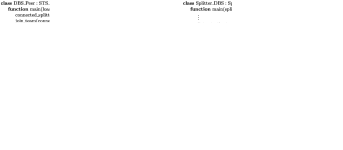
\includegraphics[width=\textwidth]{joining}
  \fig{1000}{10cm}{joining} \caption{Code related to team
    joining.\label{fig:joining}}
\end{figure*}

The new pseudo-code related to joining a team is describen in the
Fig.~\ref{fig:joining}.
\end{comment}

\begin{notex}
  See \href{https://github.com/P2PSP/simulator/blob/f0c73be1817e7d3b816cc61cd2c8e59b17f9a0e6/src/core/splitter_dbs.py#L296}{$\text{destination\_of\_chunk}[]$ in \texttt{peer\_dbs.py}}.
\end{notex}


\subsection{Buffering chunks}
%%% Local Variables:
%%% mode: latex
%%% TeX-master: "<none>"
%%% End:

\label{sec:buffering_chunks}

In order to hide the jitter generated by the physical network and the
protocol itself, peers need to store the received chunks in a buffer
during a period of time before playing them. A chunk with number $x$
is inserted in the position $(x \mathit{mod} 2B)$ of the buffer, where
$B$ is the maximum number of chunks that the buffer will store. In a
peer's life, $B$ is constant, but it is not compulsory that all peers
of the same team use the same $B$ value.

The buffer is implemented as a circular queue of $2B$ chunks, which is
filled up to only $B$ chunks in the buffering time (which is the main
part of the start-up time that the users experiment). Chunks with a
higher number (newer chunks) are inserted in the head of the
buffer. The chunk pointed by the tail of the buffer is sent to the
player (if there is a chunk in that cell of the buffer). This action
is carried out each time a new chunk is received.

Chunks can be lost.\footnote{Chunks are transmitted using a
  unrealiable communication, and therefore, network congestion can
  lose chunks.} A chunk is considered as lost when it is time to send
it to the player and the chunk has not been received.  In this
situation, for each lost chunk, the peer sends a $[\mathtt{request}
  \text{lost\_chunk\_number}]$ (that is the number of the next chunk
to be played) to the last neighbor served. When a peer $P_x$ receives
a $[\mathtt{request} \text{lost\_chunk\_number}]$ from $P_y$, $P_x$
adds $P_y$ to $\text{forward}[P_o]$, where $P_o$ is the origin peer of
the chunk stored in the position $lost\_chunk\_number$ of the buffer.

% As an alternative ...
\begin{comment}
origin peer of the next chunk stored in the
buffer. This peer has to characteristics: (1) it is not necessary a
neighbor peer, and (2) there is a high probability that this chunk has
been stored in the buffer ``for a long time'', so, if it is not a
neighbor, the link between it and the peer is working fairly well.
\end{comment}

\begin{notex}
  In the current implementation, the destination of the
  $[\mathtt{request} ...]$ message is the neighbor with the smaller
  chunk debt. This, a priori, has the drawback that this peer will
  always selected for relaying all the lost chunks because i will have
  a smaller debt as a consequence of the requests.
\end{notex}
  
In this situation, it is also possible that some peers can request
redundant paths between an origin peer and itself, and therefore, some
chunks could be received more than once. If this case, for each
duplicate chunk, a peer $P_i$ should send a $[\mathtt{prune}
  \text{duplicate\_chunk\_number}]$ message to those neighbors that
have sent to it the duplicate chunk. Neighbors receiving such message
from peer $P_i$ should remove the $P_i$ from $\text{forward}[P_o]$,
where $P_o$ is the origin peer of the duplicate chunk.

\begin{comment}
\begin{figure*}
  \fig{500}{5cm}{DBS_peer_buffering} \caption{Buffering of the
    chunks.\label{fig:DBS_peer_buffering}}
\end{figure*}
\end{comment}

The buffering time determines how much time the peers must wait before
start playing the chunks. Considering that chunks can be lost in
transit or delayed more than $B$ times of chunk, randomly, it is
difficult to determine, a priori the optimal buffering time. In the
current implementation, peers buffer a variable number of chunks that
depends on the order in which chunks are received. If $x_1$ is the
(number of the) first chunk received (the first chunk to be played),
the buffering time finishes when the chunk $x_1+B$ is
received.\footnote{Notice that all chunks with a number smaller than
  $x_1$ will be discarded, and that during the buffering time, it can
  happens that some chunks are not received on time. Therefore, it
  does not make sense to wait for $B$ chunks before stopping the
  buffering process.}

% Hablar de la relación entre B y el tamaño del team. Tal vez, cuando
% se presente la expresión de la latencia en función del grado de
% conectividad. En el caso extremo en que todos los peers se
% conectaran con todos, B >= N^*, el número máximo de peer en el team.

\begin{comment}
An heuristic that
works is the described in the Fig.~\ref{fig:DBS_peer_buffering}. As
can be seen, $\text{chunk\_to\_play}$ points to the first received
chunk, that not necessary is the received chunk with lower
index. After that, the
buffering finishes when a chunk with index $\text{chunk\_to\_play} +
\text{BUFFER\_SIZE}/2$ has been received.\footnote{This not means that
  $\text{BUFFER\_SIZE}/2$ chunks are available in the buffer.}
\end{comment}


\subsection{Chunk flooding}
\label{sec:chunk_flooding}
\begin{figure*}
  %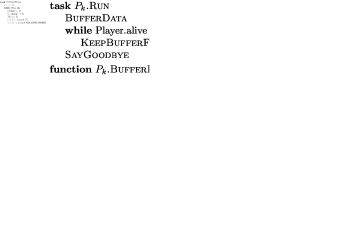
\includegraphics[width=0.75\textwidth]{chunk_generation_and_flooding}
  \fig{100}{3cm}{peer_chunk_flooding}
  \caption{Chunk flooding at peers.\label{fig:peer_chunk_flooding}}
\end{figure*}
When a peer $P_k$ receives a chunk from $P_i$, $P_k$ floods the
chunk to $T^k \setminus P_i$, using a prioritized round-robin
schema (see Fig.~\ref{fig:chunk_flooding}). Besides, if
it is a duplicate chunk, $P_k$ sends to $P_i$ a
$[\mathtt{NRFCF}~P_l]$ ($\mathtt{N}$ot $\mathtt{R}$elay
$\mathtt{F}$uture $\mathtt{C}$hunks $\mathtt{F}$rom) message, where
$P_l$ is the origin peer of the duplicate chunk. Thus, only
the first neighbor $P_i$ to send to $P_k$ a chunk
``originated'' at $P_l$ will do that in the future, at least
that $P_k$ revokes this routing information by sending a
$[\mathtt{RFCF}~P_l]$ ($\mathtt{R}$elay $\mathtt{F}$uture
$\mathtt{C}$hunks $\mathtt{F}$rom) to one or more (possibly the rest
of) peers of $T^k$.

As it has been said before, peers prioritize the flooding of the
chunks they relay by sending first the chunks to those neighbors that
are more supportive. To achieve that, every time $Pj_k$ sends a chunk
to $P_l$, $P_k$ runs $\mathtt{debt}[P_l] = \mathtt{debt}[P_l]+1$, and
$P_l$ runs $\mathtt{debt}[P_k] = \mathtt{debt}[P_k]-1$ (see
Fig.\ref{fig:}). Basically, these tables maintain a ``debt'' of chunks
between evey pair of neighbor peers. In ideal circunstances, debs
should be $0$. Debs are clipped to
$\pm\mathtt{debt}_{\text{max}}$. Obviously, a high supportivity means
a low debt, and viceversa.

\begin{comment}
In each round, peers check if a chunk have been received from the rest
of peers of the team (${\cal P}_k\in {\cal T}_j)$). If not, peers send
a $[\mathtt{propagate}~{\cal P}_i]$ to one or more (possibly
to the rest of) peers of the team, where ${\cal P}_i$ is the origin peer
of the missing chunk. At this point, the process continues as
described in Section~\ref{dbs:chunk_flooding}.
\end{comment}

\begin{comment}
For each ${\cal P}_k\in N({\cal P}_i)$, ${\cal P}_i$ checks if a chunk
has been received from ${\cal P}_k$. If ${\cal P}_i$ detects that
${\cal P}_k$ has not sent a chunk to it during $L$ consecutive rounds,
performs $N({\cal P}_i) = N({\cal P}_i)\setminus{\cal P}_k$, and stops
sending to ${\cal P}_k$ more chunks.
\end{comment}
\begin{comment}
computes a
``chunk-debt'', denoted by $d({\cal P}_k)$, that is incremented each
time a chunk is received from ${\cal P}_k$ and decremented each time a
chunk is sent to ${\cal P}_k$. If ${\cal P}_i$ verifies that $d({\cal
  P}_k)>D$ (the maximum debt), then ${\cal P}_i$ considers that ${\cal
  P}_k$ is unable to communicate with it, performs $N({\cal P}_i) =
N({\cal P}_i)\setminus{\cal P}_k$, and stops sending to ${\cal P}_k$
more chunks.
\end{comment}


%When peers receive chunks from their splitter, they must flood them to
%their neighbors until the chunks are broadcasted to the whole team
%(Fig.~\ref{fig:chunk_generation_and_flooding}). Lets suppose that
%${\cal P}_k$ receives a chunk. In the case the sender is its splitter,
%${\cal P}_k$ floods the chunk to $N({\cal P}_k)$. However, if the
%sender is a peer ${\cal P}_m\in N({\cal P}_k)$, ${\cal P}_k$ adds
%${\cal P}_m$ to $N({\cal P}_k)$ if ${\cal P}_m$ is a new neighbor, and
%forwards the chunk to the rest of its neighborhood ${\cal P}_n\in
%N({\cal P}_k)\setminus{\cal P}_m$ if ${\cal P}_k$ is in the shortest
%between ${\cal P}_n$ and the origin peer ${\cal P}_i$ of the relayed
%chunk. This will be true if ${\cal P}_k$ is the gateway of ${\cal
%  P}_n$ to go from ${\cal P}_n$ to ${\cal P}_i$. Therefore, a flooding
%with prunning based on shortest path routing is used.


\subsection{Routes discovery and topology optimization}
% Emacs, this is -*-latex-*-

% Routes Discovery and Topology Optimization

\label{sec:routes_discovery}

Chunks can be lost under bandwidth and buffering time constraints. A
chunk is lost when it is time to send it to the player, i.e. when it
is pointed by $p_p$, and the chunk has not been received. 
When a peer realizes that a chunk pointed by $p_p$ has been lost,
nothing can be done to recover it. Peers pre-fetch ``potentially
lost'' chunks at the buffer position $p_p+p_h$, where $p_h\geq 0$ is
the pre-feching horizon. Setting $p_h=0$, the pre-fetching is
disabled and only those chunks that really are lost will be
requested \leorem{no entiendo para que se piden}. 
On the contrary, the higher the $p_h$, the more aggressive
the pre-fetching is.  

For each (potentially) lost chunk with number
$\text{lost\_chunk\_number}$, peers send a
$[\mathtt{request}~\text{lost\_chunk\_number}]$ message to a random
peer of the team\leorem{solo uno? cuando se produce pruning?}. When a peer $P_i$ receives such message from 
$P_j$, $P_i$ adds $P_j$ to $\mathtt{forward}[P_k]$. $P_k$ is the
origin peer of the chunk stored in the position
$(\text{lost\_chunk\_number}~\mathit{mod}~2B)$ of $P_i$'s buffer in case this
chunks has been received. Otherwise, the request is ignored \leorem{y cómo se recupera?}. Notice
that, although request messages are very short, they are an overhead.

When request messages are used, redundant routes can be created and
therefore, some chunks could be received more than once. This is an overhead to be minimized. \leo{Upon the reception of the lost chunk, a peer send a pruning message to the other requested peers}. The receiver of the pruning message counts the number of times that a origin peer has been pruned, and when this counter is higher than a threshold $T$ (the maximum number of generated duplicates \leo{at requester's side}), the corresponding entry in the $\text{forward}[]$ table is deleted \leorem{Es por chunk o por origen?}.

Now, we can define more accurately the \gls{neighborhood-degree} (see
Sec.~\ref{sec:chunk_flooding}) as the number of different destination
peers for each possible origin that a peer forwards. For example, if a
peer $P_i$ forwards chunks from the origin $P_i$ to 10 neighbors, the
neighborhood degree of $P_i$ for the origin $P_i$ is 10, and if the
peer $P_i$ also forwards chunks from an origin $P_j$ to 5 neighbors,
the neighborhood degree of $P_i$ for the origin $P_j$ is 5\leorem{yo definiría dos tipos de grado de vecindad, el mio y el de reenvio}.

Considering the rules described before, the neighborhood degrees of
peers can decrease or increase to optimize the topology of the
overlay, by minimizing $\Delta t_b$. An increment in the degree for the origin of a requested
chunk $\text{lost\_chunk\_number}$ in $P_i$ is produced when $P_i$
recives a $[\mathtt{request}~\text{lost\_chunk\_number}]$ from a peer
that is not a neighbor, yet. On the contrary, a decrement in the
degree for the origin of a pruned chunk
$\text{duplicate\_chunk\_index}$ in $P_i$ is produced when $P_i$
receives a $[\mathtt{prune}~\text{duplicate\_chunk\_index}]$ from a
neighbor peer, for that origin. In fact, the continued use of the
requesting and pruning messages produce in a peer $P_i$ that the list
$\text{forward}[P_i]$ gets shorter (smaller \gls{neighborhood-degree})
and new entries in the table $\text{forward}[]$ are created.


%\subsection{Overlay topology optimization and the neighborhood degree}
%The neighborhood degree can also grow. When a chunk is lost, the peer
requests to receive the rest of chunks from the corresponding origin
peer to a random peer of the team. If duplicates are generated, prune
messages will remove the slower routes from that origin peer,
generating that the most reliable (and possiblely faster) route to
endure. When this happens, the requesting peer will be added to
$\mathtt{forward}[]$ (and therefore, sooner or later to
$\mathtt{pending}[]$) table of the requested peer, increasing its
neighborhood degree.


\subsection{Leaving a team}
\begin{figure*}
  %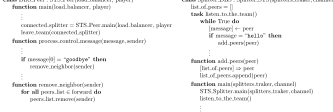
\includegraphics[width=0.55\textwidth]{leaving}
  \fig{300}{4cm}{leaving}
  \caption{Peer leaving.\label{fig:leaving}}
\end{figure*}
An outgoing peer $P^t_o$ (see Fig.~\ref{fig:leaving}) must to: (1) say
$[\mathtt{goodbye}]$ to $S^t$ and to $T^t_o$ (in this order), (2)
relay any pending (received but yet not sent) chunks, and (3) wait for
a $[\mathtt{goodbye}]$ from $S^t$, which performs $T^t = T^t \setminus
P^t_o$. In case of a timeout, $P^t_o$ resets the leaving procedure,
for a maximum number of times.

When a $P^t_k$ receives a $[\mathtt{goodbye}]$ from $P^t_o$, $P^t_k$
removes $P^t_o$ from its neighbors set, by running $T^t_k = T^t_k
\setminus P^t_o$.


\subsection{Free-riding control}
% Emacs, this is -*-latex-*-

% Free-riding Control at the Splitter

\label{sec:free_riding_control}

The splitter remembers which chunk, of a list of the last $B'$
transmitted chunks, was sent to each peer of the team. Notice that, in
order to remember the chunk that was sent to each peer in each round,
it must be hold that $B'\ge N$. \note{See
  \href{https://github.com/P2PSP/simulator/blob/f0c73be1817e7d3b816cc61cd2c8e59b17f9a0e6/src/core/splitter_dbs.py\#L296}{$\text{destination\_of\_chunk}[]$
    in \texttt{splitter\_dbs.py}}.}

Monitor peers (which are trusted peers) complain to their splitter
with a $[\mathtt{lost}~\text{lost\_chunk\_number}]$ for each lost
chunk. The splitter only considers these type of messages if they come
from a monitor.

%Notice that $L$ will
%tend to be proportional to the number $M$ of monitors, especially if
%those cases where $P_o$ is a gone peer that was unable to transmit the
%$[\mathtt{goodbye}]$ messages.

\begin{notex}
This last functionality has not been implemented, at least, as it has
been explained here. The forget() thread is controlled by a timer, not
by a counter of rounds.
\end{notex}

%Peers also control that at least one chunk is received from a neighbor
%in each round.\footnote{Peers recognize that a new round has started
%  when a new chunk is received from the splitter.} If happens that a
%peer $P_x$ does not receives a chunk from peer $P_y$ between $D^*$
%consecutive rounds, $P_x$ removes $P_y$ of its forwaring table.


%\subsection{Free-riding control at peers} % Neighborhood dynamics
%\label{dbs:frcp}
%Every time ${\cal P}^j_k$ sends a chunk to ${\cal P}^j_l$, ${\cal
P}^j_k$ runs $\mathtt{debt}[{\cal P}^j_l] = \mathtt{debt}[{\cal
P}^j_l]+1$, and ${\cal P}^j_l$ runs $\mathtt{debt}[{\cal P}^j_k]
= \mathtt{debt}[{\cal P}^j_k]-1$ (see Fig.\ref{fig}). Basically, these tables
maintain a ``debt'' of chunks between evey pair of neighbor
peers. If ${\cal P}^j_k$ realises that $\mathtt{debt}[{\cal
P}^j_l]>\mathtt{debt}_\text{max}$, then ${\cal P}^j_k$ removes ${\cal
P}^j_l$ from ${\cal T}^j_k$. Debts are clipped to $0$.

\begin{comment}
In each round, peers check if a chunk have been received from the rest
of peers of the team (${\cal P}_k\in {\cal T}_j)$). If not, peers send
a $[\mathtt{propagate}~{\cal P}_i]$ to one or more (possibly
to the rest of) peers of the team, where ${\cal P}_i$ is the origin peer
of the missing chunk. At this point, the process continues as
described in Section~\ref{dbs:chunk_flooding}.
\end{comment}

\begin{comment}
For each ${\cal P}_k\in N({\cal P}_i)$, ${\cal P}_i$ checks if a chunk
has been received from ${\cal P}_k$. If ${\cal P}_i$ detects that
${\cal P}_k$ has not sent a chunk to it during $L$ consecutive rounds,
performs $N({\cal P}_i) = N({\cal P}_i)\setminus{\cal P}_k$, and stops
sending to ${\cal P}_k$ more chunks.
\end{comment}
\begin{comment}
computes a
``chunk-debt'', denoted by $d({\cal P}_k)$, that is incremented each
time a chunk is received from ${\cal P}_k$ and decremented each time a
chunk is sent to ${\cal P}_k$. If ${\cal P}_i$ verifies that $d({\cal
  P}_k)>D$ (the maximum debt), then ${\cal P}_i$ considers that ${\cal
  P}_k$ is unable to communicate with it, performs $N({\cal P}_i) =
N({\cal P}_i)\setminus{\cal P}_k$, and stops sending to ${\cal P}_k$
more chunks.
\end{comment}


%\subsection{Congestion control}
%\label{dbs:congestion_control}
%P2PSP is a content-unaware push-based protocol. To avoid network
congestion while flooding, sending peers must perform some kind of
data flow-control. Moreover, to achieve aN ideal I/O ratio of $1$,
peers should send one chunk for every received one.

Congestion control in P2PSP is very simple: if a new chunk is
received, peers forward (using the flooding with prunning algorithm
described in Sec~\ref{dbs:chunk_generation_and_flooding}) each
received chunk to the next peer of their list of peers (following a
round-robin pattern).

%Peers do not understand the content, but it is
%known that in order to achieve a I/O ratio of 1, peers should send one
%chunk for every received one, on average. To acomplish this, a ${\cal
%  P}_i$ creates a FIFO queue of chunks for each $N({\cal P}_i)$, and,
%for each received chunk, ${\cal P}_i$ forwards a queued chunk from
%each of these queues.

\begin{comment}
A ${\cal P}_i$ forwards one or more chunks if and only if it has
received a chunk. For each received chunk $c_j$, ${\cal P}_i$: 1)
creates a list $l_{c_j}$ with the contents of $N'({\cal P}_i)$, and 2)
sends $c_j$ to $l_{c_j}[0]$ (the first element), and removes
$l_{c_j}[0]$. For each chunk reception, Step 2) is repeated for all
the previously created lists while they are not exhausted.

A solution is a forwarding algorithm based on the following
idea. Peers manage a list of chunks, where every item is a 2-tuple
($c_k$, $P_l$). The field $c_k$ represents the chunk that must be
flooded (if the node that has delivered the chunk is the splitter,
$c_k$ must be relayed towards all the neighbors, otherwise, $c_k$ must
be sent to all the neighbors except the peer that delivered $c_k$),
and the field $P_l$ the last neighbor to which $c_k$ was sent. For
every chunk received, a new tuple is appended to the list of chunks
and the rest of tuples are updated. The field $c_k$ remains constant
but $P_l$ is replaced by the next peer in the list of neighbors for
every received chunk.
\end{comment}


\begin{comment}
\subsubsection{Flooding order}
\label{dbs:flooding_order}
As an incentive mechanism~\cite{xu2006analysis}, peers relay received
chunks first to those peers that 
\end{comment}

%neighbors with lower chunk-debts.

\begin{comment}
\subsubsection{Team dynamics}
\label{dbs:team_dynamics}
${\cal P}_i$ adds to $N({\cal P}_i)$ those ${\cal P}_j$ that has sent
to ${\cal P}_i$ a chunk. If $N({\cal P}_i)>K$, periodically, ${\cal
  P}_i$ removes from $N({\cal P}_i)$ the peer with highest chunk-debt
and try to find in ${\cal T}_j\setminus N({\cal P}_i)$ a new peer using
$[\mathtt{hello}]$ messages.
\end{comment}

\begin{comment}
Peers use a buffer $b$ of chunks to hide the jitter generated by the
physical network and the broadcasting protocol. When a peer receives
$C_i$, it performs
\begin{equation}
  b[i~\text{mod}~B] = c_i,
\end{equation}
where ``mod'' represents the modulo operator and $B$ the buffer size
(in chunks). Basically, the buffer represents a sliding window that
moves over the stream synchronizely with the playing because the the
player consumes the chunks at the same chunk-rate the source produces
them.
\end{comment}

%%%%%%%%%%

\begin{comment}

\begin{itemize}

\item In the P2PSP, only monitor peers complains about lost
  chunks. This means that if a chunk that has been retransmitted by a
  peer is lost, it will be only retransmitted to all the peers of the
  team if the destination is a monitor peer and there is a unique
  monitor peer in the team. On the other hand, if the lost chunk was
  traveling from the splitter to a peer, all monitor peers will
  complain and this chunk will be retransmitted to the complete
  team. Therefore, only massively loss chunks will be retransmitted in
  the P2PSP. However, notice that a isolated missing chunk will
  produce negligible artifacts in the playback of one peer. In the
  Chain model, the lost of a chunk is handled between neighbour peers
  which means that all lost blocks should be, a priori, recovered.

\end{itemize}

\end{comment}



\begin{comment}
\subsubsection{Shortest path computation}
\label{dbs:chunk_routing}
\begin{figure}
  %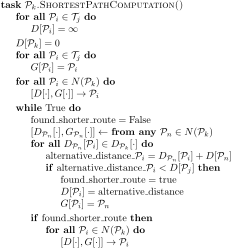
\includegraphics[width=0.35\textwidth]{shortest_path_computation}
  \fig{500}{4cm}{shortest_path_computation}
  \caption{Shortest path computation.\label{fig:shortest_path_computation}}
\end{figure}
The shortest path distances among peers are determined by a variation
of the Bellman-Ford Algorithm~\cite{Bertsekas1987data} (see
Fig.~\ref{fig:shortest_path_computation}), where the cost of the
``links'' between neighbor peers is $1$. Neighbor peers interchange
two vectors $D[\cdot]$ (distance-to-peer) and $G[\cdot]$
(gateway-to-peer) and compute the shortest distances and the (peer)
gateways to (reach) the rest of peers of its team ${\cal T}_j$.

This algorithm is free of routing loops and is not suceptible of the
well known count-to-infinity problem, and therefore always converges
for static teams. These problems do not appear because the routes are 

Each peer ${\cal P}_k$ sends
its vector of distances $D[\forall {\cal P}_i\in T^*({\cal P}_k)]$ and
gateways $G[\forall {\cal P}_i\in T^*({\cal P}_k)]$ to each
neighbor. When this information is received, peers check if shorter
routes can be found to the rest of peers of the reachable team, and if
so, send these vectors again.

The Bellman-Ford algorithm is susceptible of routing loops and the
count-to-infinite problem.


% Hace falta saber desde dónde viene el chunk original (origin peer) y que todos los peers dispongan de los vector-distances de los peers vecinos. Los vector-ditances deben tener tantas entradas como peers existen en el team. Por tanto, cada peer almacena un número de vector-distances igual a su grado de conectividad.


% Supposing that the weight of links between neighbors is 1.
% ¿Cómo sabe un peer que él es el último?
\end{comment}

\begin{comment}
\subsubsection{Generation of the routing tables}
Routing tables has as many entries as peers are in the team. The
routing table of a peer $P_i$ is a dictionary of pairs ($d(P_i, P_j)$,
$P_k$) indexed by the destination peer $P_j$ is a destination peer,
where $d(P_i, P_j)$ is the last measurement of the number of hops (in
peers) between $P_i$ and $P_j$, and $P_k\in N(P_i)$ is the 1-hop peer
that in the shortest-path between $P_i$ and $P_j$. Notice that if
$P_j==P_k$ then $d(P_i, P_j)==1$, which means that $P_i$ and $P_j$ are
directly ``connected''.

When a peer has updated its routing table, it is sent to their
neighbors pyggibacked on a \textsf{chunk} packet. When a peer receives
a routing table, it keeps a copy of it and updates its own routing
table with the new routing information using the Bellman-Ford
Algorithm~\cite{}. The peers have a copy of the routing table of its
neighbors to use it through the chunk routing process (see
Rule~\cite{the_routing_process}.
\end{comment}



\section{MCS (Multi-Channel Set)}
\label{sec:DBS}
DBS provides ALM for unicast (TCP/UDP) environments. The media is
received by a collection of
\emph{splitters} ${\cal S}=\{{\cal S}^0, \cdots, {\cal
  S}^{G-1}\}$ from a streaming server ${\cal O}$,
called \emph{source}, at a (usually variable) bit-rate which matches
the bit-rate of the media. Each ${\cal S}^i$ splits the
stream into a sequence of \emph{chunks}, and relay them to
different \emph{team} of up to $N$ \emph{peers}. We define the set of
teams as ${\cal T}=\{{\cal T}^0,\cdots,{\cal T}^{G-1}\}$ and the set
of peers per team $T^j=\{{\cal P}^j_0,\cdots,{\cal P}^j_{N-1}\}$.


%${\cal T}=\{{\cal T}_0,\cdots,{\cal T}_{G-1}\}$ \emph{teams} (one per
%  splitter) of up to $N$
%\emph{peers} $\{{\cal P}_0,\cdots,{\cal P}_{N-1}\}$, per team.


\subsection{Team definition and types of peers}
%%% Local Variables:
%%% mode: latex
%%% TeX-master: "<none>"
%%% End:

\label{sec:team_def}

A team is a set of one or more peers that share the same stream. By
definition, in a team of size one (the corresponding splitter is
considered out of the team if feeds), the only peer is known as a
\emph{monitor} peer, and in a team with more than one peer, at least
one of them must be a monitor peer. Monitors are instantiated by the
team administrator to monitorize different aspects of the
broadcasting, such as, the expected quality of the rendered video at
the peers or the expected average end-user latency.


\subsection{Feeding the team}
% Emacs, this is -*-latex-*-

% Feeding the Team

\label{sec:feeding_the_team}

The splitter divides the stream into chunks of constant length $C$,
and sends exclusively each chunk to a different
\gls{origin}\footnote{In the route that a chunk traces from the
  splitter to all peers of the team, the origin peer is the first one
  in this route i.e., the peer selected by the splitter for that
  chunk.}  peer, using a round-robin schema. Chunks are enumerated to
distinguish them, and this information is transmitted as a part of a chunk
header.

\begin{comment}
More details about the implementation
are available in Fig.~\ref{fig:chunk_generation}.

%$x$, conforming a message
%$c_x=[x,\text{chunk}]$, where
%$x=i \text{mod} \text{Splitter\_DBS.list\_of\_peers}.\text{length}()$.

\begin{figure*}
  %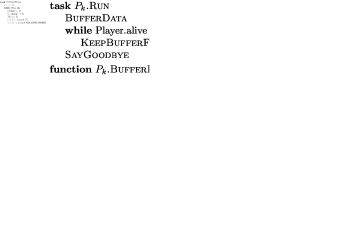
\includegraphics[width=0.75\textwidth]{chunk_generation_and_flooding}
  \fig{500}{5cm}{DBS_splitter_feed} \caption{Chunk
    generation at the splitter and their transmission to the
    team.\label{fig:chunk_generation}}
\end{figure*}
\end{comment}

A \gls{round} is defined as the process of transmitting $N$ different
chunks from the splitter to a team of $N\leq N^*$ peers (therefore,
all the peers of the team are origin of a different chunk, in each
round). For a team of size $N$, the average \gls{round-time} can be
estimated as
\begin{equation}
  t^{\mathrm{round}}=Nt^{\mathrm{chunk}},
\end{equation}
where $t^{\mathrm{chunk}}$ is the \gls{chunk-time}, defined as
\begin{equation}
  \label{eq:chunk_time}
  t^{\mathrm{chunk}}=\frac{l^{\mathrm{chunk}}}{R},
\end{equation}
where $l^{\mathrm{chunk}}$ is the length of the chunks (all the chunks are
split with the same length) and $R$ is the average transmission
bit-rate, that should match the average bit-rate of the stream in
order to achieve a seamsless playing.

\begin{comment}
The round-time is defined by:
\begin{equation}
  \cal{r} = \cal{c}N.
  \label{eq:round_time}
\end{equation}
For example, if we use only one team of $N=256$ peers, a chunk size
$C=1024$~bytes, and a video of $1$~Mb/s, the round time is
\begin{displaymath}
  \cal{r} = \frac{1024\frac{\text{bytes}}{\text{chunk}}\times
    8\frac{\text{bits}}{\text{byte}}}{10^6\frac{\text{bits}}{\text{second}}}\times
  256 \approx 2.1~\text{seconds}.
\end{displaymath}
\end{comment}


\subsection{Joining a team}
% Emacs, this is -*-latex-*-

% Joining the Team

\label{sec:joining}

After connecting with a splitter, incoming peers request (using a
reliable communication) to the splitter the current set of peers in
the team. To minimize the joining time, the peer sends a
$[\mathtt{hello}]$ message to each other peer of the team, in parallel
with the reception of the set. When a peer of the team receives a
$[\mathtt{hello}]$, it adds the sender of the message to a
\emph{table}\footnote{A structure which implements a random access
  efficiently.} of peers called $\mathtt{forward}[]$ \note{(see
  \href{https://github.com/P2PSP/simulator/blob/f0c73be1817e7d3b816cc61cd2c8e59b17f9a0e6/src/core/peer_dbs.py\#L491}{$\text{forward[]}$
    in \texttt{peer.py}})}. If a peer $P_i$ has an entry
$\mathtt{forward}[P_j]=P_k$, then each chunk received by $P_i$ and
originated at $P_j$ will be forwarded to $P_k$. When an incoming peer
$P_i$ has received the set of peers, its forwarding table has been
initialized to $\mathtt{forward}[P_i]=\{\text{team}\setminus
P_i\}$. Notice that, as long as the forwarding table contains this
information, all chunks received from the splitter will be forwarded
to the rest of the team, directly (in one protocol hop). So, in
absence of communication constraints, the team will be organized as a
full-connected overlay (see Fig.~\ref{fig:full_mesh}).

%), initializes
%the table $\mathrm{debt}[]$ (which stores the chunk debts between
%neighbor peers), and (3) sets the variable $\mathrm{neighbor}$ with an
%index to $\mathrm{forward}[]$ (see
%Sec.~\ref{sec:chunk_DBS_processing}).

The splitter, in an infinite loop: (1) listens to the incoming peers,
(2) sends to them the set of peers of the team, and (3) includes the
incoming peer to the set. Notice that only those peers that are in
the set of peers of the splitter are considered to be in the team
served by such splitter.

\begin{comment}
\begin{figure*}
  %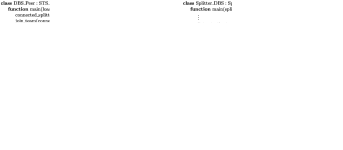
\includegraphics[width=\textwidth]{joining}
  \fig{1000}{10cm}{joining} \caption{Code related to team
    joining.\label{fig:joining}}
\end{figure*}

The new pseudo-code related to joining a team is describen in the
Fig.~\ref{fig:joining}.
\end{comment}

\begin{notex}
  See \href{https://github.com/P2PSP/simulator/blob/f0c73be1817e7d3b816cc61cd2c8e59b17f9a0e6/src/core/splitter_dbs.py#L296}{$\text{destination\_of\_chunk}[]$ in \texttt{peer\_dbs.py}}.
\end{notex}


\subsection{Buffering chunks}
%%% Local Variables:
%%% mode: latex
%%% TeX-master: "<none>"
%%% End:

\label{sec:buffering_chunks}

In order to hide the jitter generated by the physical network and the
protocol itself, peers need to store the received chunks in a buffer
during a period of time before playing them. A chunk with number $x$
is inserted in the position $(x \mathit{mod} 2B)$ of the buffer, where
$B$ is the maximum number of chunks that the buffer will store. In a
peer's life, $B$ is constant, but it is not compulsory that all peers
of the same team use the same $B$ value.

The buffer is implemented as a circular queue of $2B$ chunks, which is
filled up to only $B$ chunks in the buffering time (which is the main
part of the start-up time that the users experiment). Chunks with a
higher number (newer chunks) are inserted in the head of the
buffer. The chunk pointed by the tail of the buffer is sent to the
player (if there is a chunk in that cell of the buffer). This action
is carried out each time a new chunk is received.

Chunks can be lost.\footnote{Chunks are transmitted using a
  unrealiable communication, and therefore, network congestion can
  lose chunks.} A chunk is considered as lost when it is time to send
it to the player and the chunk has not been received.  In this
situation, for each lost chunk, the peer sends a $[\mathtt{request}
  \text{lost\_chunk\_number}]$ (that is the number of the next chunk
to be played) to the last neighbor served. When a peer $P_x$ receives
a $[\mathtt{request} \text{lost\_chunk\_number}]$ from $P_y$, $P_x$
adds $P_y$ to $\text{forward}[P_o]$, where $P_o$ is the origin peer of
the chunk stored in the position $lost\_chunk\_number$ of the buffer.

% As an alternative ...
\begin{comment}
origin peer of the next chunk stored in the
buffer. This peer has to characteristics: (1) it is not necessary a
neighbor peer, and (2) there is a high probability that this chunk has
been stored in the buffer ``for a long time'', so, if it is not a
neighbor, the link between it and the peer is working fairly well.
\end{comment}

\begin{notex}
  In the current implementation, the destination of the
  $[\mathtt{request} ...]$ message is the neighbor with the smaller
  chunk debt. This, a priori, has the drawback that this peer will
  always selected for relaying all the lost chunks because i will have
  a smaller debt as a consequence of the requests.
\end{notex}
  
In this situation, it is also possible that some peers can request
redundant paths between an origin peer and itself, and therefore, some
chunks could be received more than once. If this case, for each
duplicate chunk, a peer $P_i$ should send a $[\mathtt{prune}
  \text{duplicate\_chunk\_number}]$ message to those neighbors that
have sent to it the duplicate chunk. Neighbors receiving such message
from peer $P_i$ should remove the $P_i$ from $\text{forward}[P_o]$,
where $P_o$ is the origin peer of the duplicate chunk.

\begin{comment}
\begin{figure*}
  \fig{500}{5cm}{DBS_peer_buffering} \caption{Buffering of the
    chunks.\label{fig:DBS_peer_buffering}}
\end{figure*}
\end{comment}

The buffering time determines how much time the peers must wait before
start playing the chunks. Considering that chunks can be lost in
transit or delayed more than $B$ times of chunk, randomly, it is
difficult to determine, a priori the optimal buffering time. In the
current implementation, peers buffer a variable number of chunks that
depends on the order in which chunks are received. If $x_1$ is the
(number of the) first chunk received (the first chunk to be played),
the buffering time finishes when the chunk $x_1+B$ is
received.\footnote{Notice that all chunks with a number smaller than
  $x_1$ will be discarded, and that during the buffering time, it can
  happens that some chunks are not received on time. Therefore, it
  does not make sense to wait for $B$ chunks before stopping the
  buffering process.}

% Hablar de la relación entre B y el tamaño del team. Tal vez, cuando
% se presente la expresión de la latencia en función del grado de
% conectividad. En el caso extremo en que todos los peers se
% conectaran con todos, B >= N^*, el número máximo de peer en el team.

\begin{comment}
An heuristic that
works is the described in the Fig.~\ref{fig:DBS_peer_buffering}. As
can be seen, $\text{chunk\_to\_play}$ points to the first received
chunk, that not necessary is the received chunk with lower
index. After that, the
buffering finishes when a chunk with index $\text{chunk\_to\_play} +
\text{BUFFER\_SIZE}/2$ has been received.\footnote{This not means that
  $\text{BUFFER\_SIZE}/2$ chunks are available in the buffer.}
\end{comment}


\subsection{Chunk flooding}
\label{sec:chunk_flooding}
\begin{figure*}
  %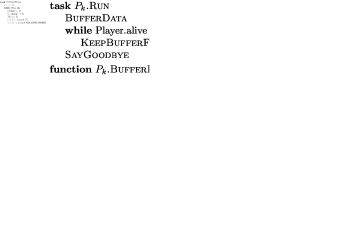
\includegraphics[width=0.75\textwidth]{chunk_generation_and_flooding}
  \fig{100}{3cm}{peer_chunk_flooding}
  \caption{Chunk flooding at peers.\label{fig:peer_chunk_flooding}}
\end{figure*}
When a peer $P_k$ receives a chunk from $P_i$, $P_k$ floods the
chunk to $T^k \setminus P_i$, using a prioritized round-robin
schema (see Fig.~\ref{fig:chunk_flooding}). Besides, if
it is a duplicate chunk, $P_k$ sends to $P_i$ a
$[\mathtt{NRFCF}~P_l]$ ($\mathtt{N}$ot $\mathtt{R}$elay
$\mathtt{F}$uture $\mathtt{C}$hunks $\mathtt{F}$rom) message, where
$P_l$ is the origin peer of the duplicate chunk. Thus, only
the first neighbor $P_i$ to send to $P_k$ a chunk
``originated'' at $P_l$ will do that in the future, at least
that $P_k$ revokes this routing information by sending a
$[\mathtt{RFCF}~P_l]$ ($\mathtt{R}$elay $\mathtt{F}$uture
$\mathtt{C}$hunks $\mathtt{F}$rom) to one or more (possibly the rest
of) peers of $T^k$.

As it has been said before, peers prioritize the flooding of the
chunks they relay by sending first the chunks to those neighbors that
are more supportive. To achieve that, every time $Pj_k$ sends a chunk
to $P_l$, $P_k$ runs $\mathtt{debt}[P_l] = \mathtt{debt}[P_l]+1$, and
$P_l$ runs $\mathtt{debt}[P_k] = \mathtt{debt}[P_k]-1$ (see
Fig.\ref{fig:}). Basically, these tables maintain a ``debt'' of chunks
between evey pair of neighbor peers. In ideal circunstances, debs
should be $0$. Debs are clipped to
$\pm\mathtt{debt}_{\text{max}}$. Obviously, a high supportivity means
a low debt, and viceversa.

\begin{comment}
In each round, peers check if a chunk have been received from the rest
of peers of the team (${\cal P}_k\in {\cal T}_j)$). If not, peers send
a $[\mathtt{propagate}~{\cal P}_i]$ to one or more (possibly
to the rest of) peers of the team, where ${\cal P}_i$ is the origin peer
of the missing chunk. At this point, the process continues as
described in Section~\ref{dbs:chunk_flooding}.
\end{comment}

\begin{comment}
For each ${\cal P}_k\in N({\cal P}_i)$, ${\cal P}_i$ checks if a chunk
has been received from ${\cal P}_k$. If ${\cal P}_i$ detects that
${\cal P}_k$ has not sent a chunk to it during $L$ consecutive rounds,
performs $N({\cal P}_i) = N({\cal P}_i)\setminus{\cal P}_k$, and stops
sending to ${\cal P}_k$ more chunks.
\end{comment}
\begin{comment}
computes a
``chunk-debt'', denoted by $d({\cal P}_k)$, that is incremented each
time a chunk is received from ${\cal P}_k$ and decremented each time a
chunk is sent to ${\cal P}_k$. If ${\cal P}_i$ verifies that $d({\cal
  P}_k)>D$ (the maximum debt), then ${\cal P}_i$ considers that ${\cal
  P}_k$ is unable to communicate with it, performs $N({\cal P}_i) =
N({\cal P}_i)\setminus{\cal P}_k$, and stops sending to ${\cal P}_k$
more chunks.
\end{comment}


%When peers receive chunks from their splitter, they must flood them to
%their neighbors until the chunks are broadcasted to the whole team
%(Fig.~\ref{fig:chunk_generation_and_flooding}). Lets suppose that
%${\cal P}_k$ receives a chunk. In the case the sender is its splitter,
%${\cal P}_k$ floods the chunk to $N({\cal P}_k)$. However, if the
%sender is a peer ${\cal P}_m\in N({\cal P}_k)$, ${\cal P}_k$ adds
%${\cal P}_m$ to $N({\cal P}_k)$ if ${\cal P}_m$ is a new neighbor, and
%forwards the chunk to the rest of its neighborhood ${\cal P}_n\in
%N({\cal P}_k)\setminus{\cal P}_m$ if ${\cal P}_k$ is in the shortest
%between ${\cal P}_n$ and the origin peer ${\cal P}_i$ of the relayed
%chunk. This will be true if ${\cal P}_k$ is the gateway of ${\cal
%  P}_n$ to go from ${\cal P}_n$ to ${\cal P}_i$. Therefore, a flooding
%with prunning based on shortest path routing is used.


\subsection{Routes discovery and topology optimization}
% Emacs, this is -*-latex-*-

% Routes Discovery and Topology Optimization

\label{sec:routes_discovery}

Chunks can be lost under bandwidth and buffering time constraints. A
chunk is lost when it is time to send it to the player, i.e. when it
is pointed by $p_p$, and the chunk has not been received. 
When a peer realizes that a chunk pointed by $p_p$ has been lost,
nothing can be done to recover it. Peers pre-fetch ``potentially
lost'' chunks at the buffer position $p_p+p_h$, where $p_h\geq 0$ is
the pre-feching horizon. Setting $p_h=0$, the pre-fetching is
disabled and only those chunks that really are lost will be
requested \leorem{no entiendo para que se piden}. 
On the contrary, the higher the $p_h$, the more aggressive
the pre-fetching is.  

For each (potentially) lost chunk with number
$\text{lost\_chunk\_number}$, peers send a
$[\mathtt{request}~\text{lost\_chunk\_number}]$ message to a random
peer of the team\leorem{solo uno? cuando se produce pruning?}. When a peer $P_i$ receives such message from 
$P_j$, $P_i$ adds $P_j$ to $\mathtt{forward}[P_k]$. $P_k$ is the
origin peer of the chunk stored in the position
$(\text{lost\_chunk\_number}~\mathit{mod}~2B)$ of $P_i$'s buffer in case this
chunks has been received. Otherwise, the request is ignored \leorem{y cómo se recupera?}. Notice
that, although request messages are very short, they are an overhead.

When request messages are used, redundant routes can be created and
therefore, some chunks could be received more than once. This is an overhead to be minimized. \leo{Upon the reception of the lost chunk, a peer send a pruning message to the other requested peers}. The receiver of the pruning message counts the number of times that a origin peer has been pruned, and when this counter is higher than a threshold $T$ (the maximum number of generated duplicates \leo{at requester's side}), the corresponding entry in the $\text{forward}[]$ table is deleted \leorem{Es por chunk o por origen?}.

Now, we can define more accurately the \gls{neighborhood-degree} (see
Sec.~\ref{sec:chunk_flooding}) as the number of different destination
peers for each possible origin that a peer forwards. For example, if a
peer $P_i$ forwards chunks from the origin $P_i$ to 10 neighbors, the
neighborhood degree of $P_i$ for the origin $P_i$ is 10, and if the
peer $P_i$ also forwards chunks from an origin $P_j$ to 5 neighbors,
the neighborhood degree of $P_i$ for the origin $P_j$ is 5\leorem{yo definiría dos tipos de grado de vecindad, el mio y el de reenvio}.

Considering the rules described before, the neighborhood degrees of
peers can decrease or increase to optimize the topology of the
overlay, by minimizing $\Delta t_b$. An increment in the degree for the origin of a requested
chunk $\text{lost\_chunk\_number}$ in $P_i$ is produced when $P_i$
recives a $[\mathtt{request}~\text{lost\_chunk\_number}]$ from a peer
that is not a neighbor, yet. On the contrary, a decrement in the
degree for the origin of a pruned chunk
$\text{duplicate\_chunk\_index}$ in $P_i$ is produced when $P_i$
receives a $[\mathtt{prune}~\text{duplicate\_chunk\_index}]$ from a
neighbor peer, for that origin. In fact, the continued use of the
requesting and pruning messages produce in a peer $P_i$ that the list
$\text{forward}[P_i]$ gets shorter (smaller \gls{neighborhood-degree})
and new entries in the table $\text{forward}[]$ are created.


%\subsection{Overlay topology optimization and the neighborhood degree}
%The neighborhood degree can also grow. When a chunk is lost, the peer
requests to receive the rest of chunks from the corresponding origin
peer to a random peer of the team. If duplicates are generated, prune
messages will remove the slower routes from that origin peer,
generating that the most reliable (and possiblely faster) route to
endure. When this happens, the requesting peer will be added to
$\mathtt{forward}[]$ (and therefore, sooner or later to
$\mathtt{pending}[]$) table of the requested peer, increasing its
neighborhood degree.


\subsection{Leaving a team}
\begin{figure*}
  %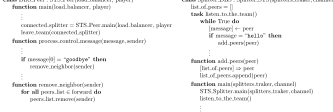
\includegraphics[width=0.55\textwidth]{leaving}
  \fig{300}{4cm}{leaving}
  \caption{Peer leaving.\label{fig:leaving}}
\end{figure*}
An outgoing peer $P^t_o$ (see Fig.~\ref{fig:leaving}) must to: (1) say
$[\mathtt{goodbye}]$ to $S^t$ and to $T^t_o$ (in this order), (2)
relay any pending (received but yet not sent) chunks, and (3) wait for
a $[\mathtt{goodbye}]$ from $S^t$, which performs $T^t = T^t \setminus
P^t_o$. In case of a timeout, $P^t_o$ resets the leaving procedure,
for a maximum number of times.

When a $P^t_k$ receives a $[\mathtt{goodbye}]$ from $P^t_o$, $P^t_k$
removes $P^t_o$ from its neighbors set, by running $T^t_k = T^t_k
\setminus P^t_o$.


\subsection{Free-riding control}
% Emacs, this is -*-latex-*-

% Free-riding Control at the Splitter

\label{sec:free_riding_control}

The splitter remembers which chunk, of a list of the last $B'$
transmitted chunks, was sent to each peer of the team. Notice that, in
order to remember the chunk that was sent to each peer in each round,
it must be hold that $B'\ge N$. \note{See
  \href{https://github.com/P2PSP/simulator/blob/f0c73be1817e7d3b816cc61cd2c8e59b17f9a0e6/src/core/splitter_dbs.py\#L296}{$\text{destination\_of\_chunk}[]$
    in \texttt{splitter\_dbs.py}}.}

Monitor peers (which are trusted peers) complain to their splitter
with a $[\mathtt{lost}~\text{lost\_chunk\_number}]$ for each lost
chunk. The splitter only considers these type of messages if they come
from a monitor.

%Notice that $L$ will
%tend to be proportional to the number $M$ of monitors, especially if
%those cases where $P_o$ is a gone peer that was unable to transmit the
%$[\mathtt{goodbye}]$ messages.

\begin{notex}
This last functionality has not been implemented, at least, as it has
been explained here. The forget() thread is controlled by a timer, not
by a counter of rounds.
\end{notex}

%Peers also control that at least one chunk is received from a neighbor
%in each round.\footnote{Peers recognize that a new round has started
%  when a new chunk is received from the splitter.} If happens that a
%peer $P_x$ does not receives a chunk from peer $P_y$ between $D^*$
%consecutive rounds, $P_x$ removes $P_y$ of its forwaring table.


%\subsection{Free-riding control at peers} % Neighborhood dynamics
%\label{dbs:frcp}
%Every time ${\cal P}^j_k$ sends a chunk to ${\cal P}^j_l$, ${\cal
P}^j_k$ runs $\mathtt{debt}[{\cal P}^j_l] = \mathtt{debt}[{\cal
P}^j_l]+1$, and ${\cal P}^j_l$ runs $\mathtt{debt}[{\cal P}^j_k]
= \mathtt{debt}[{\cal P}^j_k]-1$ (see Fig.\ref{fig}). Basically, these tables
maintain a ``debt'' of chunks between evey pair of neighbor
peers. If ${\cal P}^j_k$ realises that $\mathtt{debt}[{\cal
P}^j_l]>\mathtt{debt}_\text{max}$, then ${\cal P}^j_k$ removes ${\cal
P}^j_l$ from ${\cal T}^j_k$. Debts are clipped to $0$.

\begin{comment}
In each round, peers check if a chunk have been received from the rest
of peers of the team (${\cal P}_k\in {\cal T}_j)$). If not, peers send
a $[\mathtt{propagate}~{\cal P}_i]$ to one or more (possibly
to the rest of) peers of the team, where ${\cal P}_i$ is the origin peer
of the missing chunk. At this point, the process continues as
described in Section~\ref{dbs:chunk_flooding}.
\end{comment}

\begin{comment}
For each ${\cal P}_k\in N({\cal P}_i)$, ${\cal P}_i$ checks if a chunk
has been received from ${\cal P}_k$. If ${\cal P}_i$ detects that
${\cal P}_k$ has not sent a chunk to it during $L$ consecutive rounds,
performs $N({\cal P}_i) = N({\cal P}_i)\setminus{\cal P}_k$, and stops
sending to ${\cal P}_k$ more chunks.
\end{comment}
\begin{comment}
computes a
``chunk-debt'', denoted by $d({\cal P}_k)$, that is incremented each
time a chunk is received from ${\cal P}_k$ and decremented each time a
chunk is sent to ${\cal P}_k$. If ${\cal P}_i$ verifies that $d({\cal
  P}_k)>D$ (the maximum debt), then ${\cal P}_i$ considers that ${\cal
  P}_k$ is unable to communicate with it, performs $N({\cal P}_i) =
N({\cal P}_i)\setminus{\cal P}_k$, and stops sending to ${\cal P}_k$
more chunks.
\end{comment}


%\subsection{Congestion control}
%\label{dbs:congestion_control}
%P2PSP is a content-unaware push-based protocol. To avoid network
congestion while flooding, sending peers must perform some kind of
data flow-control. Moreover, to achieve aN ideal I/O ratio of $1$,
peers should send one chunk for every received one.

Congestion control in P2PSP is very simple: if a new chunk is
received, peers forward (using the flooding with prunning algorithm
described in Sec~\ref{dbs:chunk_generation_and_flooding}) each
received chunk to the next peer of their list of peers (following a
round-robin pattern).

%Peers do not understand the content, but it is
%known that in order to achieve a I/O ratio of 1, peers should send one
%chunk for every received one, on average. To acomplish this, a ${\cal
%  P}_i$ creates a FIFO queue of chunks for each $N({\cal P}_i)$, and,
%for each received chunk, ${\cal P}_i$ forwards a queued chunk from
%each of these queues.

\begin{comment}
A ${\cal P}_i$ forwards one or more chunks if and only if it has
received a chunk. For each received chunk $c_j$, ${\cal P}_i$: 1)
creates a list $l_{c_j}$ with the contents of $N'({\cal P}_i)$, and 2)
sends $c_j$ to $l_{c_j}[0]$ (the first element), and removes
$l_{c_j}[0]$. For each chunk reception, Step 2) is repeated for all
the previously created lists while they are not exhausted.

A solution is a forwarding algorithm based on the following
idea. Peers manage a list of chunks, where every item is a 2-tuple
($c_k$, $P_l$). The field $c_k$ represents the chunk that must be
flooded (if the node that has delivered the chunk is the splitter,
$c_k$ must be relayed towards all the neighbors, otherwise, $c_k$ must
be sent to all the neighbors except the peer that delivered $c_k$),
and the field $P_l$ the last neighbor to which $c_k$ was sent. For
every chunk received, a new tuple is appended to the list of chunks
and the rest of tuples are updated. The field $c_k$ remains constant
but $P_l$ is replaced by the next peer in the list of neighbors for
every received chunk.
\end{comment}


\begin{comment}
\subsubsection{Flooding order}
\label{dbs:flooding_order}
As an incentive mechanism~\cite{xu2006analysis}, peers relay received
chunks first to those peers that 
\end{comment}

%neighbors with lower chunk-debts.

\begin{comment}
\subsubsection{Team dynamics}
\label{dbs:team_dynamics}
${\cal P}_i$ adds to $N({\cal P}_i)$ those ${\cal P}_j$ that has sent
to ${\cal P}_i$ a chunk. If $N({\cal P}_i)>K$, periodically, ${\cal
  P}_i$ removes from $N({\cal P}_i)$ the peer with highest chunk-debt
and try to find in ${\cal T}_j\setminus N({\cal P}_i)$ a new peer using
$[\mathtt{hello}]$ messages.
\end{comment}

\begin{comment}
Peers use a buffer $b$ of chunks to hide the jitter generated by the
physical network and the broadcasting protocol. When a peer receives
$C_i$, it performs
\begin{equation}
  b[i~\text{mod}~B] = c_i,
\end{equation}
where ``mod'' represents the modulo operator and $B$ the buffer size
(in chunks). Basically, the buffer represents a sliding window that
moves over the stream synchronizely with the playing because the the
player consumes the chunks at the same chunk-rate the source produces
them.
\end{comment}

%%%%%%%%%%

\begin{comment}

\begin{itemize}

\item In the P2PSP, only monitor peers complains about lost
  chunks. This means that if a chunk that has been retransmitted by a
  peer is lost, it will be only retransmitted to all the peers of the
  team if the destination is a monitor peer and there is a unique
  monitor peer in the team. On the other hand, if the lost chunk was
  traveling from the splitter to a peer, all monitor peers will
  complain and this chunk will be retransmitted to the complete
  team. Therefore, only massively loss chunks will be retransmitted in
  the P2PSP. However, notice that a isolated missing chunk will
  produce negligible artifacts in the playback of one peer. In the
  Chain model, the lost of a chunk is handled between neighbour peers
  which means that all lost blocks should be, a priori, recovered.

\end{itemize}

\end{comment}



\begin{comment}
\subsubsection{Shortest path computation}
\label{dbs:chunk_routing}
\begin{figure}
  %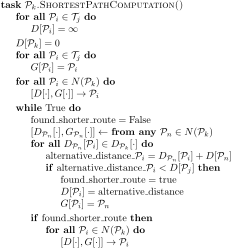
\includegraphics[width=0.35\textwidth]{shortest_path_computation}
  \fig{500}{4cm}{shortest_path_computation}
  \caption{Shortest path computation.\label{fig:shortest_path_computation}}
\end{figure}
The shortest path distances among peers are determined by a variation
of the Bellman-Ford Algorithm~\cite{Bertsekas1987data} (see
Fig.~\ref{fig:shortest_path_computation}), where the cost of the
``links'' between neighbor peers is $1$. Neighbor peers interchange
two vectors $D[\cdot]$ (distance-to-peer) and $G[\cdot]$
(gateway-to-peer) and compute the shortest distances and the (peer)
gateways to (reach) the rest of peers of its team ${\cal T}_j$.

This algorithm is free of routing loops and is not suceptible of the
well known count-to-infinity problem, and therefore always converges
for static teams. These problems do not appear because the routes are 

Each peer ${\cal P}_k$ sends
its vector of distances $D[\forall {\cal P}_i\in T^*({\cal P}_k)]$ and
gateways $G[\forall {\cal P}_i\in T^*({\cal P}_k)]$ to each
neighbor. When this information is received, peers check if shorter
routes can be found to the rest of peers of the reachable team, and if
so, send these vectors again.

The Bellman-Ford algorithm is susceptible of routing loops and the
count-to-infinite problem.


% Hace falta saber desde dónde viene el chunk original (origin peer) y que todos los peers dispongan de los vector-distances de los peers vecinos. Los vector-ditances deben tener tantas entradas como peers existen en el team. Por tanto, cada peer almacena un número de vector-distances igual a su grado de conectividad.


% Supposing that the weight of links between neighbors is 1.
% ¿Cómo sabe un peer que él es el último?
\end{comment}

\begin{comment}
\subsubsection{Generation of the routing tables}
Routing tables has as many entries as peers are in the team. The
routing table of a peer $P_i$ is a dictionary of pairs ($d(P_i, P_j)$,
$P_k$) indexed by the destination peer $P_j$ is a destination peer,
where $d(P_i, P_j)$ is the last measurement of the number of hops (in
peers) between $P_i$ and $P_j$, and $P_k\in N(P_i)$ is the 1-hop peer
that in the shortest-path between $P_i$ and $P_j$. Notice that if
$P_j==P_k$ then $d(P_i, P_j)==1$, which means that $P_i$ and $P_j$ are
directly ``connected''.

When a peer has updated its routing table, it is sent to their
neighbors pyggibacked on a \textsf{chunk} packet. When a peer receives
a routing table, it keeps a copy of it and updates its own routing
table with the new routing information using the Bellman-Ford
Algorithm~\cite{}. The peers have a copy of the routing table of its
neighbors to use it through the chunk routing process (see
Rule~\cite{the_routing_process}.
\end{comment}



\section{NTS (NAT Traversal Set)}
\label{sec:DBS}
DBS provides ALM for unicast (TCP/UDP) environments. The media is
received by a collection of
\emph{splitters} ${\cal S}=\{{\cal S}^0, \cdots, {\cal
  S}^{G-1}\}$ from a streaming server ${\cal O}$,
called \emph{source}, at a (usually variable) bit-rate which matches
the bit-rate of the media. Each ${\cal S}^i$ splits the
stream into a sequence of \emph{chunks}, and relay them to
different \emph{team} of up to $N$ \emph{peers}. We define the set of
teams as ${\cal T}=\{{\cal T}^0,\cdots,{\cal T}^{G-1}\}$ and the set
of peers per team $T^j=\{{\cal P}^j_0,\cdots,{\cal P}^j_{N-1}\}$.


%${\cal T}=\{{\cal T}_0,\cdots,{\cal T}_{G-1}\}$ \emph{teams} (one per
%  splitter) of up to $N$
%\emph{peers} $\{{\cal P}_0,\cdots,{\cal P}_{N-1}\}$, per team.


\subsection{Team definition and types of peers}
%%% Local Variables:
%%% mode: latex
%%% TeX-master: "<none>"
%%% End:

\label{sec:team_def}

A team is a set of one or more peers that share the same stream. By
definition, in a team of size one (the corresponding splitter is
considered out of the team if feeds), the only peer is known as a
\emph{monitor} peer, and in a team with more than one peer, at least
one of them must be a monitor peer. Monitors are instantiated by the
team administrator to monitorize different aspects of the
broadcasting, such as, the expected quality of the rendered video at
the peers or the expected average end-user latency.


\subsection{Feeding the team}
% Emacs, this is -*-latex-*-

% Feeding the Team

\label{sec:feeding_the_team}

The splitter divides the stream into chunks of constant length $C$,
and sends exclusively each chunk to a different
\gls{origin}\footnote{In the route that a chunk traces from the
  splitter to all peers of the team, the origin peer is the first one
  in this route i.e., the peer selected by the splitter for that
  chunk.}  peer, using a round-robin schema. Chunks are enumerated to
distinguish them, and this information is transmitted as a part of a chunk
header.

\begin{comment}
More details about the implementation
are available in Fig.~\ref{fig:chunk_generation}.

%$x$, conforming a message
%$c_x=[x,\text{chunk}]$, where
%$x=i \text{mod} \text{Splitter\_DBS.list\_of\_peers}.\text{length}()$.

\begin{figure*}
  %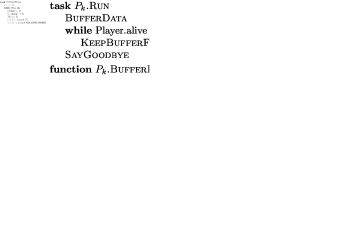
\includegraphics[width=0.75\textwidth]{chunk_generation_and_flooding}
  \fig{500}{5cm}{DBS_splitter_feed} \caption{Chunk
    generation at the splitter and their transmission to the
    team.\label{fig:chunk_generation}}
\end{figure*}
\end{comment}

A \gls{round} is defined as the process of transmitting $N$ different
chunks from the splitter to a team of $N\leq N^*$ peers (therefore,
all the peers of the team are origin of a different chunk, in each
round). For a team of size $N$, the average \gls{round-time} can be
estimated as
\begin{equation}
  t^{\mathrm{round}}=Nt^{\mathrm{chunk}},
\end{equation}
where $t^{\mathrm{chunk}}$ is the \gls{chunk-time}, defined as
\begin{equation}
  \label{eq:chunk_time}
  t^{\mathrm{chunk}}=\frac{l^{\mathrm{chunk}}}{R},
\end{equation}
where $l^{\mathrm{chunk}}$ is the length of the chunks (all the chunks are
split with the same length) and $R$ is the average transmission
bit-rate, that should match the average bit-rate of the stream in
order to achieve a seamsless playing.

\begin{comment}
The round-time is defined by:
\begin{equation}
  \cal{r} = \cal{c}N.
  \label{eq:round_time}
\end{equation}
For example, if we use only one team of $N=256$ peers, a chunk size
$C=1024$~bytes, and a video of $1$~Mb/s, the round time is
\begin{displaymath}
  \cal{r} = \frac{1024\frac{\text{bytes}}{\text{chunk}}\times
    8\frac{\text{bits}}{\text{byte}}}{10^6\frac{\text{bits}}{\text{second}}}\times
  256 \approx 2.1~\text{seconds}.
\end{displaymath}
\end{comment}


\subsection{Joining a team}
% Emacs, this is -*-latex-*-

% Joining the Team

\label{sec:joining}

After connecting with a splitter, incoming peers request (using a
reliable communication) to the splitter the current set of peers in
the team. To minimize the joining time, the peer sends a
$[\mathtt{hello}]$ message to each other peer of the team, in parallel
with the reception of the set. When a peer of the team receives a
$[\mathtt{hello}]$, it adds the sender of the message to a
\emph{table}\footnote{A structure which implements a random access
  efficiently.} of peers called $\mathtt{forward}[]$ \note{(see
  \href{https://github.com/P2PSP/simulator/blob/f0c73be1817e7d3b816cc61cd2c8e59b17f9a0e6/src/core/peer_dbs.py\#L491}{$\text{forward[]}$
    in \texttt{peer.py}})}. If a peer $P_i$ has an entry
$\mathtt{forward}[P_j]=P_k$, then each chunk received by $P_i$ and
originated at $P_j$ will be forwarded to $P_k$. When an incoming peer
$P_i$ has received the set of peers, its forwarding table has been
initialized to $\mathtt{forward}[P_i]=\{\text{team}\setminus
P_i\}$. Notice that, as long as the forwarding table contains this
information, all chunks received from the splitter will be forwarded
to the rest of the team, directly (in one protocol hop). So, in
absence of communication constraints, the team will be organized as a
full-connected overlay (see Fig.~\ref{fig:full_mesh}).

%), initializes
%the table $\mathrm{debt}[]$ (which stores the chunk debts between
%neighbor peers), and (3) sets the variable $\mathrm{neighbor}$ with an
%index to $\mathrm{forward}[]$ (see
%Sec.~\ref{sec:chunk_DBS_processing}).

The splitter, in an infinite loop: (1) listens to the incoming peers,
(2) sends to them the set of peers of the team, and (3) includes the
incoming peer to the set. Notice that only those peers that are in
the set of peers of the splitter are considered to be in the team
served by such splitter.

\begin{comment}
\begin{figure*}
  %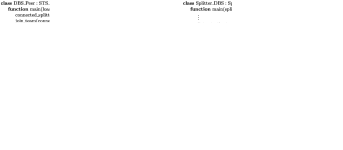
\includegraphics[width=\textwidth]{joining}
  \fig{1000}{10cm}{joining} \caption{Code related to team
    joining.\label{fig:joining}}
\end{figure*}

The new pseudo-code related to joining a team is describen in the
Fig.~\ref{fig:joining}.
\end{comment}

\begin{notex}
  See \href{https://github.com/P2PSP/simulator/blob/f0c73be1817e7d3b816cc61cd2c8e59b17f9a0e6/src/core/splitter_dbs.py#L296}{$\text{destination\_of\_chunk}[]$ in \texttt{peer\_dbs.py}}.
\end{notex}


\subsection{Buffering chunks}
%%% Local Variables:
%%% mode: latex
%%% TeX-master: "<none>"
%%% End:

\label{sec:buffering_chunks}

In order to hide the jitter generated by the physical network and the
protocol itself, peers need to store the received chunks in a buffer
during a period of time before playing them. A chunk with number $x$
is inserted in the position $(x \mathit{mod} 2B)$ of the buffer, where
$B$ is the maximum number of chunks that the buffer will store. In a
peer's life, $B$ is constant, but it is not compulsory that all peers
of the same team use the same $B$ value.

The buffer is implemented as a circular queue of $2B$ chunks, which is
filled up to only $B$ chunks in the buffering time (which is the main
part of the start-up time that the users experiment). Chunks with a
higher number (newer chunks) are inserted in the head of the
buffer. The chunk pointed by the tail of the buffer is sent to the
player (if there is a chunk in that cell of the buffer). This action
is carried out each time a new chunk is received.

Chunks can be lost.\footnote{Chunks are transmitted using a
  unrealiable communication, and therefore, network congestion can
  lose chunks.} A chunk is considered as lost when it is time to send
it to the player and the chunk has not been received.  In this
situation, for each lost chunk, the peer sends a $[\mathtt{request}
  \text{lost\_chunk\_number}]$ (that is the number of the next chunk
to be played) to the last neighbor served. When a peer $P_x$ receives
a $[\mathtt{request} \text{lost\_chunk\_number}]$ from $P_y$, $P_x$
adds $P_y$ to $\text{forward}[P_o]$, where $P_o$ is the origin peer of
the chunk stored in the position $lost\_chunk\_number$ of the buffer.

% As an alternative ...
\begin{comment}
origin peer of the next chunk stored in the
buffer. This peer has to characteristics: (1) it is not necessary a
neighbor peer, and (2) there is a high probability that this chunk has
been stored in the buffer ``for a long time'', so, if it is not a
neighbor, the link between it and the peer is working fairly well.
\end{comment}

\begin{notex}
  In the current implementation, the destination of the
  $[\mathtt{request} ...]$ message is the neighbor with the smaller
  chunk debt. This, a priori, has the drawback that this peer will
  always selected for relaying all the lost chunks because i will have
  a smaller debt as a consequence of the requests.
\end{notex}
  
In this situation, it is also possible that some peers can request
redundant paths between an origin peer and itself, and therefore, some
chunks could be received more than once. If this case, for each
duplicate chunk, a peer $P_i$ should send a $[\mathtt{prune}
  \text{duplicate\_chunk\_number}]$ message to those neighbors that
have sent to it the duplicate chunk. Neighbors receiving such message
from peer $P_i$ should remove the $P_i$ from $\text{forward}[P_o]$,
where $P_o$ is the origin peer of the duplicate chunk.

\begin{comment}
\begin{figure*}
  \fig{500}{5cm}{DBS_peer_buffering} \caption{Buffering of the
    chunks.\label{fig:DBS_peer_buffering}}
\end{figure*}
\end{comment}

The buffering time determines how much time the peers must wait before
start playing the chunks. Considering that chunks can be lost in
transit or delayed more than $B$ times of chunk, randomly, it is
difficult to determine, a priori the optimal buffering time. In the
current implementation, peers buffer a variable number of chunks that
depends on the order in which chunks are received. If $x_1$ is the
(number of the) first chunk received (the first chunk to be played),
the buffering time finishes when the chunk $x_1+B$ is
received.\footnote{Notice that all chunks with a number smaller than
  $x_1$ will be discarded, and that during the buffering time, it can
  happens that some chunks are not received on time. Therefore, it
  does not make sense to wait for $B$ chunks before stopping the
  buffering process.}

% Hablar de la relación entre B y el tamaño del team. Tal vez, cuando
% se presente la expresión de la latencia en función del grado de
% conectividad. En el caso extremo en que todos los peers se
% conectaran con todos, B >= N^*, el número máximo de peer en el team.

\begin{comment}
An heuristic that
works is the described in the Fig.~\ref{fig:DBS_peer_buffering}. As
can be seen, $\text{chunk\_to\_play}$ points to the first received
chunk, that not necessary is the received chunk with lower
index. After that, the
buffering finishes when a chunk with index $\text{chunk\_to\_play} +
\text{BUFFER\_SIZE}/2$ has been received.\footnote{This not means that
  $\text{BUFFER\_SIZE}/2$ chunks are available in the buffer.}
\end{comment}


\subsection{Chunk flooding}
\label{sec:chunk_flooding}
\begin{figure*}
  %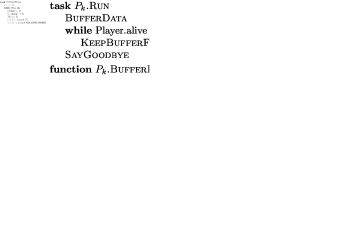
\includegraphics[width=0.75\textwidth]{chunk_generation_and_flooding}
  \fig{100}{3cm}{peer_chunk_flooding}
  \caption{Chunk flooding at peers.\label{fig:peer_chunk_flooding}}
\end{figure*}
When a peer $P_k$ receives a chunk from $P_i$, $P_k$ floods the
chunk to $T^k \setminus P_i$, using a prioritized round-robin
schema (see Fig.~\ref{fig:chunk_flooding}). Besides, if
it is a duplicate chunk, $P_k$ sends to $P_i$ a
$[\mathtt{NRFCF}~P_l]$ ($\mathtt{N}$ot $\mathtt{R}$elay
$\mathtt{F}$uture $\mathtt{C}$hunks $\mathtt{F}$rom) message, where
$P_l$ is the origin peer of the duplicate chunk. Thus, only
the first neighbor $P_i$ to send to $P_k$ a chunk
``originated'' at $P_l$ will do that in the future, at least
that $P_k$ revokes this routing information by sending a
$[\mathtt{RFCF}~P_l]$ ($\mathtt{R}$elay $\mathtt{F}$uture
$\mathtt{C}$hunks $\mathtt{F}$rom) to one or more (possibly the rest
of) peers of $T^k$.

As it has been said before, peers prioritize the flooding of the
chunks they relay by sending first the chunks to those neighbors that
are more supportive. To achieve that, every time $Pj_k$ sends a chunk
to $P_l$, $P_k$ runs $\mathtt{debt}[P_l] = \mathtt{debt}[P_l]+1$, and
$P_l$ runs $\mathtt{debt}[P_k] = \mathtt{debt}[P_k]-1$ (see
Fig.\ref{fig:}). Basically, these tables maintain a ``debt'' of chunks
between evey pair of neighbor peers. In ideal circunstances, debs
should be $0$. Debs are clipped to
$\pm\mathtt{debt}_{\text{max}}$. Obviously, a high supportivity means
a low debt, and viceversa.

\begin{comment}
In each round, peers check if a chunk have been received from the rest
of peers of the team (${\cal P}_k\in {\cal T}_j)$). If not, peers send
a $[\mathtt{propagate}~{\cal P}_i]$ to one or more (possibly
to the rest of) peers of the team, where ${\cal P}_i$ is the origin peer
of the missing chunk. At this point, the process continues as
described in Section~\ref{dbs:chunk_flooding}.
\end{comment}

\begin{comment}
For each ${\cal P}_k\in N({\cal P}_i)$, ${\cal P}_i$ checks if a chunk
has been received from ${\cal P}_k$. If ${\cal P}_i$ detects that
${\cal P}_k$ has not sent a chunk to it during $L$ consecutive rounds,
performs $N({\cal P}_i) = N({\cal P}_i)\setminus{\cal P}_k$, and stops
sending to ${\cal P}_k$ more chunks.
\end{comment}
\begin{comment}
computes a
``chunk-debt'', denoted by $d({\cal P}_k)$, that is incremented each
time a chunk is received from ${\cal P}_k$ and decremented each time a
chunk is sent to ${\cal P}_k$. If ${\cal P}_i$ verifies that $d({\cal
  P}_k)>D$ (the maximum debt), then ${\cal P}_i$ considers that ${\cal
  P}_k$ is unable to communicate with it, performs $N({\cal P}_i) =
N({\cal P}_i)\setminus{\cal P}_k$, and stops sending to ${\cal P}_k$
more chunks.
\end{comment}


%When peers receive chunks from their splitter, they must flood them to
%their neighbors until the chunks are broadcasted to the whole team
%(Fig.~\ref{fig:chunk_generation_and_flooding}). Lets suppose that
%${\cal P}_k$ receives a chunk. In the case the sender is its splitter,
%${\cal P}_k$ floods the chunk to $N({\cal P}_k)$. However, if the
%sender is a peer ${\cal P}_m\in N({\cal P}_k)$, ${\cal P}_k$ adds
%${\cal P}_m$ to $N({\cal P}_k)$ if ${\cal P}_m$ is a new neighbor, and
%forwards the chunk to the rest of its neighborhood ${\cal P}_n\in
%N({\cal P}_k)\setminus{\cal P}_m$ if ${\cal P}_k$ is in the shortest
%between ${\cal P}_n$ and the origin peer ${\cal P}_i$ of the relayed
%chunk. This will be true if ${\cal P}_k$ is the gateway of ${\cal
%  P}_n$ to go from ${\cal P}_n$ to ${\cal P}_i$. Therefore, a flooding
%with prunning based on shortest path routing is used.


\subsection{Routes discovery and topology optimization}
% Emacs, this is -*-latex-*-

% Routes Discovery and Topology Optimization

\label{sec:routes_discovery}

Chunks can be lost under bandwidth and buffering time constraints. A
chunk is lost when it is time to send it to the player, i.e. when it
is pointed by $p_p$, and the chunk has not been received. 
When a peer realizes that a chunk pointed by $p_p$ has been lost,
nothing can be done to recover it. Peers pre-fetch ``potentially
lost'' chunks at the buffer position $p_p+p_h$, where $p_h\geq 0$ is
the pre-feching horizon. Setting $p_h=0$, the pre-fetching is
disabled and only those chunks that really are lost will be
requested \leorem{no entiendo para que se piden}. 
On the contrary, the higher the $p_h$, the more aggressive
the pre-fetching is.  

For each (potentially) lost chunk with number
$\text{lost\_chunk\_number}$, peers send a
$[\mathtt{request}~\text{lost\_chunk\_number}]$ message to a random
peer of the team\leorem{solo uno? cuando se produce pruning?}. When a peer $P_i$ receives such message from 
$P_j$, $P_i$ adds $P_j$ to $\mathtt{forward}[P_k]$. $P_k$ is the
origin peer of the chunk stored in the position
$(\text{lost\_chunk\_number}~\mathit{mod}~2B)$ of $P_i$'s buffer in case this
chunks has been received. Otherwise, the request is ignored \leorem{y cómo se recupera?}. Notice
that, although request messages are very short, they are an overhead.

When request messages are used, redundant routes can be created and
therefore, some chunks could be received more than once. This is an overhead to be minimized. \leo{Upon the reception of the lost chunk, a peer send a pruning message to the other requested peers}. The receiver of the pruning message counts the number of times that a origin peer has been pruned, and when this counter is higher than a threshold $T$ (the maximum number of generated duplicates \leo{at requester's side}), the corresponding entry in the $\text{forward}[]$ table is deleted \leorem{Es por chunk o por origen?}.

Now, we can define more accurately the \gls{neighborhood-degree} (see
Sec.~\ref{sec:chunk_flooding}) as the number of different destination
peers for each possible origin that a peer forwards. For example, if a
peer $P_i$ forwards chunks from the origin $P_i$ to 10 neighbors, the
neighborhood degree of $P_i$ for the origin $P_i$ is 10, and if the
peer $P_i$ also forwards chunks from an origin $P_j$ to 5 neighbors,
the neighborhood degree of $P_i$ for the origin $P_j$ is 5\leorem{yo definiría dos tipos de grado de vecindad, el mio y el de reenvio}.

Considering the rules described before, the neighborhood degrees of
peers can decrease or increase to optimize the topology of the
overlay, by minimizing $\Delta t_b$. An increment in the degree for the origin of a requested
chunk $\text{lost\_chunk\_number}$ in $P_i$ is produced when $P_i$
recives a $[\mathtt{request}~\text{lost\_chunk\_number}]$ from a peer
that is not a neighbor, yet. On the contrary, a decrement in the
degree for the origin of a pruned chunk
$\text{duplicate\_chunk\_index}$ in $P_i$ is produced when $P_i$
receives a $[\mathtt{prune}~\text{duplicate\_chunk\_index}]$ from a
neighbor peer, for that origin. In fact, the continued use of the
requesting and pruning messages produce in a peer $P_i$ that the list
$\text{forward}[P_i]$ gets shorter (smaller \gls{neighborhood-degree})
and new entries in the table $\text{forward}[]$ are created.


%\subsection{Overlay topology optimization and the neighborhood degree}
%The neighborhood degree can also grow. When a chunk is lost, the peer
requests to receive the rest of chunks from the corresponding origin
peer to a random peer of the team. If duplicates are generated, prune
messages will remove the slower routes from that origin peer,
generating that the most reliable (and possiblely faster) route to
endure. When this happens, the requesting peer will be added to
$\mathtt{forward}[]$ (and therefore, sooner or later to
$\mathtt{pending}[]$) table of the requested peer, increasing its
neighborhood degree.


\subsection{Leaving a team}
\begin{figure*}
  %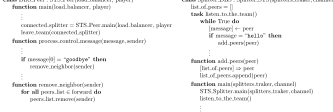
\includegraphics[width=0.55\textwidth]{leaving}
  \fig{300}{4cm}{leaving}
  \caption{Peer leaving.\label{fig:leaving}}
\end{figure*}
An outgoing peer $P^t_o$ (see Fig.~\ref{fig:leaving}) must to: (1) say
$[\mathtt{goodbye}]$ to $S^t$ and to $T^t_o$ (in this order), (2)
relay any pending (received but yet not sent) chunks, and (3) wait for
a $[\mathtt{goodbye}]$ from $S^t$, which performs $T^t = T^t \setminus
P^t_o$. In case of a timeout, $P^t_o$ resets the leaving procedure,
for a maximum number of times.

When a $P^t_k$ receives a $[\mathtt{goodbye}]$ from $P^t_o$, $P^t_k$
removes $P^t_o$ from its neighbors set, by running $T^t_k = T^t_k
\setminus P^t_o$.


\subsection{Free-riding control}
% Emacs, this is -*-latex-*-

% Free-riding Control at the Splitter

\label{sec:free_riding_control}

The splitter remembers which chunk, of a list of the last $B'$
transmitted chunks, was sent to each peer of the team. Notice that, in
order to remember the chunk that was sent to each peer in each round,
it must be hold that $B'\ge N$. \note{See
  \href{https://github.com/P2PSP/simulator/blob/f0c73be1817e7d3b816cc61cd2c8e59b17f9a0e6/src/core/splitter_dbs.py\#L296}{$\text{destination\_of\_chunk}[]$
    in \texttt{splitter\_dbs.py}}.}

Monitor peers (which are trusted peers) complain to their splitter
with a $[\mathtt{lost}~\text{lost\_chunk\_number}]$ for each lost
chunk. The splitter only considers these type of messages if they come
from a monitor.

%Notice that $L$ will
%tend to be proportional to the number $M$ of monitors, especially if
%those cases where $P_o$ is a gone peer that was unable to transmit the
%$[\mathtt{goodbye}]$ messages.

\begin{notex}
This last functionality has not been implemented, at least, as it has
been explained here. The forget() thread is controlled by a timer, not
by a counter of rounds.
\end{notex}

%Peers also control that at least one chunk is received from a neighbor
%in each round.\footnote{Peers recognize that a new round has started
%  when a new chunk is received from the splitter.} If happens that a
%peer $P_x$ does not receives a chunk from peer $P_y$ between $D^*$
%consecutive rounds, $P_x$ removes $P_y$ of its forwaring table.


%\subsection{Free-riding control at peers} % Neighborhood dynamics
%\label{dbs:frcp}
%Every time ${\cal P}^j_k$ sends a chunk to ${\cal P}^j_l$, ${\cal
P}^j_k$ runs $\mathtt{debt}[{\cal P}^j_l] = \mathtt{debt}[{\cal
P}^j_l]+1$, and ${\cal P}^j_l$ runs $\mathtt{debt}[{\cal P}^j_k]
= \mathtt{debt}[{\cal P}^j_k]-1$ (see Fig.\ref{fig}). Basically, these tables
maintain a ``debt'' of chunks between evey pair of neighbor
peers. If ${\cal P}^j_k$ realises that $\mathtt{debt}[{\cal
P}^j_l]>\mathtt{debt}_\text{max}$, then ${\cal P}^j_k$ removes ${\cal
P}^j_l$ from ${\cal T}^j_k$. Debts are clipped to $0$.

\begin{comment}
In each round, peers check if a chunk have been received from the rest
of peers of the team (${\cal P}_k\in {\cal T}_j)$). If not, peers send
a $[\mathtt{propagate}~{\cal P}_i]$ to one or more (possibly
to the rest of) peers of the team, where ${\cal P}_i$ is the origin peer
of the missing chunk. At this point, the process continues as
described in Section~\ref{dbs:chunk_flooding}.
\end{comment}

\begin{comment}
For each ${\cal P}_k\in N({\cal P}_i)$, ${\cal P}_i$ checks if a chunk
has been received from ${\cal P}_k$. If ${\cal P}_i$ detects that
${\cal P}_k$ has not sent a chunk to it during $L$ consecutive rounds,
performs $N({\cal P}_i) = N({\cal P}_i)\setminus{\cal P}_k$, and stops
sending to ${\cal P}_k$ more chunks.
\end{comment}
\begin{comment}
computes a
``chunk-debt'', denoted by $d({\cal P}_k)$, that is incremented each
time a chunk is received from ${\cal P}_k$ and decremented each time a
chunk is sent to ${\cal P}_k$. If ${\cal P}_i$ verifies that $d({\cal
  P}_k)>D$ (the maximum debt), then ${\cal P}_i$ considers that ${\cal
  P}_k$ is unable to communicate with it, performs $N({\cal P}_i) =
N({\cal P}_i)\setminus{\cal P}_k$, and stops sending to ${\cal P}_k$
more chunks.
\end{comment}


%\subsection{Congestion control}
%\label{dbs:congestion_control}
%P2PSP is a content-unaware push-based protocol. To avoid network
congestion while flooding, sending peers must perform some kind of
data flow-control. Moreover, to achieve aN ideal I/O ratio of $1$,
peers should send one chunk for every received one.

Congestion control in P2PSP is very simple: if a new chunk is
received, peers forward (using the flooding with prunning algorithm
described in Sec~\ref{dbs:chunk_generation_and_flooding}) each
received chunk to the next peer of their list of peers (following a
round-robin pattern).

%Peers do not understand the content, but it is
%known that in order to achieve a I/O ratio of 1, peers should send one
%chunk for every received one, on average. To acomplish this, a ${\cal
%  P}_i$ creates a FIFO queue of chunks for each $N({\cal P}_i)$, and,
%for each received chunk, ${\cal P}_i$ forwards a queued chunk from
%each of these queues.

\begin{comment}
A ${\cal P}_i$ forwards one or more chunks if and only if it has
received a chunk. For each received chunk $c_j$, ${\cal P}_i$: 1)
creates a list $l_{c_j}$ with the contents of $N'({\cal P}_i)$, and 2)
sends $c_j$ to $l_{c_j}[0]$ (the first element), and removes
$l_{c_j}[0]$. For each chunk reception, Step 2) is repeated for all
the previously created lists while they are not exhausted.

A solution is a forwarding algorithm based on the following
idea. Peers manage a list of chunks, where every item is a 2-tuple
($c_k$, $P_l$). The field $c_k$ represents the chunk that must be
flooded (if the node that has delivered the chunk is the splitter,
$c_k$ must be relayed towards all the neighbors, otherwise, $c_k$ must
be sent to all the neighbors except the peer that delivered $c_k$),
and the field $P_l$ the last neighbor to which $c_k$ was sent. For
every chunk received, a new tuple is appended to the list of chunks
and the rest of tuples are updated. The field $c_k$ remains constant
but $P_l$ is replaced by the next peer in the list of neighbors for
every received chunk.
\end{comment}


\begin{comment}
\subsubsection{Flooding order}
\label{dbs:flooding_order}
As an incentive mechanism~\cite{xu2006analysis}, peers relay received
chunks first to those peers that 
\end{comment}

%neighbors with lower chunk-debts.

\begin{comment}
\subsubsection{Team dynamics}
\label{dbs:team_dynamics}
${\cal P}_i$ adds to $N({\cal P}_i)$ those ${\cal P}_j$ that has sent
to ${\cal P}_i$ a chunk. If $N({\cal P}_i)>K$, periodically, ${\cal
  P}_i$ removes from $N({\cal P}_i)$ the peer with highest chunk-debt
and try to find in ${\cal T}_j\setminus N({\cal P}_i)$ a new peer using
$[\mathtt{hello}]$ messages.
\end{comment}

\begin{comment}
Peers use a buffer $b$ of chunks to hide the jitter generated by the
physical network and the broadcasting protocol. When a peer receives
$C_i$, it performs
\begin{equation}
  b[i~\text{mod}~B] = c_i,
\end{equation}
where ``mod'' represents the modulo operator and $B$ the buffer size
(in chunks). Basically, the buffer represents a sliding window that
moves over the stream synchronizely with the playing because the the
player consumes the chunks at the same chunk-rate the source produces
them.
\end{comment}

%%%%%%%%%%

\begin{comment}

\begin{itemize}

\item In the P2PSP, only monitor peers complains about lost
  chunks. This means that if a chunk that has been retransmitted by a
  peer is lost, it will be only retransmitted to all the peers of the
  team if the destination is a monitor peer and there is a unique
  monitor peer in the team. On the other hand, if the lost chunk was
  traveling from the splitter to a peer, all monitor peers will
  complain and this chunk will be retransmitted to the complete
  team. Therefore, only massively loss chunks will be retransmitted in
  the P2PSP. However, notice that a isolated missing chunk will
  produce negligible artifacts in the playback of one peer. In the
  Chain model, the lost of a chunk is handled between neighbour peers
  which means that all lost blocks should be, a priori, recovered.

\end{itemize}

\end{comment}



\begin{comment}
\subsubsection{Shortest path computation}
\label{dbs:chunk_routing}
\begin{figure}
  %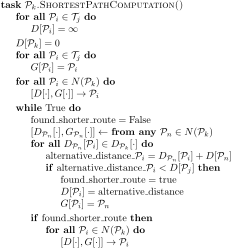
\includegraphics[width=0.35\textwidth]{shortest_path_computation}
  \fig{500}{4cm}{shortest_path_computation}
  \caption{Shortest path computation.\label{fig:shortest_path_computation}}
\end{figure}
The shortest path distances among peers are determined by a variation
of the Bellman-Ford Algorithm~\cite{Bertsekas1987data} (see
Fig.~\ref{fig:shortest_path_computation}), where the cost of the
``links'' between neighbor peers is $1$. Neighbor peers interchange
two vectors $D[\cdot]$ (distance-to-peer) and $G[\cdot]$
(gateway-to-peer) and compute the shortest distances and the (peer)
gateways to (reach) the rest of peers of its team ${\cal T}_j$.

This algorithm is free of routing loops and is not suceptible of the
well known count-to-infinity problem, and therefore always converges
for static teams. These problems do not appear because the routes are 

Each peer ${\cal P}_k$ sends
its vector of distances $D[\forall {\cal P}_i\in T^*({\cal P}_k)]$ and
gateways $G[\forall {\cal P}_i\in T^*({\cal P}_k)]$ to each
neighbor. When this information is received, peers check if shorter
routes can be found to the rest of peers of the reachable team, and if
so, send these vectors again.

The Bellman-Ford algorithm is susceptible of routing loops and the
count-to-infinite problem.


% Hace falta saber desde dónde viene el chunk original (origin peer) y que todos los peers dispongan de los vector-distances de los peers vecinos. Los vector-ditances deben tener tantas entradas como peers existen en el team. Por tanto, cada peer almacena un número de vector-distances igual a su grado de conectividad.


% Supposing that the weight of links between neighbors is 1.
% ¿Cómo sabe un peer que él es el último?
\end{comment}

\begin{comment}
\subsubsection{Generation of the routing tables}
Routing tables has as many entries as peers are in the team. The
routing table of a peer $P_i$ is a dictionary of pairs ($d(P_i, P_j)$,
$P_k$) indexed by the destination peer $P_j$ is a destination peer,
where $d(P_i, P_j)$ is the last measurement of the number of hops (in
peers) between $P_i$ and $P_j$, and $P_k\in N(P_i)$ is the 1-hop peer
that in the shortest-path between $P_i$ and $P_j$. Notice that if
$P_j==P_k$ then $d(P_i, P_j)==1$, which means that $P_i$ and $P_j$ are
directly ``connected''.

When a peer has updated its routing table, it is sent to their
neighbors pyggibacked on a \textsf{chunk} packet. When a peer receives
a routing table, it keeps a copy of it and updates its own routing
table with the new routing information using the Bellman-Ford
Algorithm~\cite{}. The peers have a copy of the routing table of its
neighbors to use it through the chunk routing process (see
Rule~\cite{the_routing_process}.
\end{comment}



\end{comment}

\bibliography{networking,P2P,streaming,misc,simulcasting,SVC,MDC,local}
